% =============================================================================
% APRESENTAÇÃO APS2 — versão 2 (estrutura de cartões, etiquetas e faixas)
% Tema UFG (capa, divisórias e encerramento) + slides de conteúdo desenhados em TikZ.
% Compilar: tectonic apresentacao-aps2-v2.tex
% =============================================================================
\documentclass[aspectratio=169,t,xcolor=table]{beamer}
\usepackage[utf8]{inputenc}
\usepackage[brazil]{babel}
\usepackage{booktabs}
\usepackage{listings}
\usepackage{graphicx}
\usepackage{tikz}
\usetikzlibrary{calc}

\usetheme{Ufg}
\graphicspath{{../assets/}{../assets/simbolos/}{figs/}}
\setbeamersize{text margin left=0.05\textwidth, text margin right=0.05\textwidth}

% ------------------------------------------------------------------ cores
\definecolor{Navy}{RGB}{0,92,161}        % INFBlue
\definecolor{Claro}{RGB}{226,238,248}
\definecolor{Fundo}{RGB}{245,247,250}
\definecolor{Borda}{RGB}{220,226,234}
\definecolor{Texto}{RGB}{33,33,33}
\definecolor{Cinza}{RGB}{100,116,139}
\definecolor{Destaque}{RGB}{255,193,7}   % LightOrange do tema
\definecolor{Principal}{RGB}{0,114,185}  % casos principais (azul)
\definecolor{Apoio}{RGB}{240,170,20}     % casos de apoio (amarelo)
\definecolor{PFront}{RGB}{0,114,185}
\definecolor{PBack}{RGB}{91,141,8}
\definecolor{PInt}{RGB}{240,170,20}
\definecolor{PExt}{RGB}{142,36,170}
\definecolor{PDados}{RGB}{214,96,96}

\newcommand{\inc}{\guillemotleft include\guillemotright}
\newcommand{\ext}{\guillemotleft extend\guillemotright}

% ------------------------------------------------------------------ layout base
\newcommand{\setLayoutClean}{\usebackgroundtemplate{}\setDefaultConfig}

\newcommand{\slideDiagrama}[2]{%
    \begin{frame}[plain]
        \vspace{0.12cm}\centering
        {\normalsize\sffamily\bfseries\color{UFGBlue} #1}\par\vspace{0.08cm}\vfill
        \makebox[\textwidth][c]{\includegraphics[width=0.96\paperwidth,height=0.86\paperheight,keepaspectratio]{#2}}%
        \vfill
    \end{frame}}
\newcommand{\slideRegiao}[3]{%
    \begin{frame}[plain]
        \vspace{0.12cm}\centering
        {\normalsize\sffamily\bfseries\color{UFGBlue} #1}\par\vspace{0.08cm}\vfill
        \makebox[\textwidth][c]{\includegraphics[trim=#3,clip,width=0.96\paperwidth,height=0.86\paperheight,keepaspectratio]{#2}}%
        \vfill
    \end{frame}}

\AtBeginSection[]{%
    \setLayout{mainpoint}\setBGColor{UFGBlue}%
    \begin{frame}[plain,noframenumbering]{}\frametitle{\fonteTela\LARGE\insertsectionnumber.\ \insertsectionhead}\end{frame}%
    \setLayoutClean}

% ponto em pt a partir do canto superior esquerdo da página (160 x 90 mm)
\newcommand{\pto}[2]{($(current page.north west)+({(#1)*1pt},{-(#2)*1pt})$)}

% fundo: etiqueta-escura etiqueta-clara título subtítulo
\newcommand{\fundo}[4]{%
  \fill[Fundo] (current page.south west) rectangle (current page.north east);
  \shade[left color=Navy, right color=UFGBlue]
    (current page.south west) rectangle ($(current page.south east)+(0,14pt)$);
  \node[anchor=north west, inner xsep=5pt, inner ysep=2.3pt, fill=Navy, rounded corners=6pt, text=white,
        font=\sffamily\fontsize{5.5pt}{6.4pt}\selectfont\bfseries] (pa) at \pto{25}{12} {#1};
  \node[anchor=west, inner xsep=5pt, inner ysep=2.3pt, fill=Claro, rounded corners=6pt, text=Navy,
        font=\sffamily\fontsize{5.5pt}{6.4pt}\selectfont\bfseries] at ($(pa.east)+(4pt,0)$) {#2};
  \node[anchor=north west, inner sep=0pt, text=Navy, text width=380pt, align=flush left] at \pto{25}{27}
    {\fontsize{15pt}{17pt}\selectfont\bfseries #3\par};
  \node[anchor=north west, inner sep=0pt, text=Cinza, text width=404pt, align=flush left] at \pto{25}{50}
    {\fontsize{7.3pt}{9.2pt}\selectfont #4\par};
  \node[anchor=north east, inner sep=0pt] at \pto{429}{12}
    {
\includegraphics[height=20pt]{lib/logos/INF-compact-black.png}};
  \node[anchor=south west, inner sep=0pt, text=white] at \pto{25}{251}
    {\fontsize{4.8pt}{5.5pt}\selectfont Modelagem de Software · APS2 · Site de Loja de Eletrônicos · UFG/INF};
  \node[anchor=south east, inner sep=0pt, text=white] at \pto{429}{251}
    {\fontsize{5pt}{5.5pt}\selectfont Grupo 4 \quad|\quad \insertframenumber\ / \inserttotalframenumber};
}

% marca de destaque (canto dos quadros)
\newcommand{\gota}[2]{\fill[Destaque] \pto{#1}{#2} circle (3.2pt); \fill[Destaque] \pto{#1}{#2} rectangle ++(3.2pt,3.2pt);}

% cartão com barra lateral: x y larg alt cor título texto
\newcommand{\cartao}[7]{%
  \fill[white] \pto{#1}{#2} rectangle \pto{#1+#3}{#2+#4};
  \draw[Borda, line width=0.5pt] \pto{#1}{#2} rectangle \pto{#1+#3}{#2+#4};
  \fill[#5] \pto{#1}{#2} rectangle \pto{#1+3}{#2+#4};
  \node[anchor=north west, inner sep=0pt, text=Navy, text width={(#3-18)*1pt}, align=flush left] at \pto{#1+11}{#2+6}
    {\fontsize{8.4pt}{10pt}\selectfont\bfseries #6\par\vspace{2pt}
     {\color{Texto}\fontsize{6.6pt}{8.3pt}\selectfont\mdseries #7\par}};
}

% faixa larga: y alt cor título texto
\newcommand{\faixa}[5]{%
  \fill[white] \pto{25}{#1} rectangle \pto{429}{#1+#2};
  \draw[Borda, line width=0.5pt] \pto{25}{#1} rectangle \pto{429}{#1+#2};
  \fill[#3] \pto{25}{#1} rectangle \pto{28}{#1+#2};
  \node[anchor=west, inner sep=0pt, text=Navy, text width=104pt, align=flush left] at \pto{38}{#1+#2/2}
    {\fontsize{7.8pt}{9.2pt}\selectfont\bfseries #4\par};
  \node[anchor=west, inner sep=0pt, text=Texto, text width=274pt, align=flush left] at \pto{146}{#1+#2/2}
    {\fontsize{6.7pt}{8.4pt}\selectfont #5\par};
}

% quadro de número (claro e escuro): x y larg alt número rótulo detalhe
\newcommand{\tile}[7]{%
  \fill[white] \pto{#1}{#2} rectangle \pto{#1+#3}{#2+#4};
  \draw[Borda, line width=0.5pt] \pto{#1}{#2} rectangle \pto{#1+#3}{#2+#4};
  \gota{#1+#3-11}{#2+11}
  \node[anchor=north west, inner sep=0pt, text=Navy] at \pto{#1+11}{#2+7} {\fontsize{24pt}{26pt}\selectfont\bfseries #5\par};
  \node[anchor=north west, inner sep=0pt, text=Navy, text width={(#3-22)*1pt}, align=flush left] at \pto{#1+11}{#2+37}
    {\fontsize{7.6pt}{9.2pt}\selectfont\bfseries #6\par\vspace{1.5pt}{\color{Cinza}\fontsize{6.4pt}{8pt}\selectfont\mdseries #7\par}};
}
\newcommand{\tileD}[7]{%
  \fill[Navy] \pto{#1}{#2} rectangle \pto{#1+#3}{#2+#4};
  \gota{#1+#3-11}{#2+11}
  \node[anchor=north west, inner sep=0pt, text=white] at \pto{#1+11}{#2+7} {\fontsize{24pt}{26pt}\selectfont\bfseries #5\par};
  \node[anchor=north west, inner sep=0pt, text=white, text width={(#3-22)*1pt}, align=flush left] at \pto{#1+11}{#2+37}
    {\fontsize{7.6pt}{9.2pt}\selectfont\bfseries #6\par\vspace{1.5pt}{\color{white!85!Navy}\fontsize{6.4pt}{8pt}\selectfont\mdseries #7\par}};
}

% cartão de decisão numerado: x y larg alt número título etiqueta texto
\newcommand{\decisao}[8]{%
  \fill[white] \pto{#1}{#2} rectangle \pto{#1+#3}{#2+#4};
  \draw[Borda, line width=0.5pt] \pto{#1}{#2} rectangle \pto{#1+#3}{#2+#4};
  \fill[Destaque] \pto{#1+15}{#2+15} circle (7.5pt);
  \node[text=Navy, inner sep=0pt] at \pto{#1+15}{#2+15} {\fontsize{8pt}{9pt}\selectfont\bfseries #5\par};
  \node[anchor=west, inner sep=0pt, text=Navy, text width={(#3-36)*1pt}, align=flush left] at \pto{#1+28}{#2+15}
    {\fontsize{7.8pt}{9pt}\selectfont\bfseries #6\par};
  \node[anchor=north west, inner xsep=3.5pt, inner ysep=1.6pt, draw=UFGBlue, fill=white, rounded corners=3pt,
        text=UFGBlue, line width=0.6pt, font=\sffamily\fontsize{5.2pt}{6pt}\selectfont\bfseries] at \pto{#1+10}{#2+29} {#7};
  \node[anchor=north west, inner sep=0pt, text=Texto, text width={(#3-20)*1pt}, align=flush left] at \pto{#1+10}{#2+43}
    {\fontsize{6.5pt}{8.2pt}\selectfont #8\par};
}

% linha compacta: y alt cor nome texto rótulo cor-do-texto-do-rótulo
\newcommand{\linha}[7]{%
  \fill[white] \pto{25}{#1} rectangle \pto{429}{#1+#2};
  \draw[Borda, line width=0.5pt] \pto{25}{#1} rectangle \pto{429}{#1+#2};
  \fill[#3] \pto{25}{#1} rectangle \pto{28}{#1+#2};
  \node[anchor=west, inner sep=0pt, text=Navy, text width=120pt, align=flush left] at \pto{36}{#1+#2/2}
    {\fontsize{7pt}{8.2pt}\selectfont\bfseries #4\par};
  \node[anchor=west, inner sep=0pt, text=Texto, text width=196pt, align=flush left] at \pto{160}{#1+#2/2}
    {\fontsize{6.6pt}{8pt}\selectfont #5\par};
  \node[anchor=east, inner xsep=4pt, inner ysep=1.6pt, fill=#3, rounded corners=3pt, text=#7,
        font=\sffamily\fontsize{5.3pt}{6.2pt}\selectfont\bfseries] at \pto{421}{#1+#2/2} {#6};
}

% linha com símbolo: y alt imagem nome texto
\newcommand{\linhasimb}[5]{%
  \fill[white] \pto{25}{#1} rectangle \pto{429}{#1+#2};
  \draw[Borda, line width=0.5pt] \pto{25}{#1} rectangle \pto{429}{#1+#2};
  \fill[Navy] \pto{25}{#1} rectangle \pto{28}{#1+#2};
  \node[inner sep=0pt] at \pto{80}{#1+#2/2} {\includegraphics[height=\dimexpr #2pt-8pt\relax,width=92pt,keepaspectratio]{#3}};
  \node[anchor=west, inner sep=0pt, text=Navy, text width=96pt, align=flush left] at \pto{140}{#1+#2/2}
    {\fontsize{7.4pt}{8.6pt}\selectfont\bfseries #4\par};
  \node[anchor=west, inner sep=0pt, text=Texto, text width=180pt, align=flush left] at \pto{244}{#1+#2/2}
    {\fontsize{6.7pt}{8.2pt}\selectfont #5\par};
}

% passo numerado: x y larg alt número texto [etiqueta] [cor-etiqueta] [cor-texto-etiqueta]
\newcommand{\passo}[9]{%
  \fill[white] \pto{#1}{#2} rectangle \pto{#1+#3}{#2+#4};
  \draw[Borda, line width=0.5pt] \pto{#1}{#2} rectangle \pto{#1+#3}{#2+#4};
  \fill[Destaque] \pto{#1+14}{#2+#4/2} circle (6.2pt);
  \node[text=Navy, inner sep=0pt] at \pto{#1+14}{#2+#4/2} {\fontsize{6.8pt}{8pt}\selectfont\bfseries #5\par};
  \node[anchor=west, inner sep=0pt, text=Texto, text width={(#3-92)*1pt}, align=flush left] at \pto{#1+26}{#2+#4/2}
    {\fontsize{6.8pt}{8.2pt}\selectfont #6\par};
  \node[anchor=east, inner xsep=4pt, inner ysep=1.6pt, fill=#8, rounded corners=3pt, text=#9,
        font=\sffamily\fontsize{5.2pt}{6pt}\selectfont\bfseries] at \pto{#1+#3-7}{#2+#4/2} {#7};
}

% seta encadeada (chevron): x y larg alt cor-fundo cor-texto título texto
\newcommand{\chev}[8]{%
  \fill[#5] \pto{#1}{#2} -- \pto{#1+#3-10}{#2} -- \pto{#1+#3}{#2+#4/2} -- \pto{#1+#3-10}{#2+#4}
            -- \pto{#1}{#2+#4} -- \pto{#1+10}{#2+#4/2} -- cycle;
  \node[anchor=west, inner sep=0pt, text=#6, text width={(#3-30)*1pt}, align=flush left] at \pto{#1+17}{#2+#4/2}
    {\fontsize{7pt}{8.4pt}\selectfont\bfseries #7\par\vspace{1pt}{\fontsize{5.8pt}{7pt}\selectfont\mdseries #8\par}};
}

% cartão de relacionamento com símbolo: x y larg alt cor título texto imagem
\newcommand{\tipo}[8]{%
  \fill[white] \pto{#1}{#2} rectangle \pto{#1+#3}{#2+#4};
  \draw[Borda, line width=0.5pt] \pto{#1}{#2} rectangle \pto{#1+#3}{#2+#4};
  \fill[#5] \pto{#1}{#2} rectangle \pto{#1+3}{#2+#4};
  \node[anchor=north west, inner sep=0pt, text=Navy, text width={(#3-110)*1pt}, align=flush left] at \pto{#1+11}{#2+7}
    {\fontsize{8.4pt}{10pt}\selectfont\bfseries #6\par\vspace{2pt}{\color{Texto}\fontsize{6.5pt}{8.2pt}\selectfont\mdseries #7\par}};
  \node[inner sep=0pt] at \pto{#1+#3-50}{#2+#4/2} {\includegraphics[width=84pt,height=\dimexpr #4pt-14pt\relax,keepaspectratio]{#8}};
}

% painel escuro com mensagem principal: x y larg alt etiqueta título texto
\newcommand{\painel}[7]{%
  \fill[Navy] \pto{#1}{#2} rectangle \pto{#1+#3}{#2+#4};
  \gota{#1+#3-11}{#2+11}
  \node[anchor=north west, inner sep=0pt, text=Destaque] at \pto{#1+13}{#2+12} {\fontsize{5.8pt}{6.6pt}\selectfont\bfseries #5\par};
  \node[anchor=north west, inner sep=0pt, text=white, text width={(#3-26)*1pt}, align=flush left] at \pto{#1+13}{#2+26}
    {\fontsize{11pt}{13.5pt}\selectfont\bfseries #6\par};
  \node[anchor=south west, inner sep=0pt, text=white, text width={(#3-26)*1pt}, align=flush left] at \pto{#1+13}{#2+#4-10}
    {\fontsize{6.7pt}{8.6pt}\selectfont #7\par};
}

% cartão de caso de uso padronizado: x y larg alt cor título cabeçalho passos alternativos
\newcommand{\cucard}[9]{%
  \fill[white] \pto{#1}{#2} rectangle \pto{#1+#3}{#2+#4};
  \draw[Borda, line width=0.5pt] \pto{#1}{#2} rectangle \pto{#1+#3}{#2+#4};
  \fill[#5] \pto{#1}{#2} rectangle \pto{#1+3}{#2+#4};
  \node[anchor=north west, inner sep=0pt, text=Navy, text width={(#3-18)*1pt}, align=flush left] at \pto{#1+11}{#2+6}
    {\fontsize{8.2pt}{9.6pt}\selectfont\bfseries #6\par\vspace{2.5pt}
     {\color{Texto}\fontsize{6.1pt}{7.45pt}\selectfont\mdseries #7\par\vspace{2.5pt}
      {\color{Navy}\bfseries Fluxo:}\par #8\par\vspace{2.5pt}
      {\color{Navy}\bfseries Alternativos:}\par #9\par}};
}
\newcommand{\cucardL}[9]{%
  \fill[white] \pto{#1}{#2} rectangle \pto{#1+#3}{#2+#4};
  \draw[Borda, line width=0.5pt] \pto{#1}{#2} rectangle \pto{#1+#3}{#2+#4};
  \fill[#5] \pto{#1}{#2} rectangle \pto{#1+3}{#2+#4};
  \node[anchor=north west, inner sep=0pt, text=Navy, text width={(#3-18)*1pt}, align=flush left] at \pto{#1+11}{#2+6}
    {\fontsize{8.8pt}{10.4pt}\selectfont\bfseries #6\par\vspace{3pt}
     {\color{Texto}\fontsize{6.6pt}{8pt}\selectfont\mdseries #7\par\vspace{3pt}
      {\color{Navy}\bfseries Fluxo:}\par #8\par\vspace{3pt}
      {\color{Navy}\bfseries Alternativos:}\par #9\par}};
}

\newfontfamily\fonteTela{Roboto}[Extension=.otf, UprightFont=*-Regular, BoldFont=*-Bold, ItalicFont=*-Italic, BoldItalicFont=*-BoldItalic, Ligatures=TeX]
\renewcommand{\sffamily}{\fonteTela}
\setmainfont{Roboto}[Extension=.otf, UprightFont=*-Regular, BoldFont=*-Bold, ItalicFont=*-Italic, BoldItalicFont=*-BoldItalic, Ligatures=TeX]
\renewcommand{\familydefault}{\rmdefault}

% ------------------------------------------------------------------ v3: diagrama + painel
% destaque sobre o diagrama: x0 y0 x1 y1 cor
\newcommand{\hl}[5]{\draw[#5, line width=1.3pt, rounded corners=3pt, fill=#5, fill opacity=0.10] \pto{#1}{#2} rectangle \pto{#3}{#4};}
% marcador numerado: x y número
\newcommand{\mk}[3]{\fill[white] \pto{#1}{#2} circle (6.6pt); \fill[Destaque] \pto{#1}{#2} circle (5.6pt);
  \node[text=Navy, inner sep=0pt] at \pto{#1}{#2} {\fontsize{6.6pt}{7pt}\selectfont\bfseries #3};}
% rótulo sobre o diagrama: x y cor-fundo cor-texto texto
\newcommand{\rot}[5]{\node[anchor=center, inner xsep=3.5pt, inner ysep=1.6pt, fill=#3, rounded corners=3pt, text=#4,
  font=\sffamily\fontsize{5.6pt}{6.4pt}\selectfont\bfseries] at \pto{#1}{#2} {#5};}
% marcador em linha de texto
\newcommand{\nmk}[1]{\tikz[baseline=(n.base)]\node[circle, fill=Destaque, text=Navy, inner sep=0.8pt, minimum size=8.5pt,
  font=\sffamily\fontsize{5.6pt}{6pt}\selectfont\bfseries](n){#1};}
% cartão do painel: x y larg alt cor título texto
\newcommand{\pcard}[7]{%
  \fill[white] \pto{#1}{#2} rectangle \pto{#1+#3}{#2+#4};
  \draw[Borda, line width=0.5pt] \pto{#1}{#2} rectangle \pto{#1+#3}{#2+#4};
  \fill[#5] \pto{#1}{#2} rectangle \pto{#1+3}{#2+#4};
  \node[anchor=north west, inner sep=0pt, text=Navy, text width={(#3-15)*1pt}, align=flush left] at \pto{#1+9}{#2+5}
    {\fontsize{7.3pt}{8.6pt}\selectfont\bfseries #6\par\vspace{1.5pt}
     {\color{Texto}\fontsize{6.3pt}{7.6pt}\selectfont\mdseries #7\par}};
}
% linha numerada do painel: x y larg alt número texto
\newcommand{\pnum}[6]{%
  \fill[white] \pto{#1}{#2} rectangle \pto{#1+#3}{#2+#4};
  \draw[Borda, line width=0.5pt] \pto{#1}{#2} rectangle \pto{#1+#3}{#2+#4};
  \fill[Destaque] \pto{#1+10}{#2+#4/2} circle (5.4pt);
  \node[text=Navy, inner sep=0pt] at \pto{#1+10}{#2+#4/2} {\fontsize{6.3pt}{7pt}\selectfont\bfseries #5};
  \node[anchor=west, inner sep=0pt, text=Texto, text width={(#3-27)*1pt}, align=flush left] at \pto{#1+20}{#2+#4/2}
    {\fontsize{6.3pt}{7.6pt}\selectfont #6\par};
}
% caso de uso no painel: x y larg alt cor título cabeçalho passos alternativos
\newcommand{\pcu}[9]{%
  \fill[white] \pto{#1}{#2} rectangle \pto{#1+#3}{#2+#4};
  \draw[Borda, line width=0.5pt] \pto{#1}{#2} rectangle \pto{#1+#3}{#2+#4};
  \fill[#5] \pto{#1}{#2} rectangle \pto{#1+3}{#2+#4};
  \node[anchor=north west, inner sep=0pt, text=Navy, text width={(#3-15)*1pt}, align=flush left] at \pto{#1+9}{#2+5}
    {\fontsize{7.4pt}{8.6pt}\selectfont\bfseries #6\par\vspace{1.5pt}
     {\color{Texto}\fontsize{5.9pt}{6.85pt}\selectfont\mdseries #7\par\vspace{1.2pt}
      {\color{Navy}\bfseries Fluxo:}\par #8\par\vspace{1.2pt}
      {\color{Navy}\bfseries Alternativos:}\par #9\par}};
}

\newenvironment{tela}{\linespread{1}\fonteTela\selectfont\begin{tikzpicture}[remember picture, overlay]}{\end{tikzpicture}}

% ------------------------------------------------------------------ identificação
\setPrimaryColor{UFGBlue}
\setLogos{lib/logos/INF-compact-white.png}{lib/logos/INF-compact-white.png}
\title[Loja de Eletrônicos --- APS2]{Site de Loja de Eletrônicos (E-commerce)}
\subtitle{Modelagem de Software --- APS2}
\author[Grupo 4]{%
  Carlos Eduardo Freire da Silva \and Gabriel Henrique Lourenço Dias \and Kayque Vicente Silva\\
  Luiz Pedro Pereira Mendes Saraiva \and Yury Nogueira de Oliveira Silva}
\institute[UFG/INF]{%
  Instituto de Informática (INF) --- Universidade Federal de Goiás (UFG)\\
  Bacharelado em Engenharia de Software --- Prof. Me. Diogo Oliveira Santos}
\date{2026/2}

\begin{document}

\setLayout{titlepage}
\frame[noframenumbering]{\titlepage}

\setLayoutClean
\begin{frame}[plain,noframenumbering]{Sumário}
    \vspace{0.3cm}
    \tableofcontents
\end{frame}

% =============================================================================
\section{Visão Geral do Sistema}
% =============================================================================

% --- Carlos ---
\begin{frame}[plain]\begin{tela}
  \fundo{1.1 · 1.2}{VISÃO GERAL}{Uma loja virtual de eletrônicos}
    {Catálogo, carrinho e pedido para o cliente; produtos, estoque e pedidos para a loja}
  \cartao{25}{70}{128}{74}{PFront}{O Cliente}{Navega com filtros por categoria, marca e preço, monta o carrinho e finaliza o pedido.}
  \cartao{163}{70}{128}{74}{PInt}{Serviços Externos}{Gateway de pagamento e serviço de frete; avisos por e-mail.}
  \cartao{301}{70}{128}{74}{PBack}{Área Administrativa}{Produtos, estoque e status dos pedidos.}
  \faixa{152}{38}{Navy}{Dentro do escopo}{Cadastro e login, catálogo, carrinho, finalização com frete e pagamento, consulta e cancelamento de pedidos, área administrativa e avisos por e-mail.}
  \faixa{196}{34}{Destaque}{Fora do escopo}{Cupons, avaliações, troca e devolução, nota fiscal, marketplace e aplicativo nativo.}
\end{tela}\end{frame}

% --- Carlos ---
\begin{frame}[plain]\begin{tela}
  \fundo{1.3}{PREMISSAS}{Premissas que fecham as lacunas do tema}
    {Suposições do grupo, registradas no documento}
  \cartao{25}{70}{128}{78}{Navy}{Web app responsivo}{Celular e computador; sem aplicativo nativo.}
  \cartao{163}{70}{128}{78}{Navy}{Login só ao finalizar}{O visitante monta o carrinho sem conta.}
  \cartao{301}{70}{128}{78}{Navy}{Um perfil administrativo}{Um único tipo de administrador.}
  \cartao{25}{154}{128}{78}{Destaque}{Cartão, Pix ou boleto}{Sempre pelo gateway de pagamento.}
  \cartao{163}{154}{128}{78}{Destaque}{Só e-mail}{Único canal de aviso ao cliente.}
  \cartao{301}{154}{128}{78}{Destaque}{Prazo de pagamento}{Pedido não pago é cancelado após um prazo; o estoque volta.}
\end{tela}\end{frame}

% =============================================================================
\section{Diagrama de Casos de Uso}
% =============================================================================

% --- Carlos ---
\begin{frame}[plain]\begin{tela}
  \fundo{2.1}{ATORES}{Três usuários e três sistemas externos}
    {13 casos de uso: 7 principais (azul) e 6 de apoio (amarelo) --- Figura 1 e Tabela 1}
  \fill[white] \pto{25}{64} rectangle \pto{223.1889081455806}{237};
  \draw[Borda, line width=0.5pt] \pto{25}{64} rectangle \pto{223.1889081455806}{237};
  \node[anchor=north west, inner sep=0pt] at \pto{28.0}{64.0} {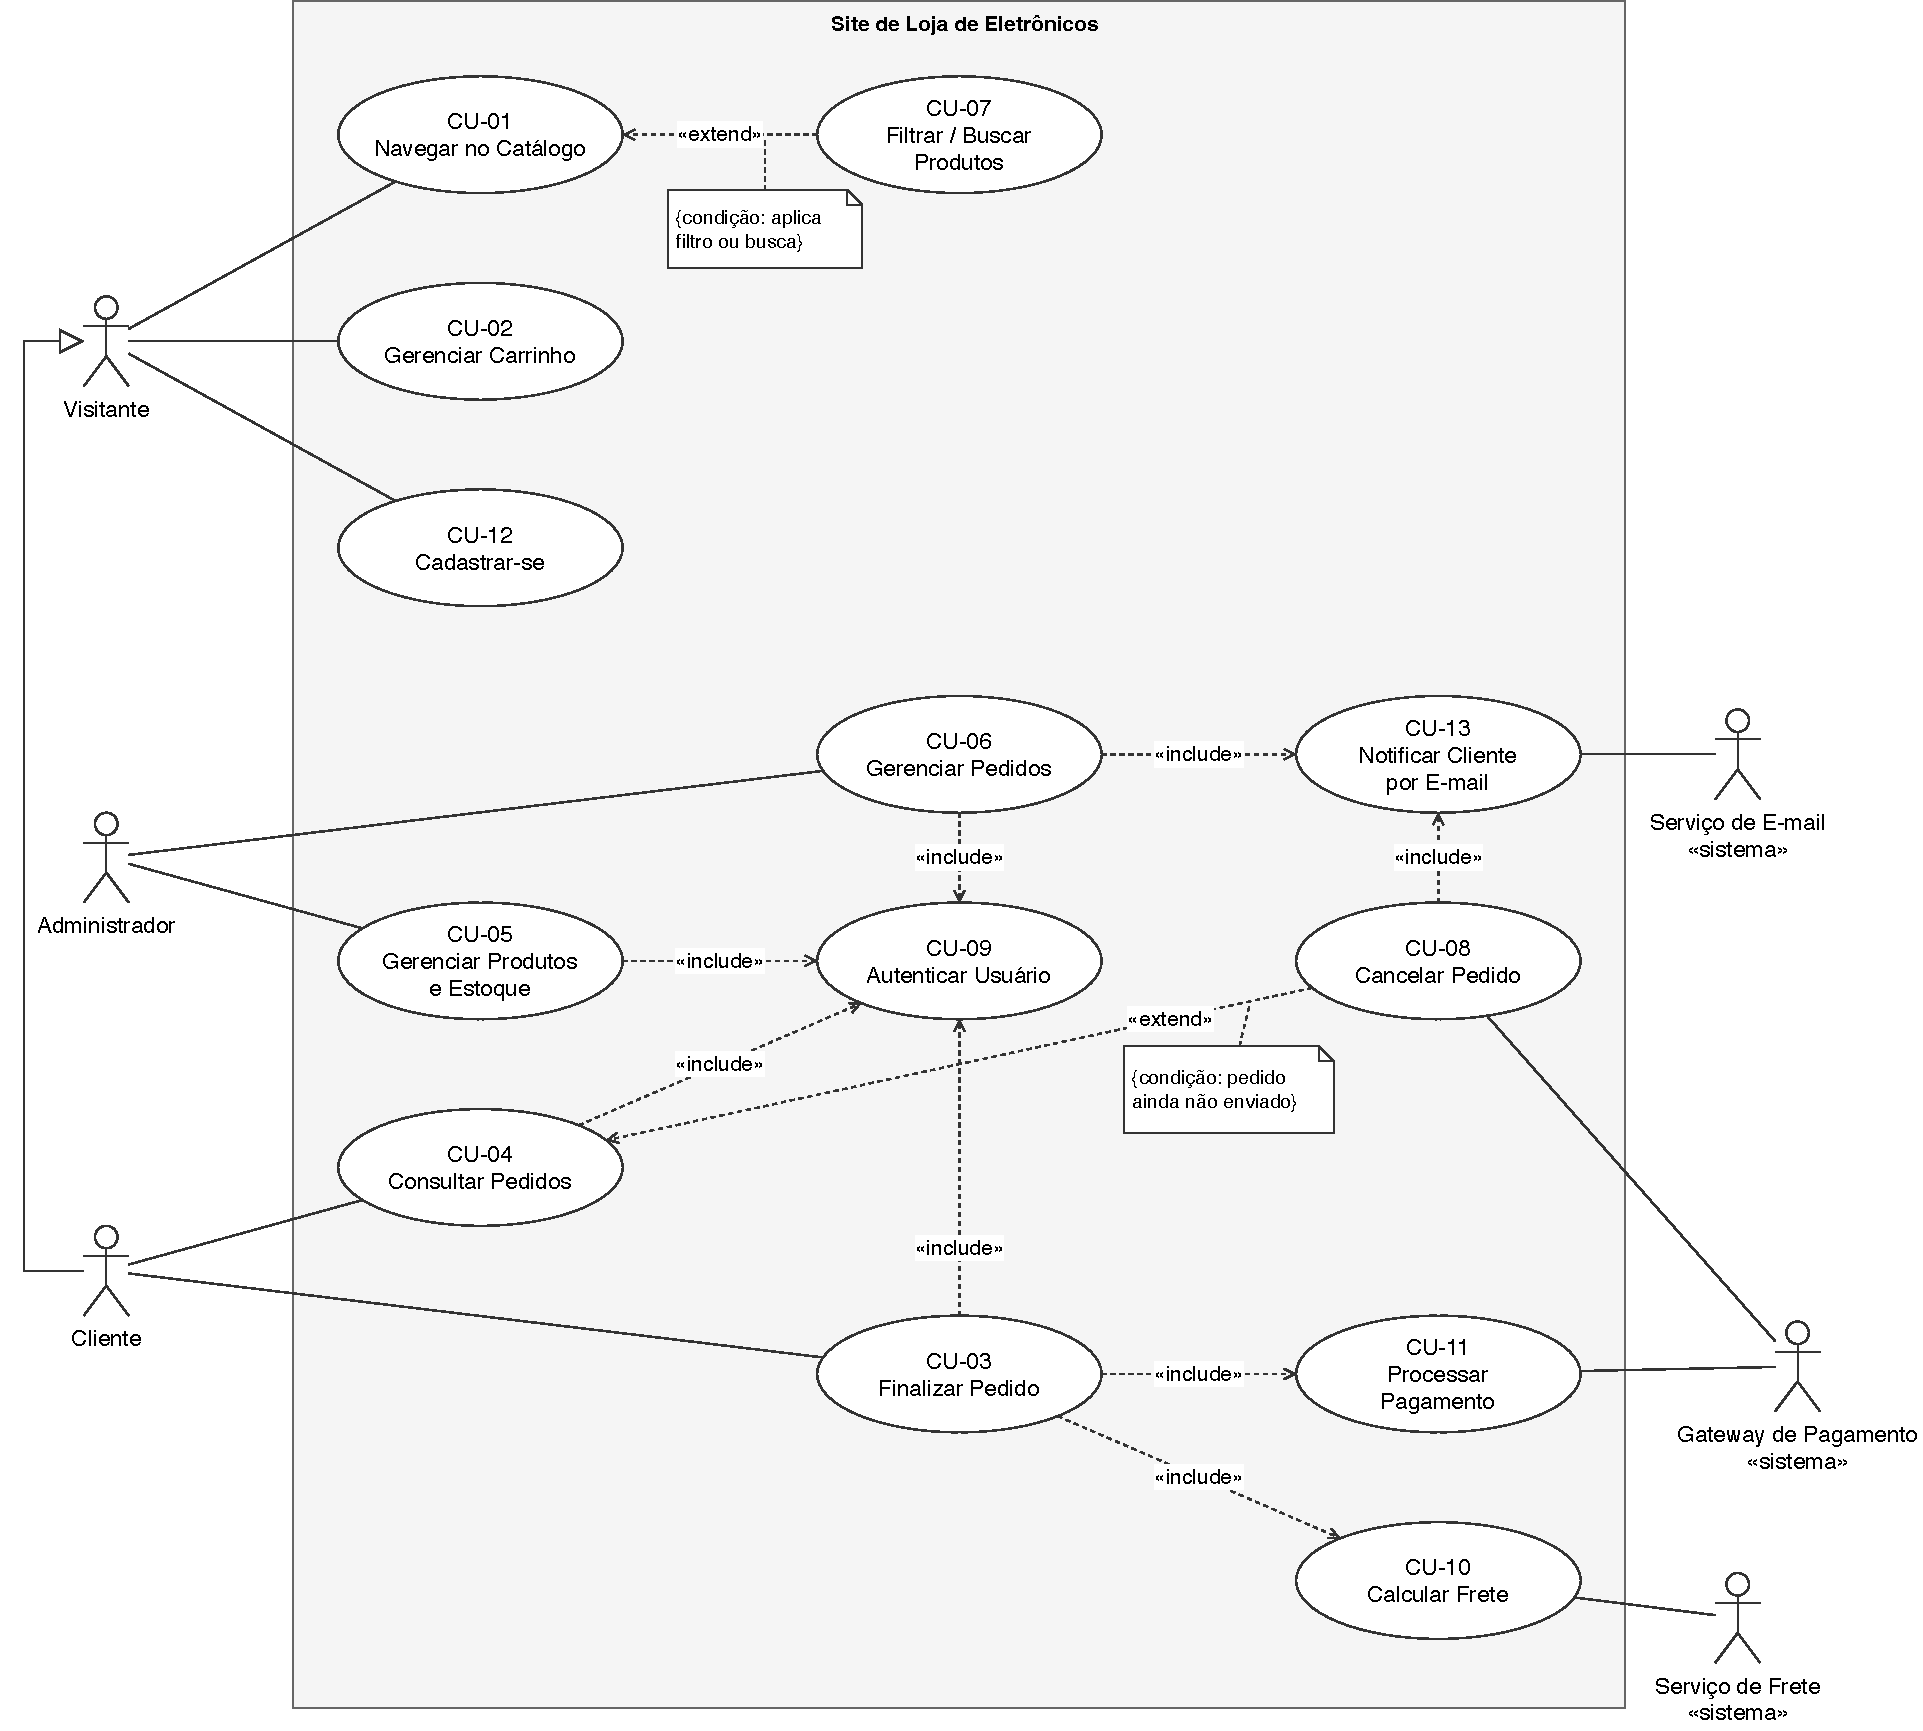
\includegraphics[trim=0.0bp 0.0bp 0.0bp 0.0bp, clip, width=192.2pt]{CU_CasosDeUso.pdf}};
  \hl{35.3}{92.8}{41.8}{103.9}{Principal}
  \hl{35.3}{144.4}{41.8}{155.5}{Principal}
  \hl{35.3}{185.7}{41.8}{196.7}{Principal}
  \hl{204.3}{195.3}{210.9}{206.3}{Apoio}
  \hl{198.3}{220.4}{204.9}{231.4}{Apoio}
  \hl{198.3}{134.1}{204.9}{145.1}{Apoio}
  \pcard{231.1889081455806}{64.0}{197.8110918544194}{55.0}{Principal}{Principais (à esquerda)}{Visitante, Cliente e Administrador: usam o sistema.}
  \pcard{231.1889081455806}{123.0}{197.8110918544194}{55.0}{Apoio}{Secundários (à direita)}{Gateway de Pagamento, Serviço de Frete e Serviço de E-mail: sistemas externos.}
  \pcard{231.1889081455806}{182.0}{197.8110918544194}{55.0}{Navy}{Cliente herda de Visitante}{Faz tudo o que o visitante faz, e finaliza e consulta pedidos.}
\end{tela}\end{frame}

% --- Carlos ---
\begin{frame}[plain]\begin{tela}
  \fundo{2.1}{LEITURA DO DIAGRAMA}{Como ler o diagrama de casos de uso}
    {As formas e as linhas dão o significado; as cores só agrupam}
  \fill[white] \pto{25}{64} rectangle \pto{223.1889081455806}{237};
  \draw[Borda, line width=0.5pt] \pto{25}{64} rectangle \pto{223.1889081455806}{237};
  \node[anchor=north west, inner sep=0pt] at \pto{28.0}{64.0} {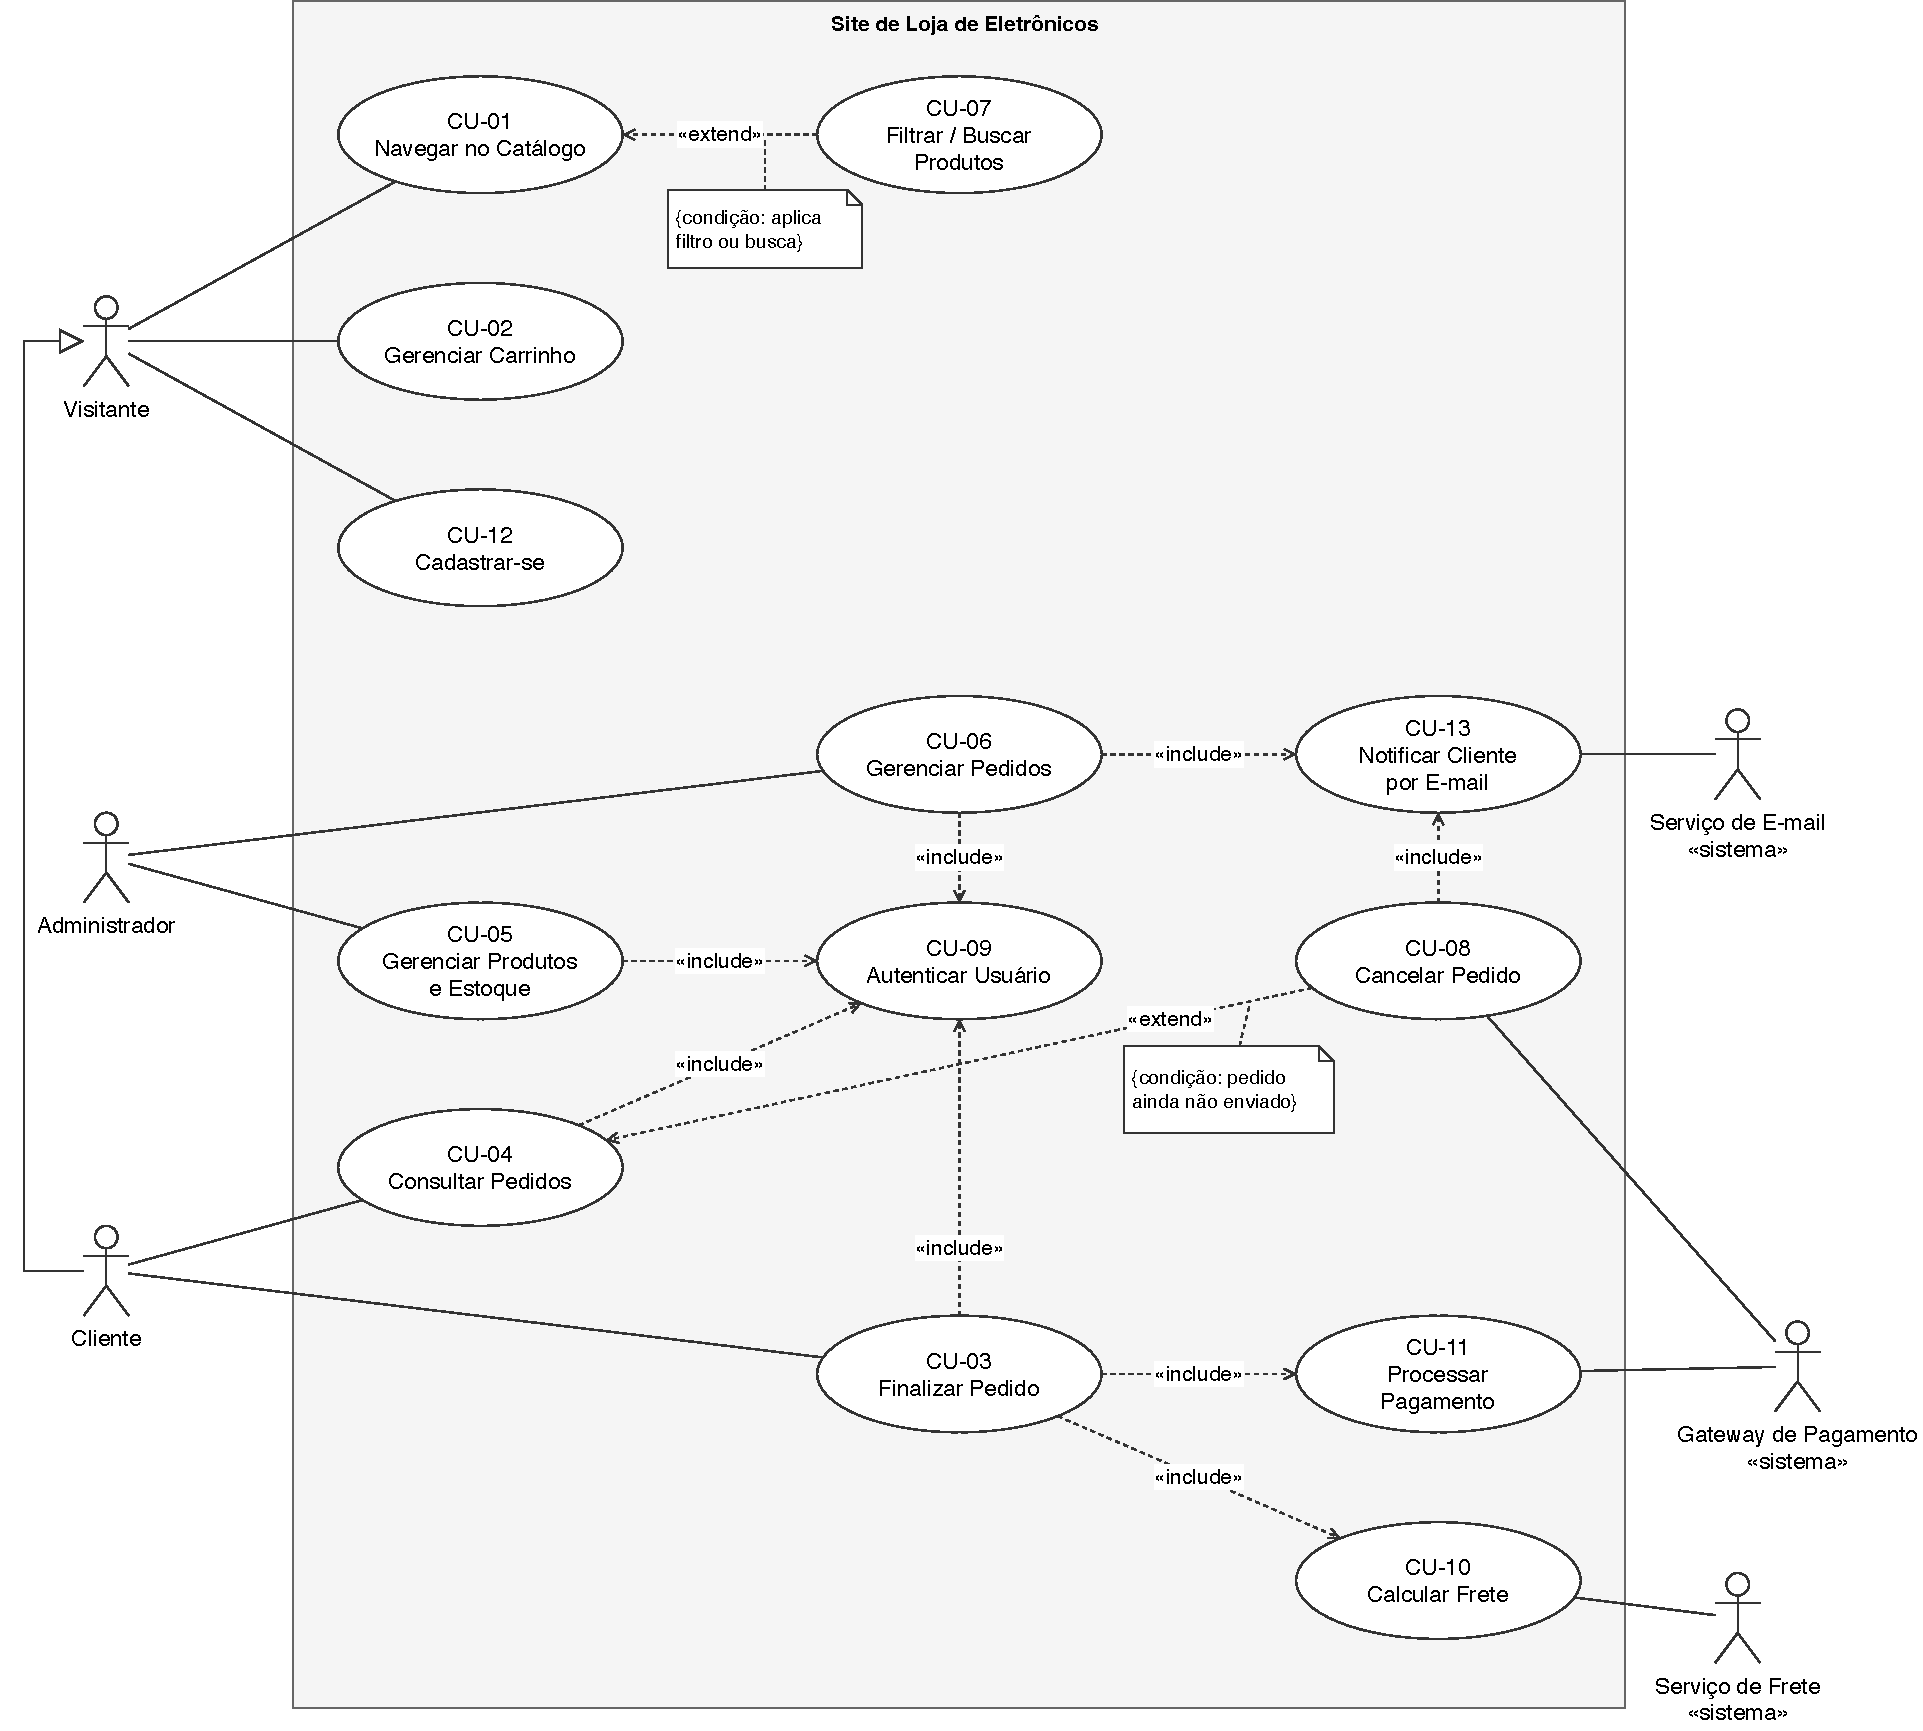
\includegraphics[trim=0.0bp 0.0bp 0.0bp 0.0bp, clip, width=192.2pt]{CU_CasosDeUso.pdf}};
  \mk{123.8}{71.0}{1}
  \mk{60.9}{71.0}{2}
  \mk{138.9}{71.0}{3}
  \mk{41.6}{98.3}{4}
  \pnum{231.1889081455806}{64.0}{197.8110918544194}{40.2}{1}{\textbf{Fronteira:} o retângulo é o sistema modelado.}
  \pnum{231.1889081455806}{108.2}{197.8110918544194}{40.2}{2}{\textbf{Azul:} os 7 casos principais, acionados por um ator.}
  \pnum{231.1889081455806}{152.5}{197.8110918544194}{40.2}{3}{\textbf{Amarelo:} os 6 casos de apoio, reutilizados ou condicionais.}
  \pnum{231.1889081455806}{196.8}{197.8110918544194}{40.2}{4}{\textbf{Linha contínua:} liga o ator aos casos em que participa.}
\end{tela}\end{frame}

% --- Carlos ---
\begin{frame}[plain]\begin{tela}
  \fundo{2.2}{DECISÕES DE MODELAGEM}{Seis decisões que dão forma ao diagrama}
    {Por que cada relacionamento foi escolhido (Seção 2.2)}
  \fill[white] \pto{25}{64} rectangle \pto{223.1889081455806}{237};
  \draw[Borda, line width=0.5pt] \pto{25}{64} rectangle \pto{223.1889081455806}{237};
  \node[anchor=north west, inner sep=0pt] at \pto{28.0}{64.0} {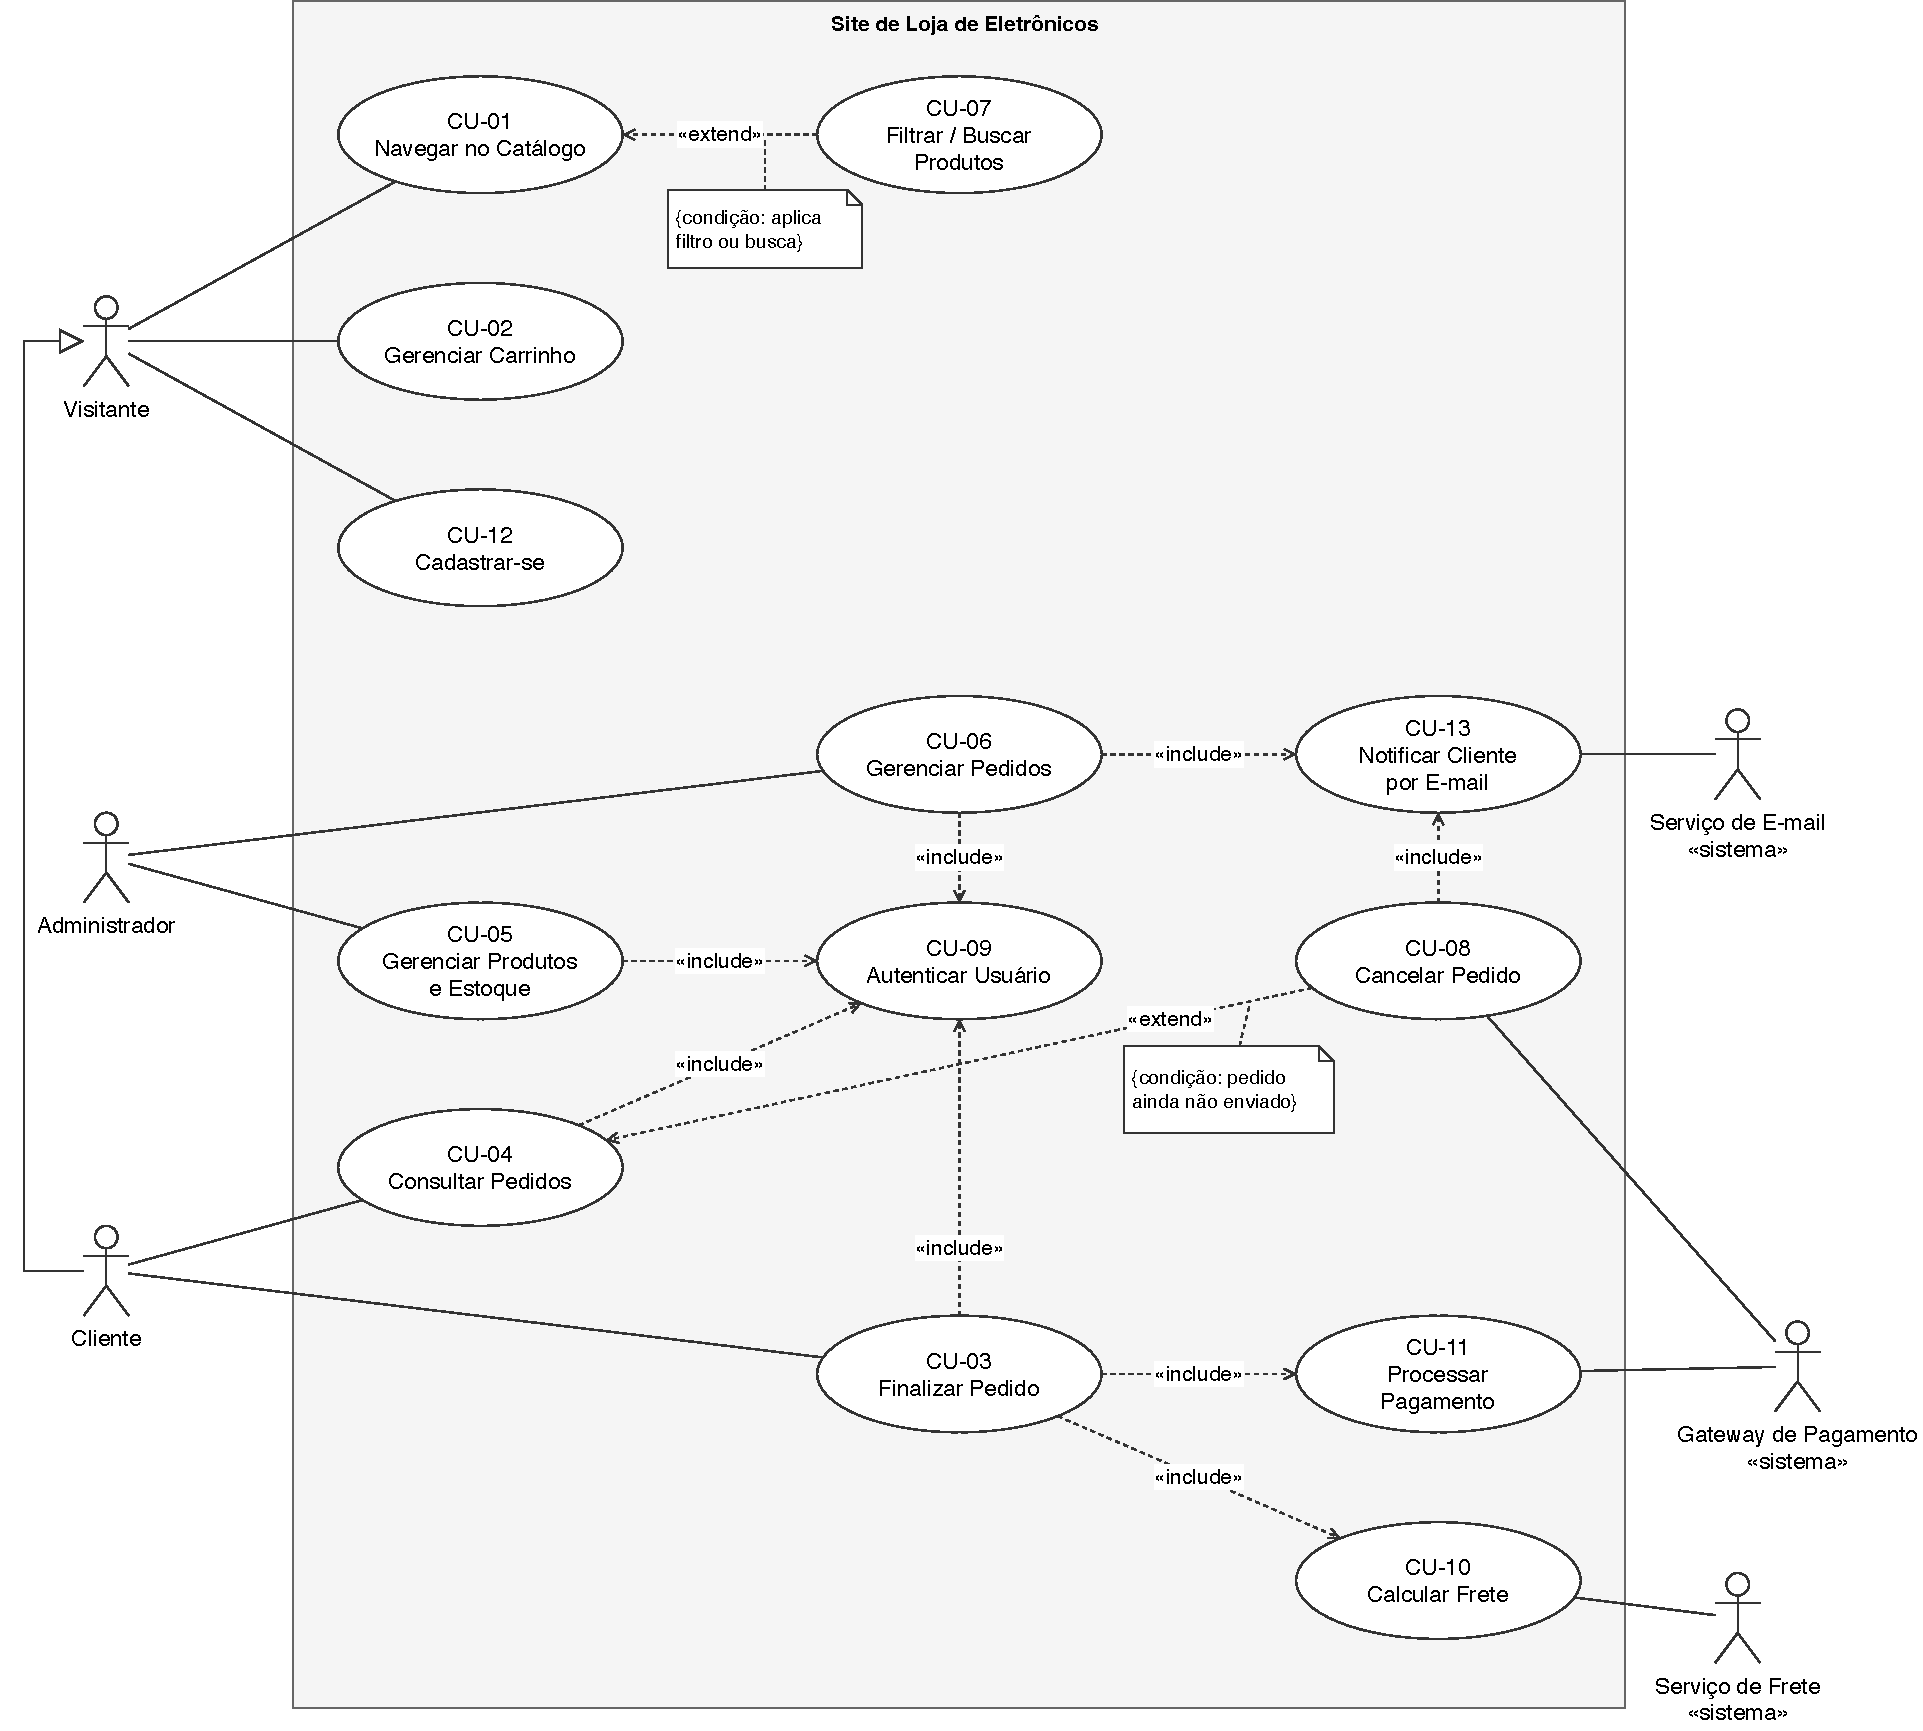
\includegraphics[trim=0.0bp 0.0bp 0.0bp 0.0bp, clip, width=192.2pt]{CU_CasosDeUso.pdf}};
  \mk{41.6}{191.2}{1}
  \mk{138.9}{153.6}{2}
  \mk{186.7}{194.9}{3}
  \mk{186.7}{153.6}{4}
  \mk{186.7}{132.9}{5}
  \mk{91.0}{112.3}{6}
  \pnum{231.1889081455806}{64.0}{197.8110918544194}{25.5}{1}{Cliente herda de Visitante.}
  \pnum{231.1889081455806}{93.5}{197.8110918544194}{25.5}{2}{Autenticar é um \inc\ reutilizado.}
  \pnum{231.1889081455806}{123.0}{197.8110918544194}{25.5}{3}{Frete e pagamento: \inc\ de Finalizar.}
  \pnum{231.1889081455806}{152.5}{197.8110918544194}{25.5}{4}{Filtrar e Cancelar: \ext.}
  \pnum{231.1889081455806}{182.0}{197.8110918544194}{25.5}{5}{Notificar é um caso à parte.}
  \pnum{231.1889081455806}{211.5}{197.8110918544194}{25.5}{6}{Cadastrar-se é do Visitante.}
\end{tela}\end{frame}

% --- Gabriel ---
\begin{frame}[plain]\begin{tela}
  \fundo{2.3}{RELACIONAMENTOS}{Quatro tipos de relacionamento}
    {Dois ligam ator e caso de uso; dois ligam casos de uso entre si (Tabela 2)}
  \fill[white] \pto{25}{64} rectangle \pto{223.1889081455806}{237};
  \draw[Borda, line width=0.5pt] \pto{25}{64} rectangle \pto{223.1889081455806}{237};
  \node[anchor=north west, inner sep=0pt] at \pto{28.0}{64.0} {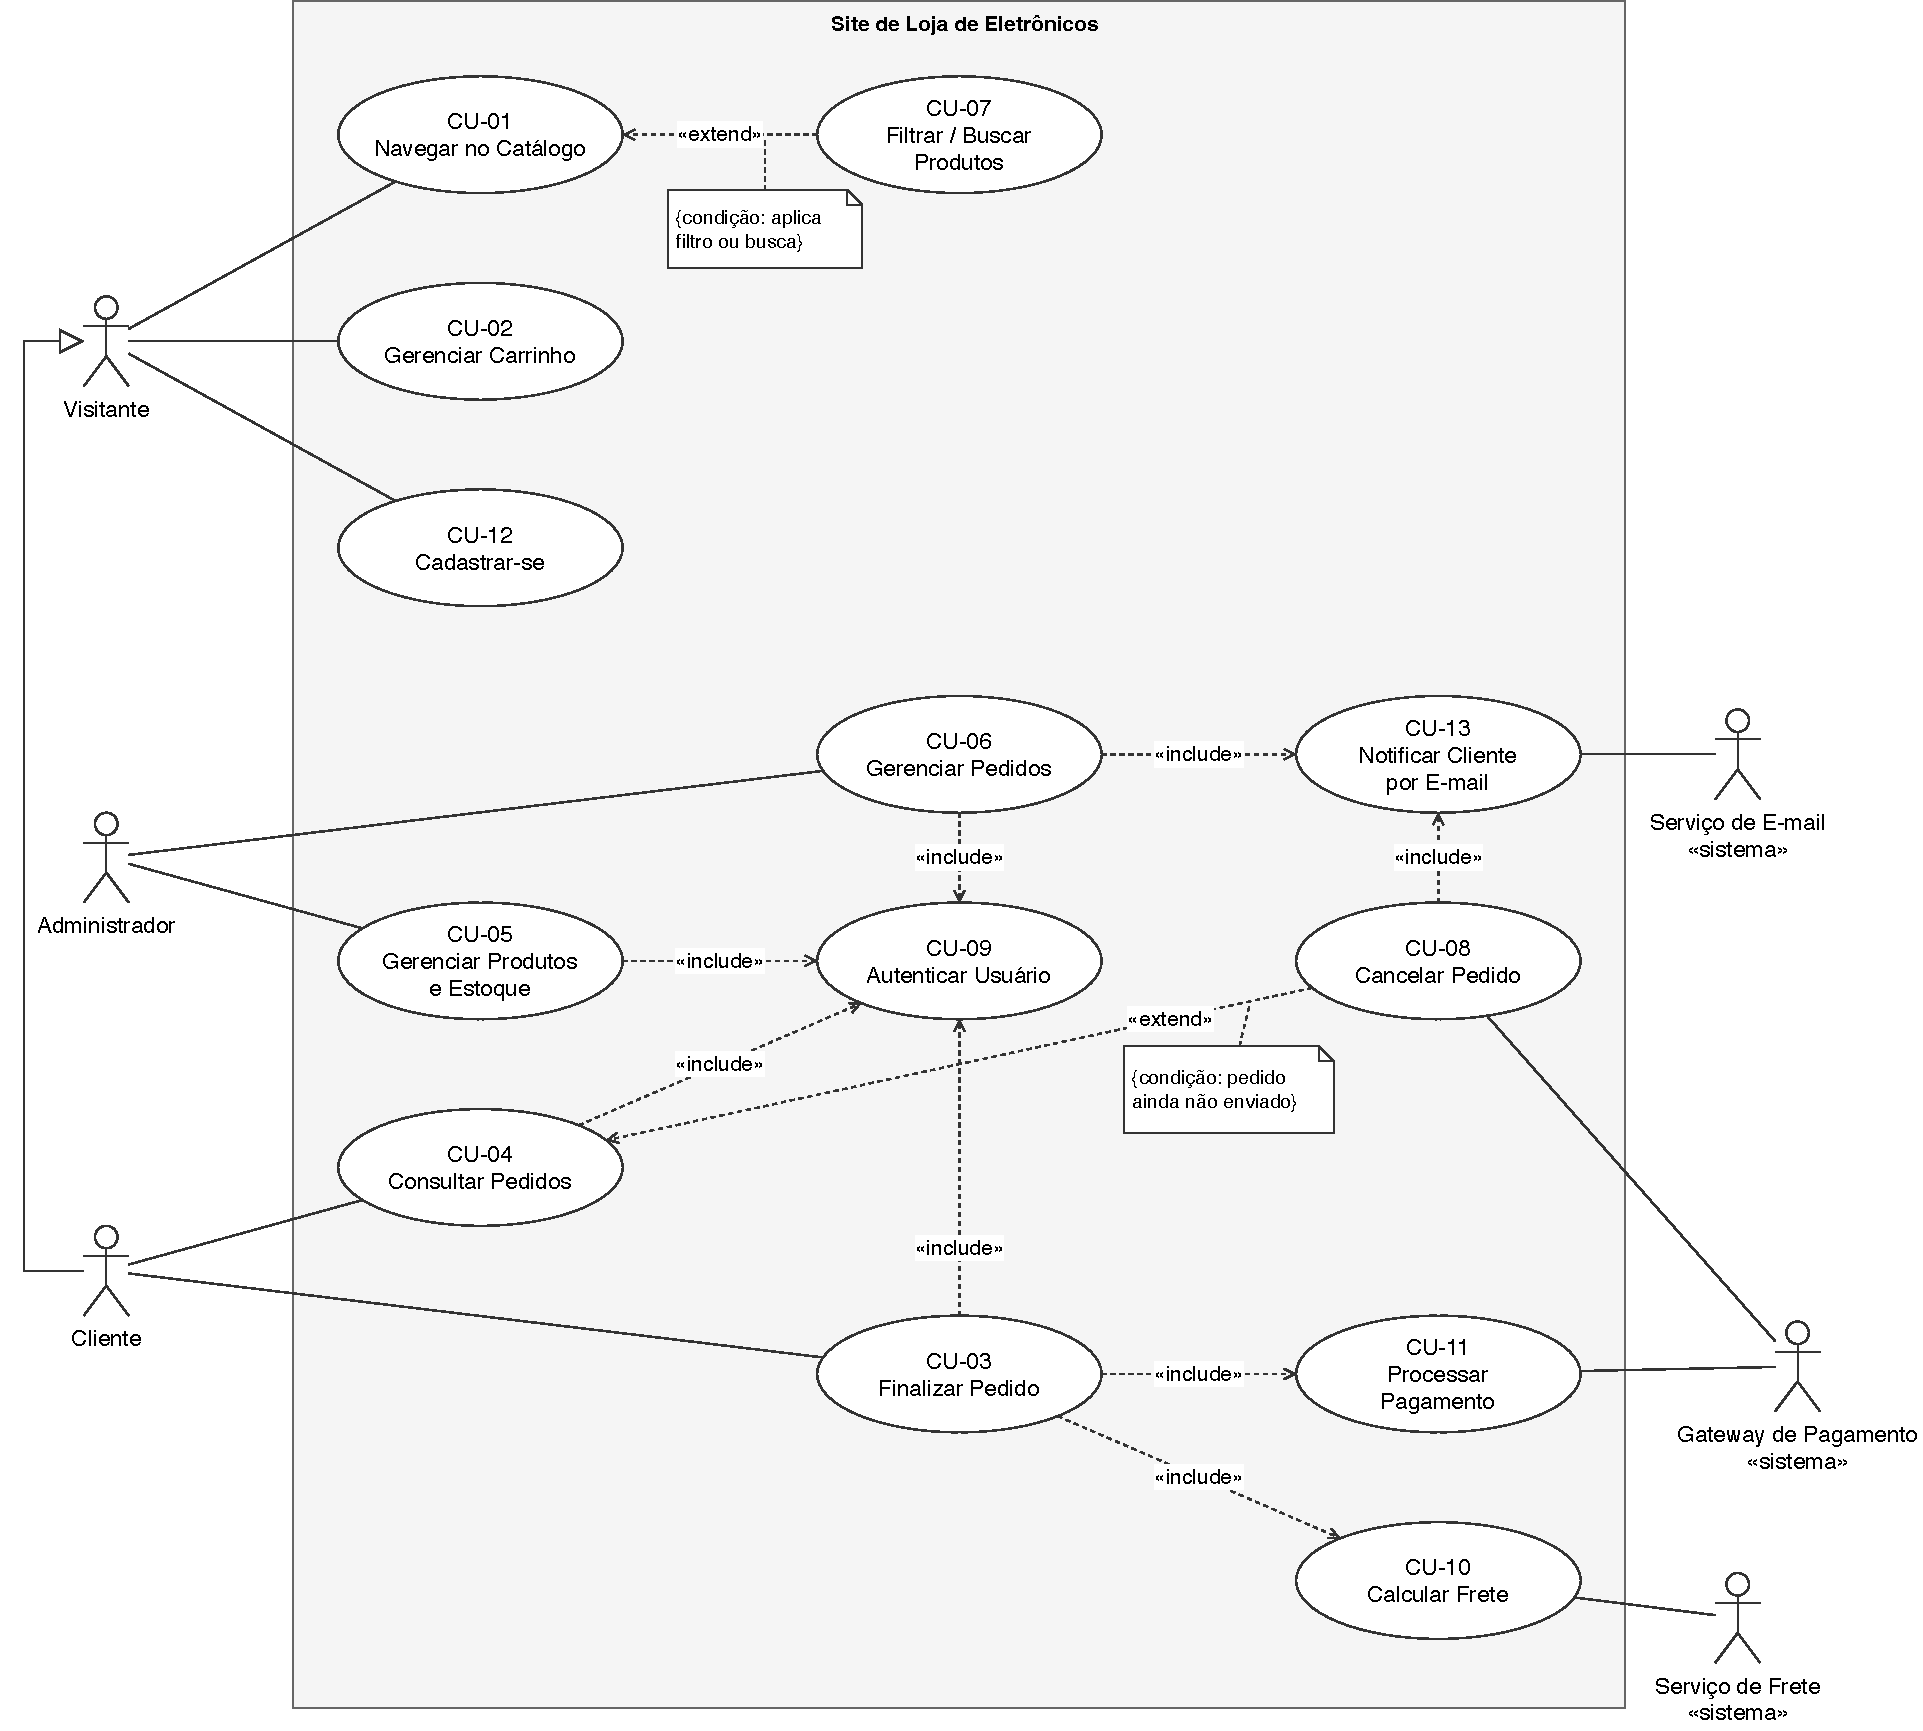
\includegraphics[trim=0.0bp 0.0bp 0.0bp 0.0bp, clip, width=192.2pt]{CU_CasosDeUso.pdf}};
  \mk{41.6}{93.0}{1}
  \mk{35.5}{191.2}{2}
  \mk{123.8}{153.6}{3}
  \mk{108.8}{71.0}{4}
  \pnum{231.1889081455806}{64.0}{197.8110918544194}{40.2}{1}{\textbf{Associação:} ator e caso de uso. Ex.: Visitante e CU-01.}
  \pnum{231.1889081455806}{108.2}{197.8110918544194}{40.2}{2}{\textbf{Generalização:} Cliente herda de Visitante.}
  \pnum{231.1889081455806}{152.5}{197.8110918544194}{40.2}{3}{\textbf{\inc:} sempre executa. Ex.: CU-03 inclui CU-09.}
  \pnum{231.1889081455806}{196.8}{197.8110918544194}{40.2}{4}{\textbf{\ext:} só com a condição da nota. Ex.: CU-07 em CU-01.}
\end{tela}\end{frame}

% --- Gabriel ---
\begin{frame}[plain]\begin{tela}
  \fundo{2.3}{RELACIONAMENTOS NO DIAGRAMA}{Oito \inc\ e dois \ext}
    {Cada relacionamento do diagrama, na direção da seta (Tabela 3)}
  \fill[white] \pto{25}{64} rectangle \pto{223.1889081455806}{237};
  \draw[Borda, line width=0.5pt] \pto{25}{64} rectangle \pto{223.1889081455806}{237};
  \node[anchor=north west, inner sep=0pt] at \pto{28.0}{64.0} {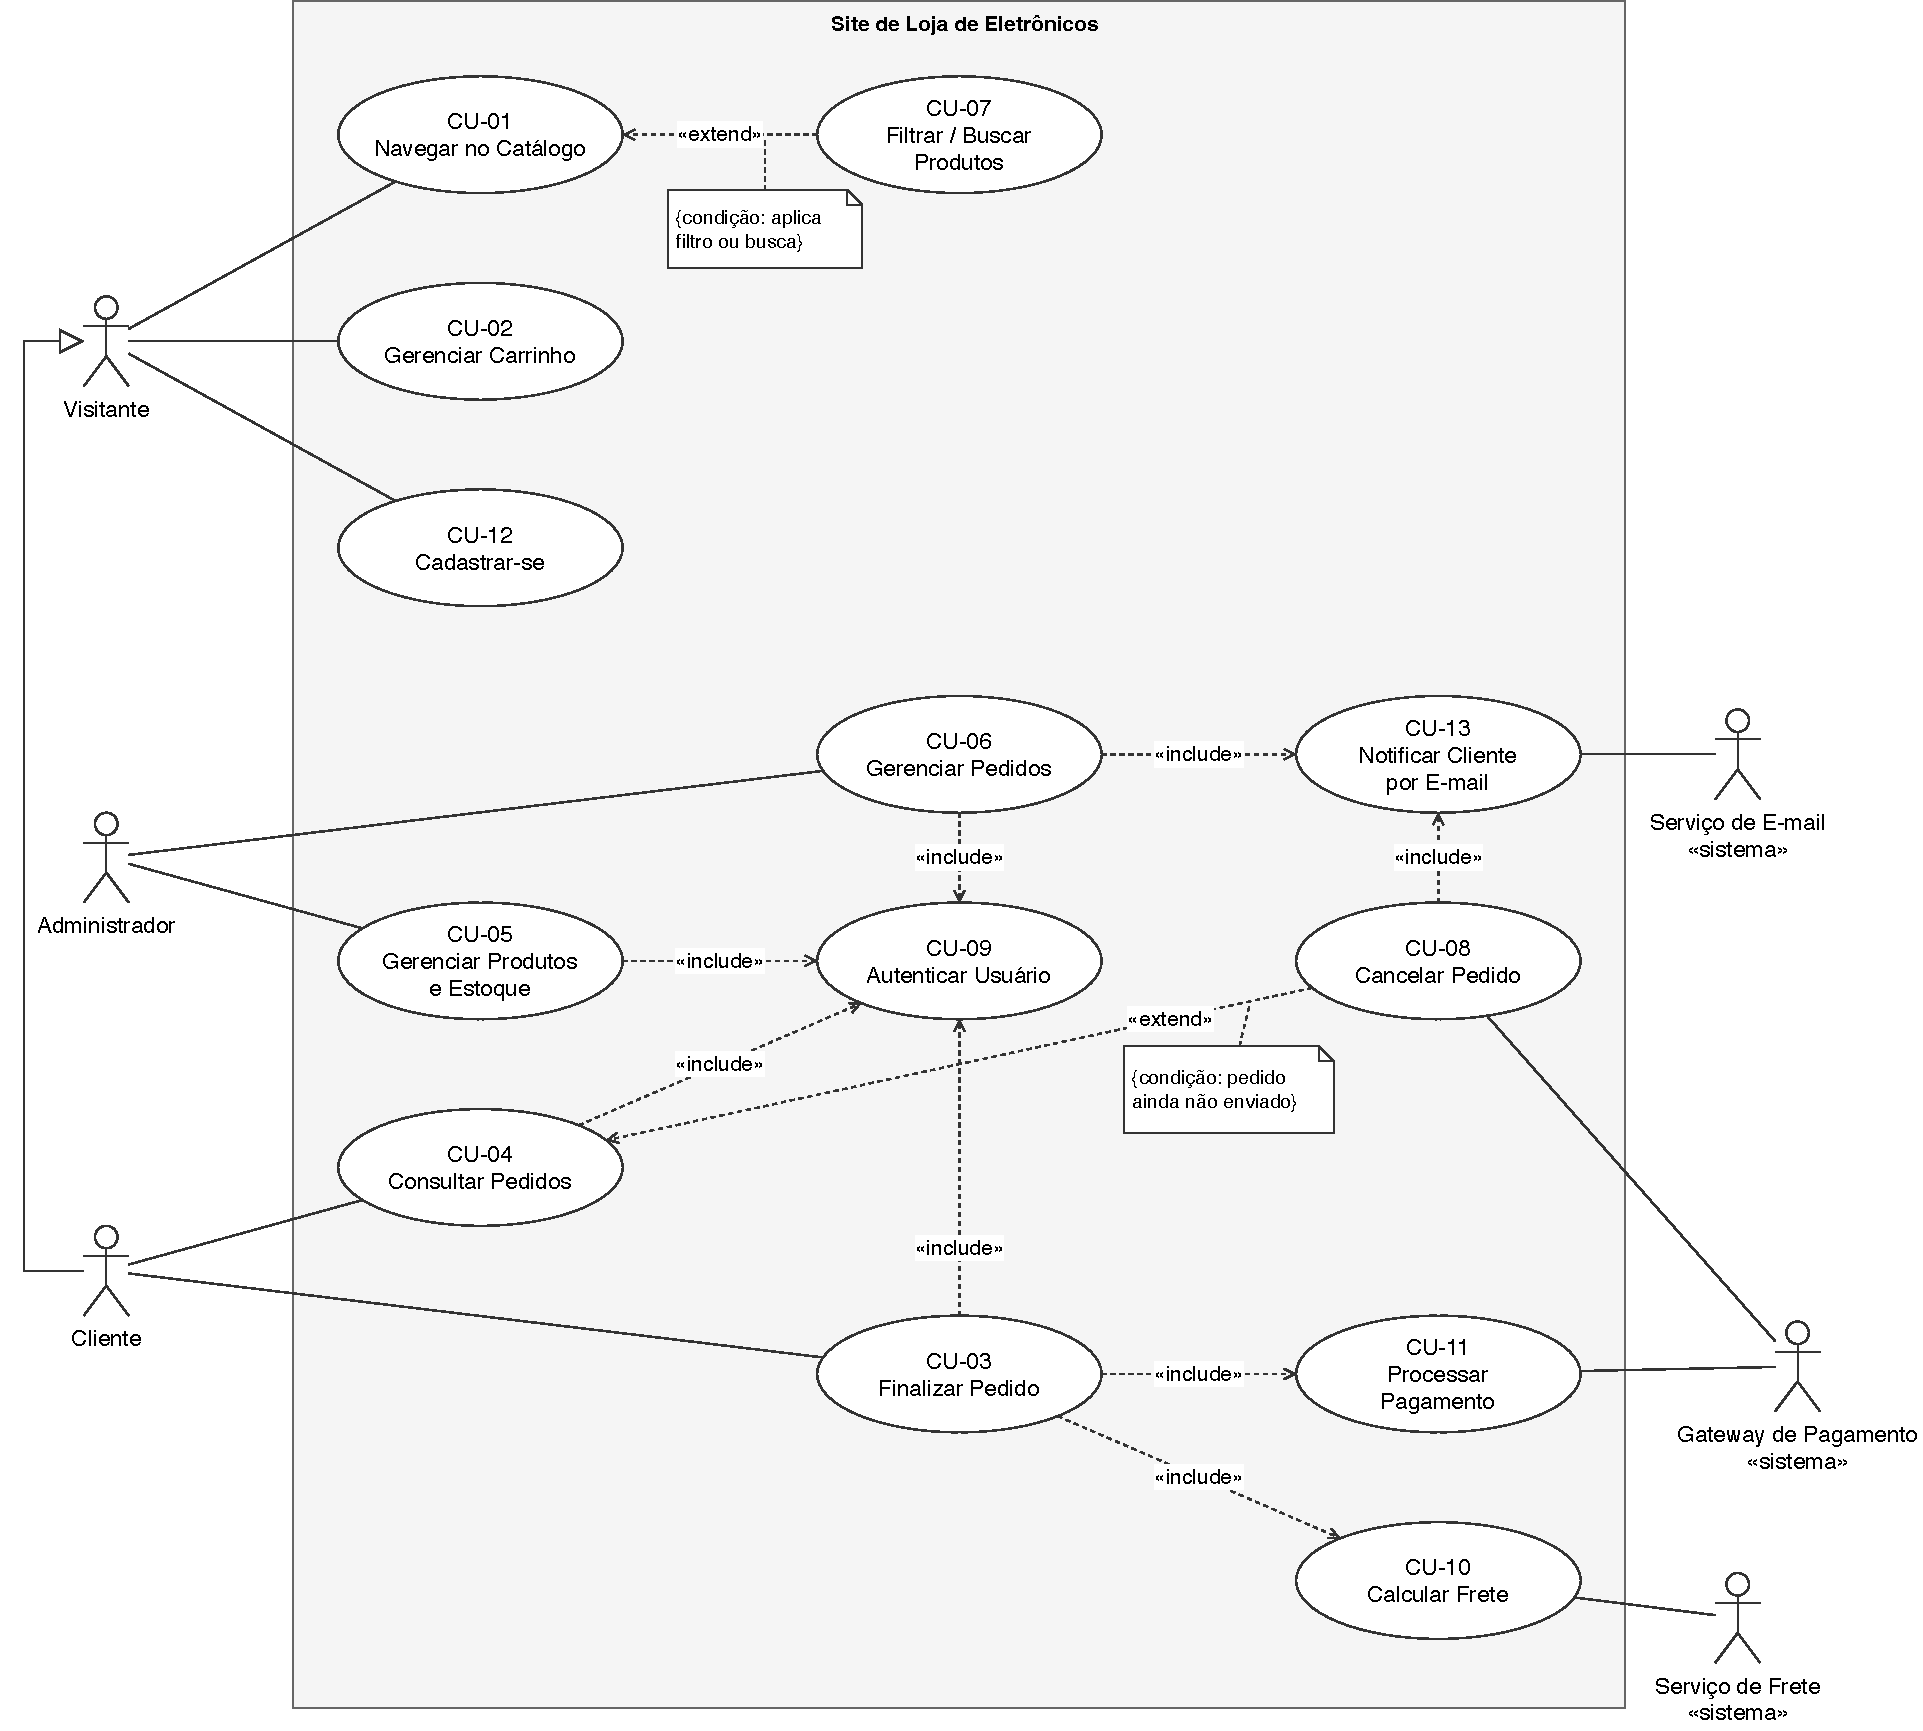
\includegraphics[trim=0.0bp 0.0bp 0.0bp 0.0bp, clip, width=192.2pt]{CU_CasosDeUso.pdf}};
  \hl{108.6}{153.4}{139.1}{167.1}{Principal}
  \hl{156.4}{132.7}{186.9}{146.5}{Principal}
  \hl{60.7}{70.8}{91.2}{84.6}{Apoio}
  \hl{60.7}{174.0}{91.2}{187.8}{Apoio}
  \pcard{231.1889081455806}{64.0}{197.8110918544194}{66.0}{Principal}{8 \inc\ (obrigatório)}{CU-03 inclui CU-09, 10 e 11. CU-04, 05 e 06 incluem CU-09. CU-06 e CU-08 incluem CU-13.}
  \pcard{231.1889081455806}{134.0}{197.8110918544194}{58.0}{Apoio}{2 \ext\ (condicional)}{CU-07 estende CU-01, com filtro ou busca. CU-08 estende CU-04, se o pedido não foi enviado.}
  \pcard{231.1889081455806}{196.0}{197.8110918544194}{41.0}{Navy}{Sentido da seta}{O \inc\ sai de quem inclui; o \ext\ sai da extensão para o caso base.}
\end{tela}\end{frame}

% --- Gabriel ---
\begin{frame}[plain]\begin{tela}
  \fundo{2.4}{ESPECIFICAÇÃO · CU-01 · CU-02}{Navegar no catálogo e montar o carrinho}
    {Os casos de entrada do Visitante (Tabelas 4 e 5)}
  \fill[white] \pto{25}{64} rectangle \pto{210}{237};
  \draw[Borda, line width=0.5pt] \pto{25}{64} rectangle \pto{210}{237};
  \node[anchor=north west, inner sep=0pt] at \pto{25.0}{64.0} {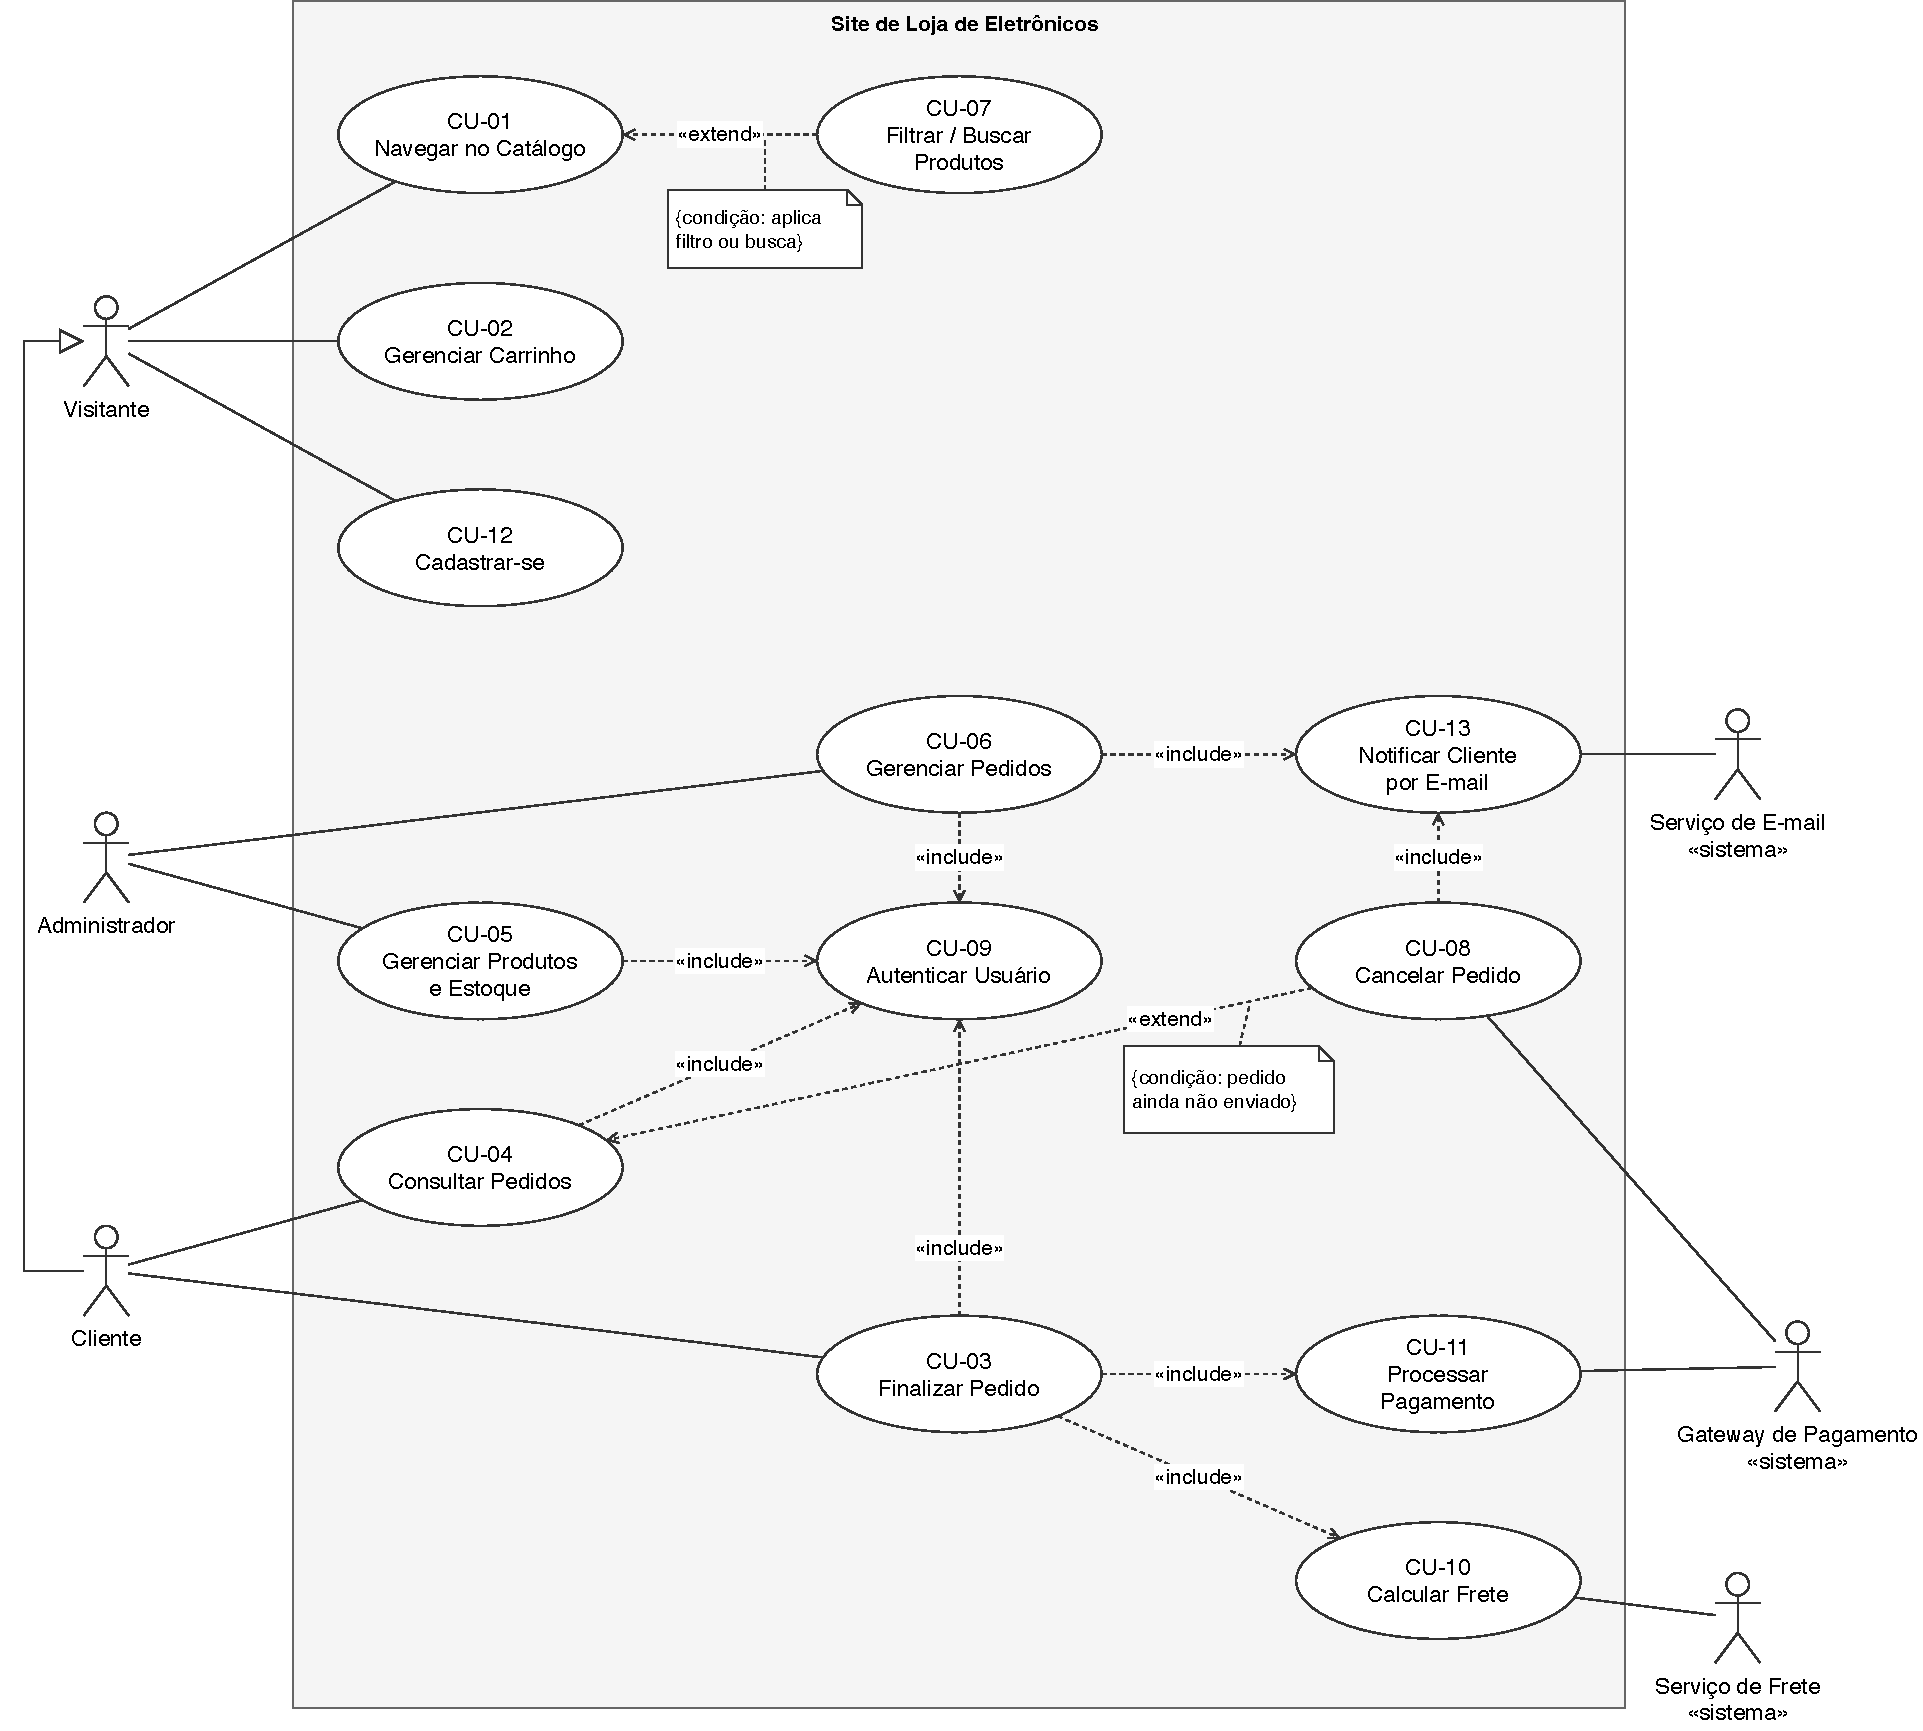
\includegraphics[trim=17.9bp 332.9bp 372.6bp 0.0bp, clip, width=185.0pt]{CU_CasosDeUso.pdf}};
  \hl{73.3}{75.4}{124.2}{98.3}{Destaque}
  \hl{73.3}{109.8}{124.2}{132.7}{Destaque}
  \hl{153.2}{75.4}{204.1}{98.3}{Navy}
  \pcu{218.0}{64.0}{211.0}{80.8}{Principal}{CU-01 Navegar no Catálogo}
    {\textbf{Ator:} Visitante. \textbf{Pré:} nenhuma.}
    {1. Acessa o catálogo.\par 2. Sistema lista os produtos ativos.\par 3. Abre um produto.\par 4. Sistema mostra detalhes e estoque.}
    {\textbf{A1} Filtro ou busca: CU-07.\par \textbf{A2} Sem resultado: limpar filtros.}
  \pcu{218.0}{148.8}{211.0}{88.2}{Principal}{CU-02 Gerenciar Carrinho}
    {\textbf{Atores:} Visitante e Cliente. \textbf{Pré:} produto disponível.}
    {1. Adiciona produto e quantidade.\par 2. Sistema confere o estoque.\par 3. Atualiza carrinho e subtotal.\par 4. Altera ou remove itens.\par 5. Segue para o CU-03.}
    {\textbf{A1} Ao entrar, itens vão para a conta.\par \textbf{E1 · E2} Acima do estoque; item indisponível.}
\end{tela}\end{frame}

% --- Gabriel ---
\begin{frame}[plain]\begin{tela}
  \fundo{2.4}{ESPECIFICAÇÃO · CU-03}{CU-03: só existe pedido com frete e pagamento}
    {Inclui o CU-09, o CU-10 e o CU-11 (Tabela 6)}
  \fill[white] \pto{25}{64} rectangle \pto{260}{237};
  \draw[Borda, line width=0.5pt] \pto{25}{64} rectangle \pto{260}{237};
  \node[anchor=north west, inner sep=0pt] at \pto{25.0}{64.0} {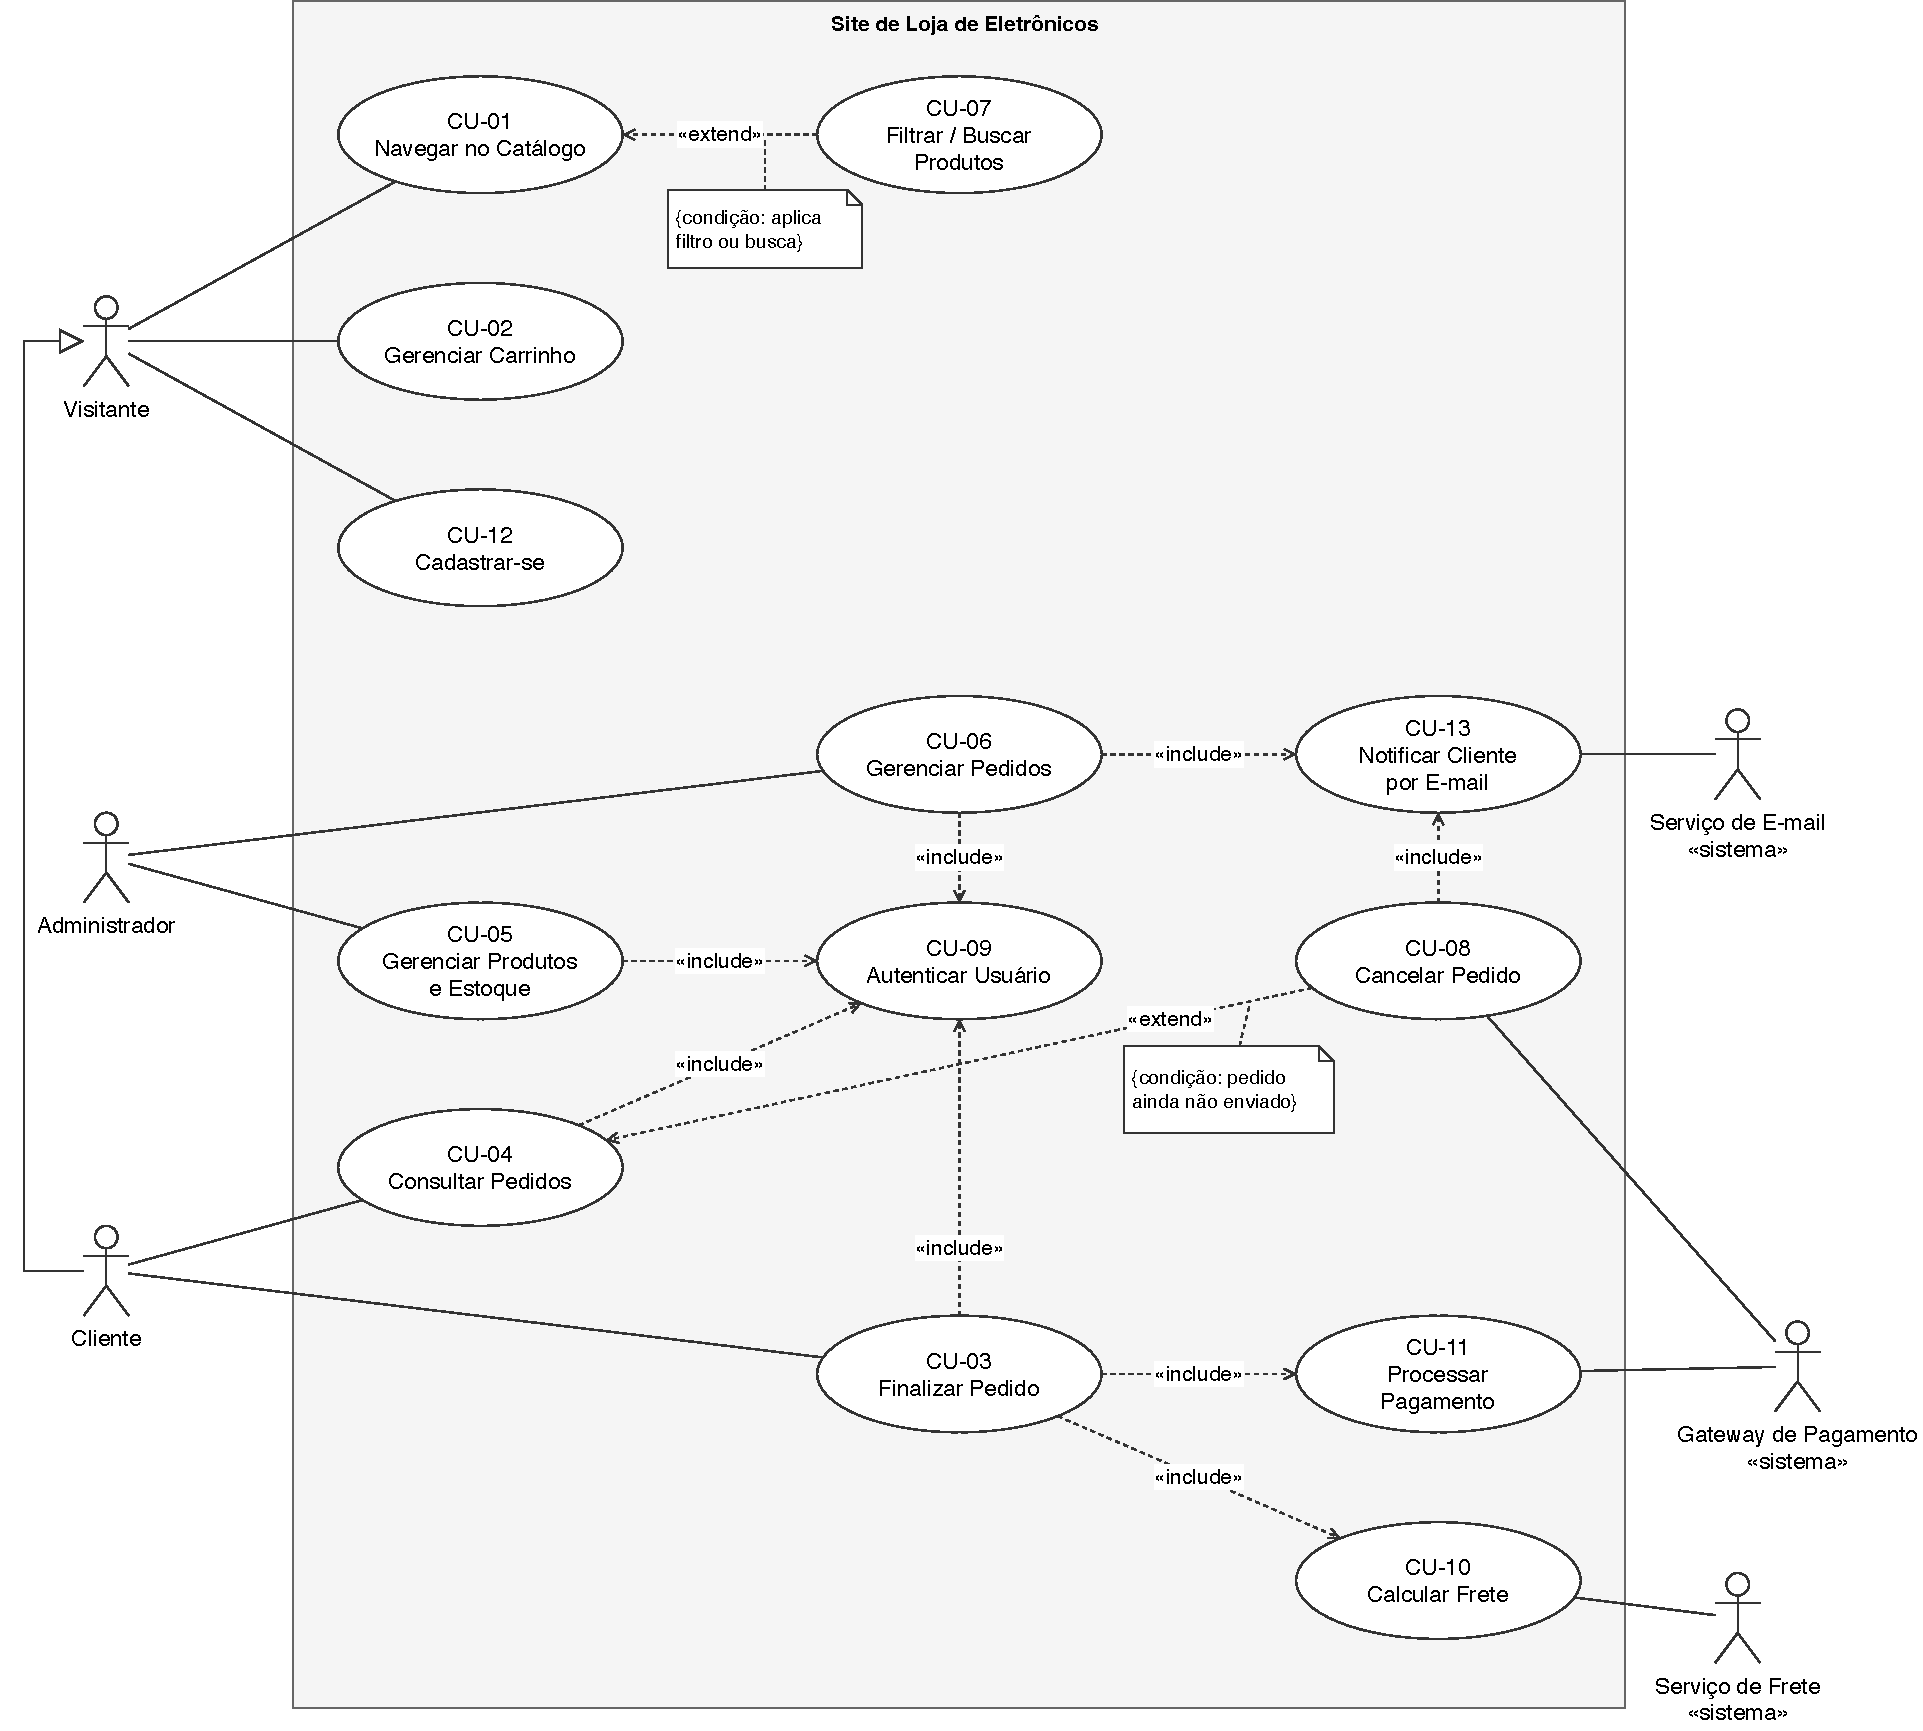
\includegraphics[trim=17.9bp 0.0bp 142.7bp 269.6bp, clip, width=235.0pt]{CU_CasosDeUso.pdf}};
  \hl{138.7}{174.3}{183.9}{194.7}{Destaque}
  \hl{138.7}{113.2}{183.9}{133.6}{Navy}
  \hl{209.6}{204.9}{254.8}{225.2}{Navy}
  \hl{209.6}{174.3}{254.8}{194.7}{Navy}
  \pcu{268.0}{64.0}{161.0}{173.0}{Principal}{CU-03 Finalizar Pedido}
    {\textbf{Ator:} Cliente. \textbf{Pré:} carrinho com itens.}
    {1. Autentica-se (CU-09).\par 2. Informa o endereço.\par 3. Sistema busca o frete (CU-10).\par 4. Escolhe o frete.\par 5. Escolhe o pagamento.\par 6. Confirma o resumo.\par 7. Sistema reserva estoque e cria o pedido.\par 8. Cobrança no gateway (CU-11).\par 9. Pedido pago.}
    {\textbf{A1} Pix ou boleto aguardam confirmação.\par \textbf{E1} Recusado: outra forma.\par \textbf{E2} Sem estoque: ajusta.\par \textbf{E3} Sem frete: não avança.}
\end{tela}\end{frame}

% --- Gabriel ---
\begin{frame}[plain]\begin{tela}
  \fundo{2.4}{ESPECIFICAÇÃO · CU-04 · CU-05}{Consultar pedidos e gerenciar produtos}
    {O Cliente acompanha os pedidos; o Administrador cuida do catálogo (Tabelas 7 e 8)}
  \fill[white] \pto{25}{64} rectangle \pto{210}{237};
  \draw[Borda, line width=0.5pt] \pto{25}{64} rectangle \pto{210}{237};
  \node[anchor=north west, inner sep=0pt] at \pto{25.0}{64.0} {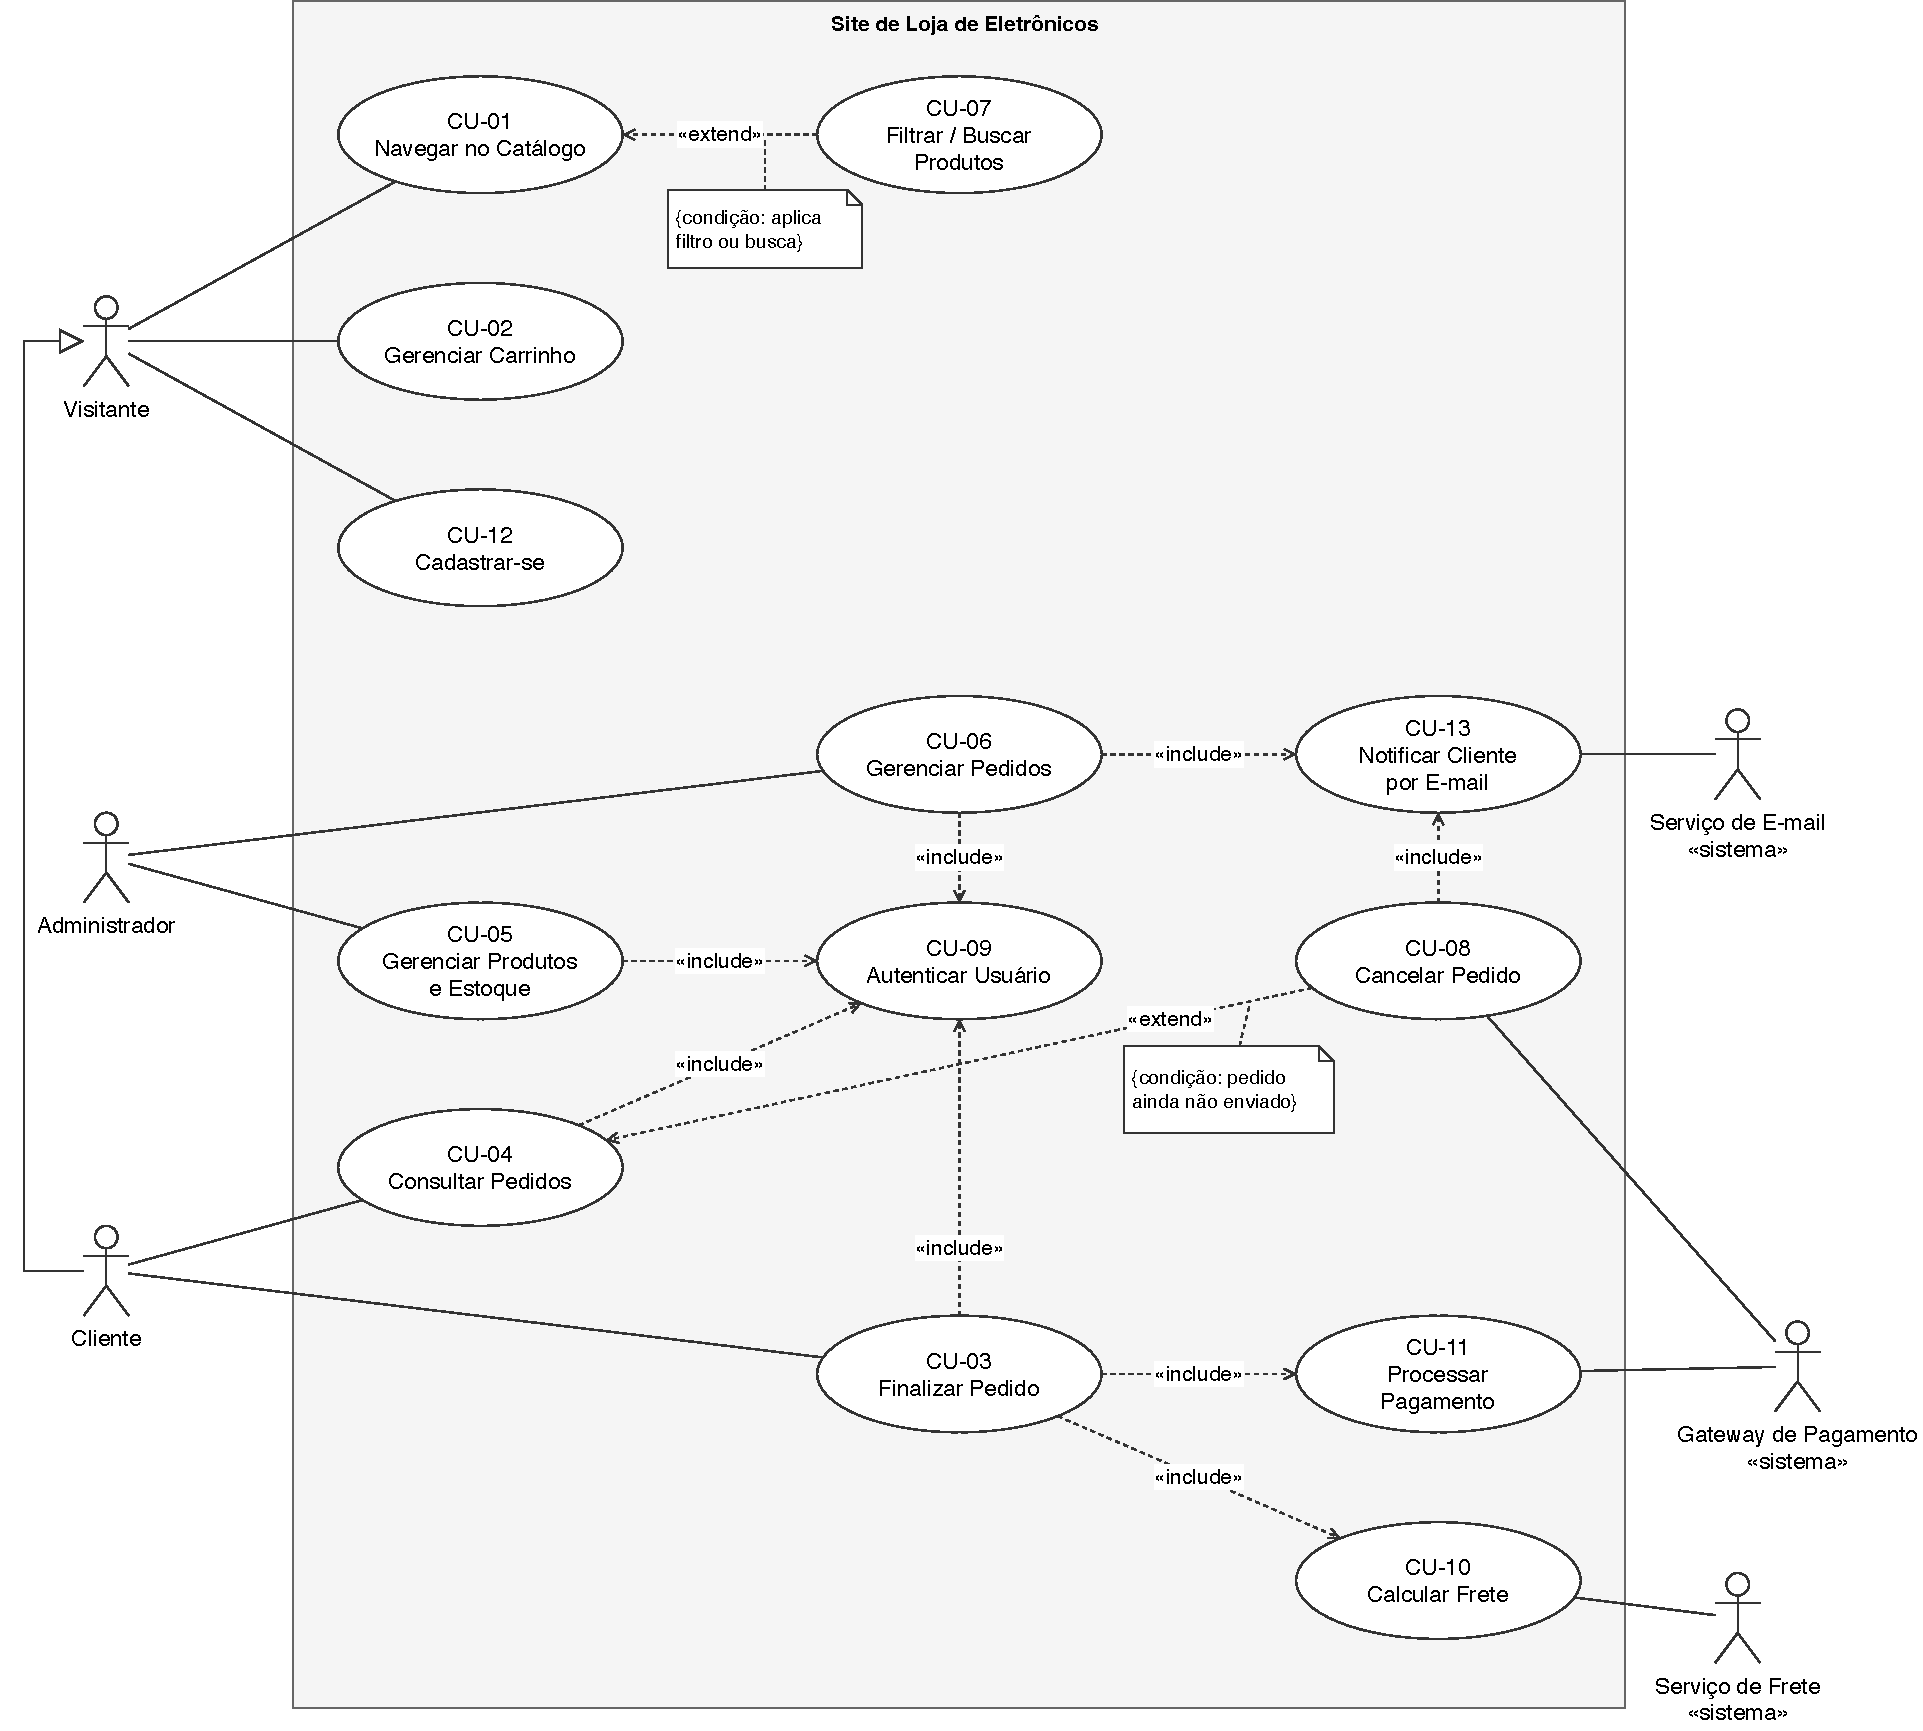
\includegraphics[trim=17.9bp 70.0bp 372.6bp 262.8bp, clip, width=185.0pt]{CU_CasosDeUso.pdf}};
  \hl{73.3}{156.3}{124.2}{179.2}{Destaque}
  \hl{73.3}{121.8}{124.2}{144.7}{Destaque}
  \hl{153.2}{121.8}{204.1}{144.7}{Navy}
  \pcu{218.0}{64.0}{211.0}{84.5}{Principal}{CU-04 Consultar Pedidos}
    {\textbf{Ator:} Cliente. \textbf{Pré:} ao menos um pedido.}
    {1. Autentica-se (CU-09).\par 2. Abre ``Meus Pedidos''.\par 3. Sistema lista os pedidos.\par 4. Abre um pedido.\par 5. Vê itens e histórico.}
    {\textbf{A1} Cancelar: CU-08.\par \textbf{E1} Pedido de outro cliente: negado.}
  \pcu{218.0}{152.5}{211.0}{84.5}{Principal}{CU-05 Produtos e Estoque}
    {\textbf{Ator:} Administrador. \textbf{Pré:} conta de admin.}
    {1. Autentica-se (CU-09).\par 2. Cadastra ou edita produto.\par 3. Sistema valida e publica.\par 4. Ajusta o estoque.\par 5. Sistema atualiza.}
    {\textbf{A1 · A2} Inativar; nova categoria ou marca.\par \textbf{E1 · E2} Dados inválidos; estoque negativo.}
\end{tela}\end{frame}

% --- Gabriel ---
\begin{frame}[plain]\begin{tela}
  \fundo{2.4}{ESPECIFICAÇÃO · CU-06}{CU-06: o administrador conduz o pedido}
    {Cada mudança de status avisa o cliente pelo CU-13 (Tabela 9)}
  \fill[white] \pto{25}{64} rectangle \pto{260}{237};
  \draw[Borda, line width=0.5pt] \pto{25}{64} rectangle \pto{260}{237};
  \node[anchor=north west, inner sep=0pt] at \pto{25.0}{64.0} {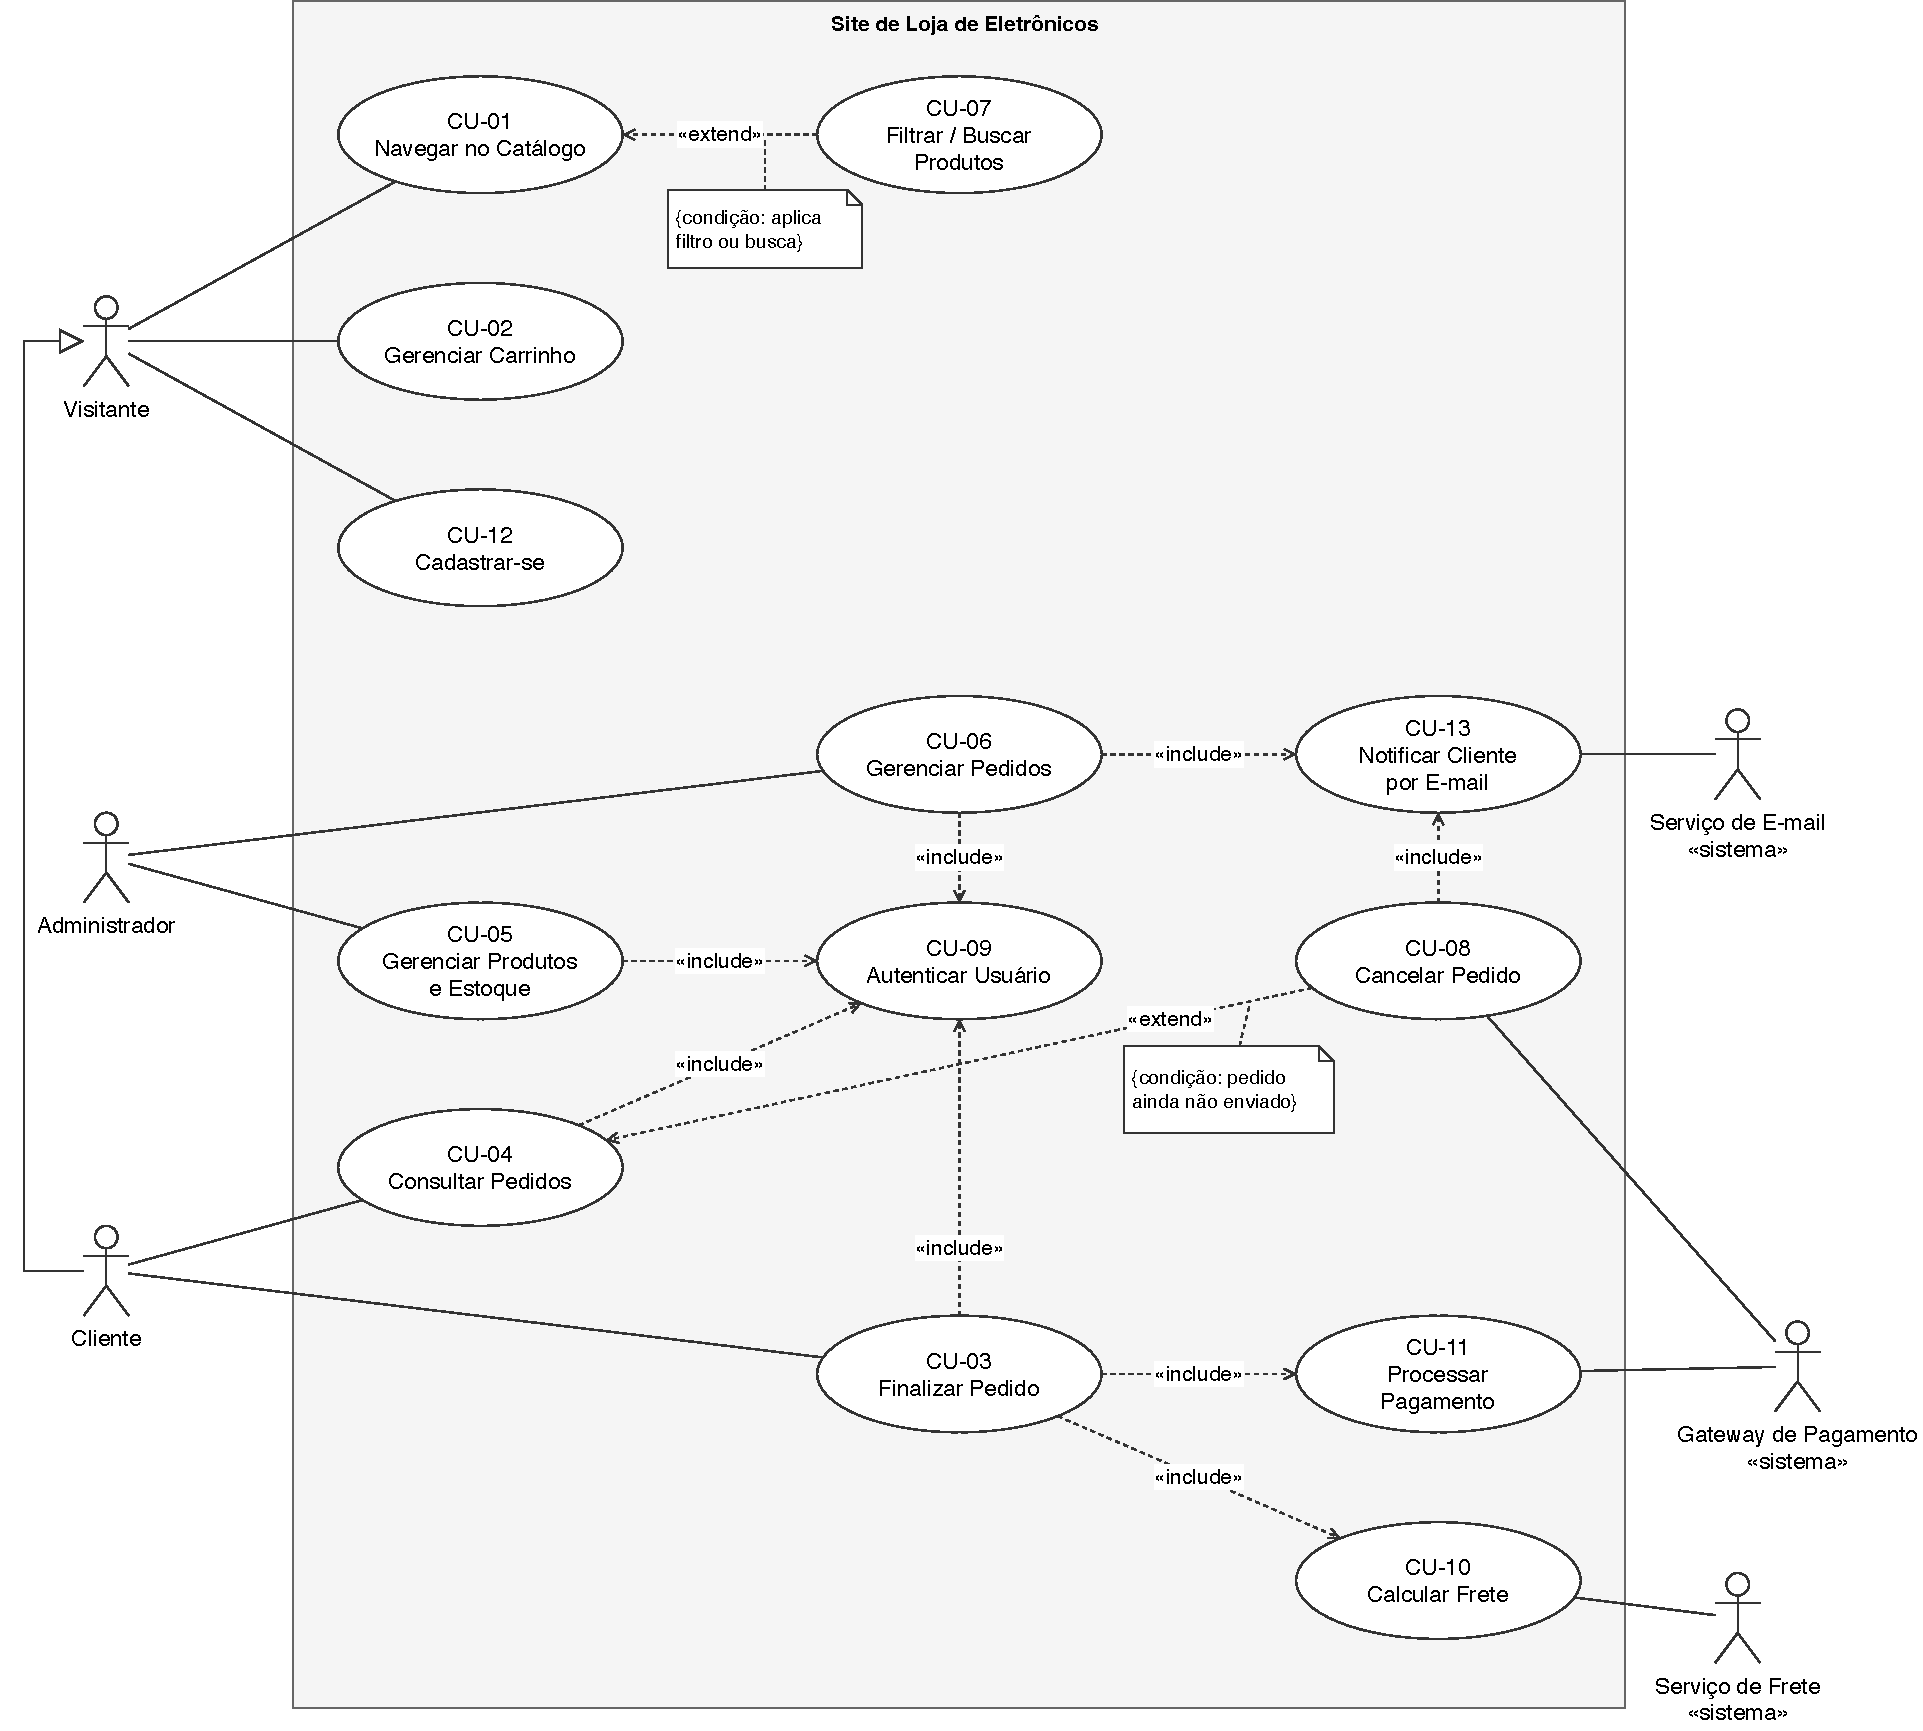
\includegraphics[trim=17.9bp 137.5bp 142.7bp 132.1bp, clip, width=235.0pt]{CU_CasosDeUso.pdf}};
  \hl{138.7}{125.0}{183.9}{145.4}{Destaque}
  \hl{138.7}{155.6}{183.9}{176.0}{Navy}
  \hl{209.6}{125.0}{254.8}{145.4}{Navy}
  \pcu{268.0}{64.0}{161.0}{173.0}{Principal}{CU-06 Gerenciar Pedidos}
    {\textbf{Ator:} Administrador; E-mail pelo CU-13. \textbf{Pré:} ao menos um pedido.}
    {1. Autentica-se (CU-09).\par 2. Filtra os pedidos.\par 3. Sistema lista os pedidos.\par 4. Escolhe o novo status.\par 5. Sistema valida e atualiza.\par 6. Avisa o cliente (CU-13).}
    {\textbf{A1} Enviado: código de rastreio.\par \textbf{A2} Cancela com motivo.\par \textbf{E1 · E2} Mudança inválida; sem rastreio.}
\end{tela}\end{frame}

% --- Gabriel ---
\begin{frame}[plain]\begin{tela}
  \fundo{2.4}{STATUS DO PEDIDO}{O caminho de um pedido, do pagamento à entrega}
    {Os status que o CU-06 controla e o limite do cancelamento (Apêndice A, RN-04 e RN-05)}
  \chev{25}{84}{88}{40}{Claro}{Navy}{Aguardando}{pagamento}
  \chev{105}{84}{88}{40}{Claro}{Navy}{Pago}{estoque baixado}
  \chev{185}{84}{88}{40}{Claro}{Navy}{Em separação}{pelo administrador}
  \chev{265}{84}{88}{40}{Navy}{white}{Enviado}{com código de rastreio}
  \chev{345}{84}{84}{40}{Navy}{white}{Entregue}{fim do ciclo}
  \faixa{138}{28}{Destaque}{Cancelamento}
    {Possível nos três primeiros status (CU-08). Se o pedido já foi pago, o valor é estornado pelo gateway; o estoque reservado volta.}
  \faixa{170}{28}{Navy}{Aviso ao cliente}
    {A cada mudança de status, o CU-13 envia um e-mail. Se o envio falha, nenhuma operação é desfeita (RN-06).}
  \faixa{202}{26}{Navy}{Prazo de pagamento}
    {Pix ou boleto não pagos no prazo cancelam o pedido e devolvem o estoque reservado.}
\end{tela}\end{frame}

% --- Kayque ---
\begin{frame}[plain]\begin{tela}
  \fundo{2.4}{ESPECIFICAÇÃO · CU-07 · CU-08}{Filtrar produtos e cancelar pedidos}
    {As duas extensões do diagrama (Tabelas 10 e 11)}
  \fill[white] \pto{25}{64} rectangle \pto{210}{237};
  \draw[Borda, line width=0.5pt] \pto{25}{64} rectangle \pto{210}{237};
  \node[anchor=north west, inner sep=0pt] at \pto{25.0}{64.0} {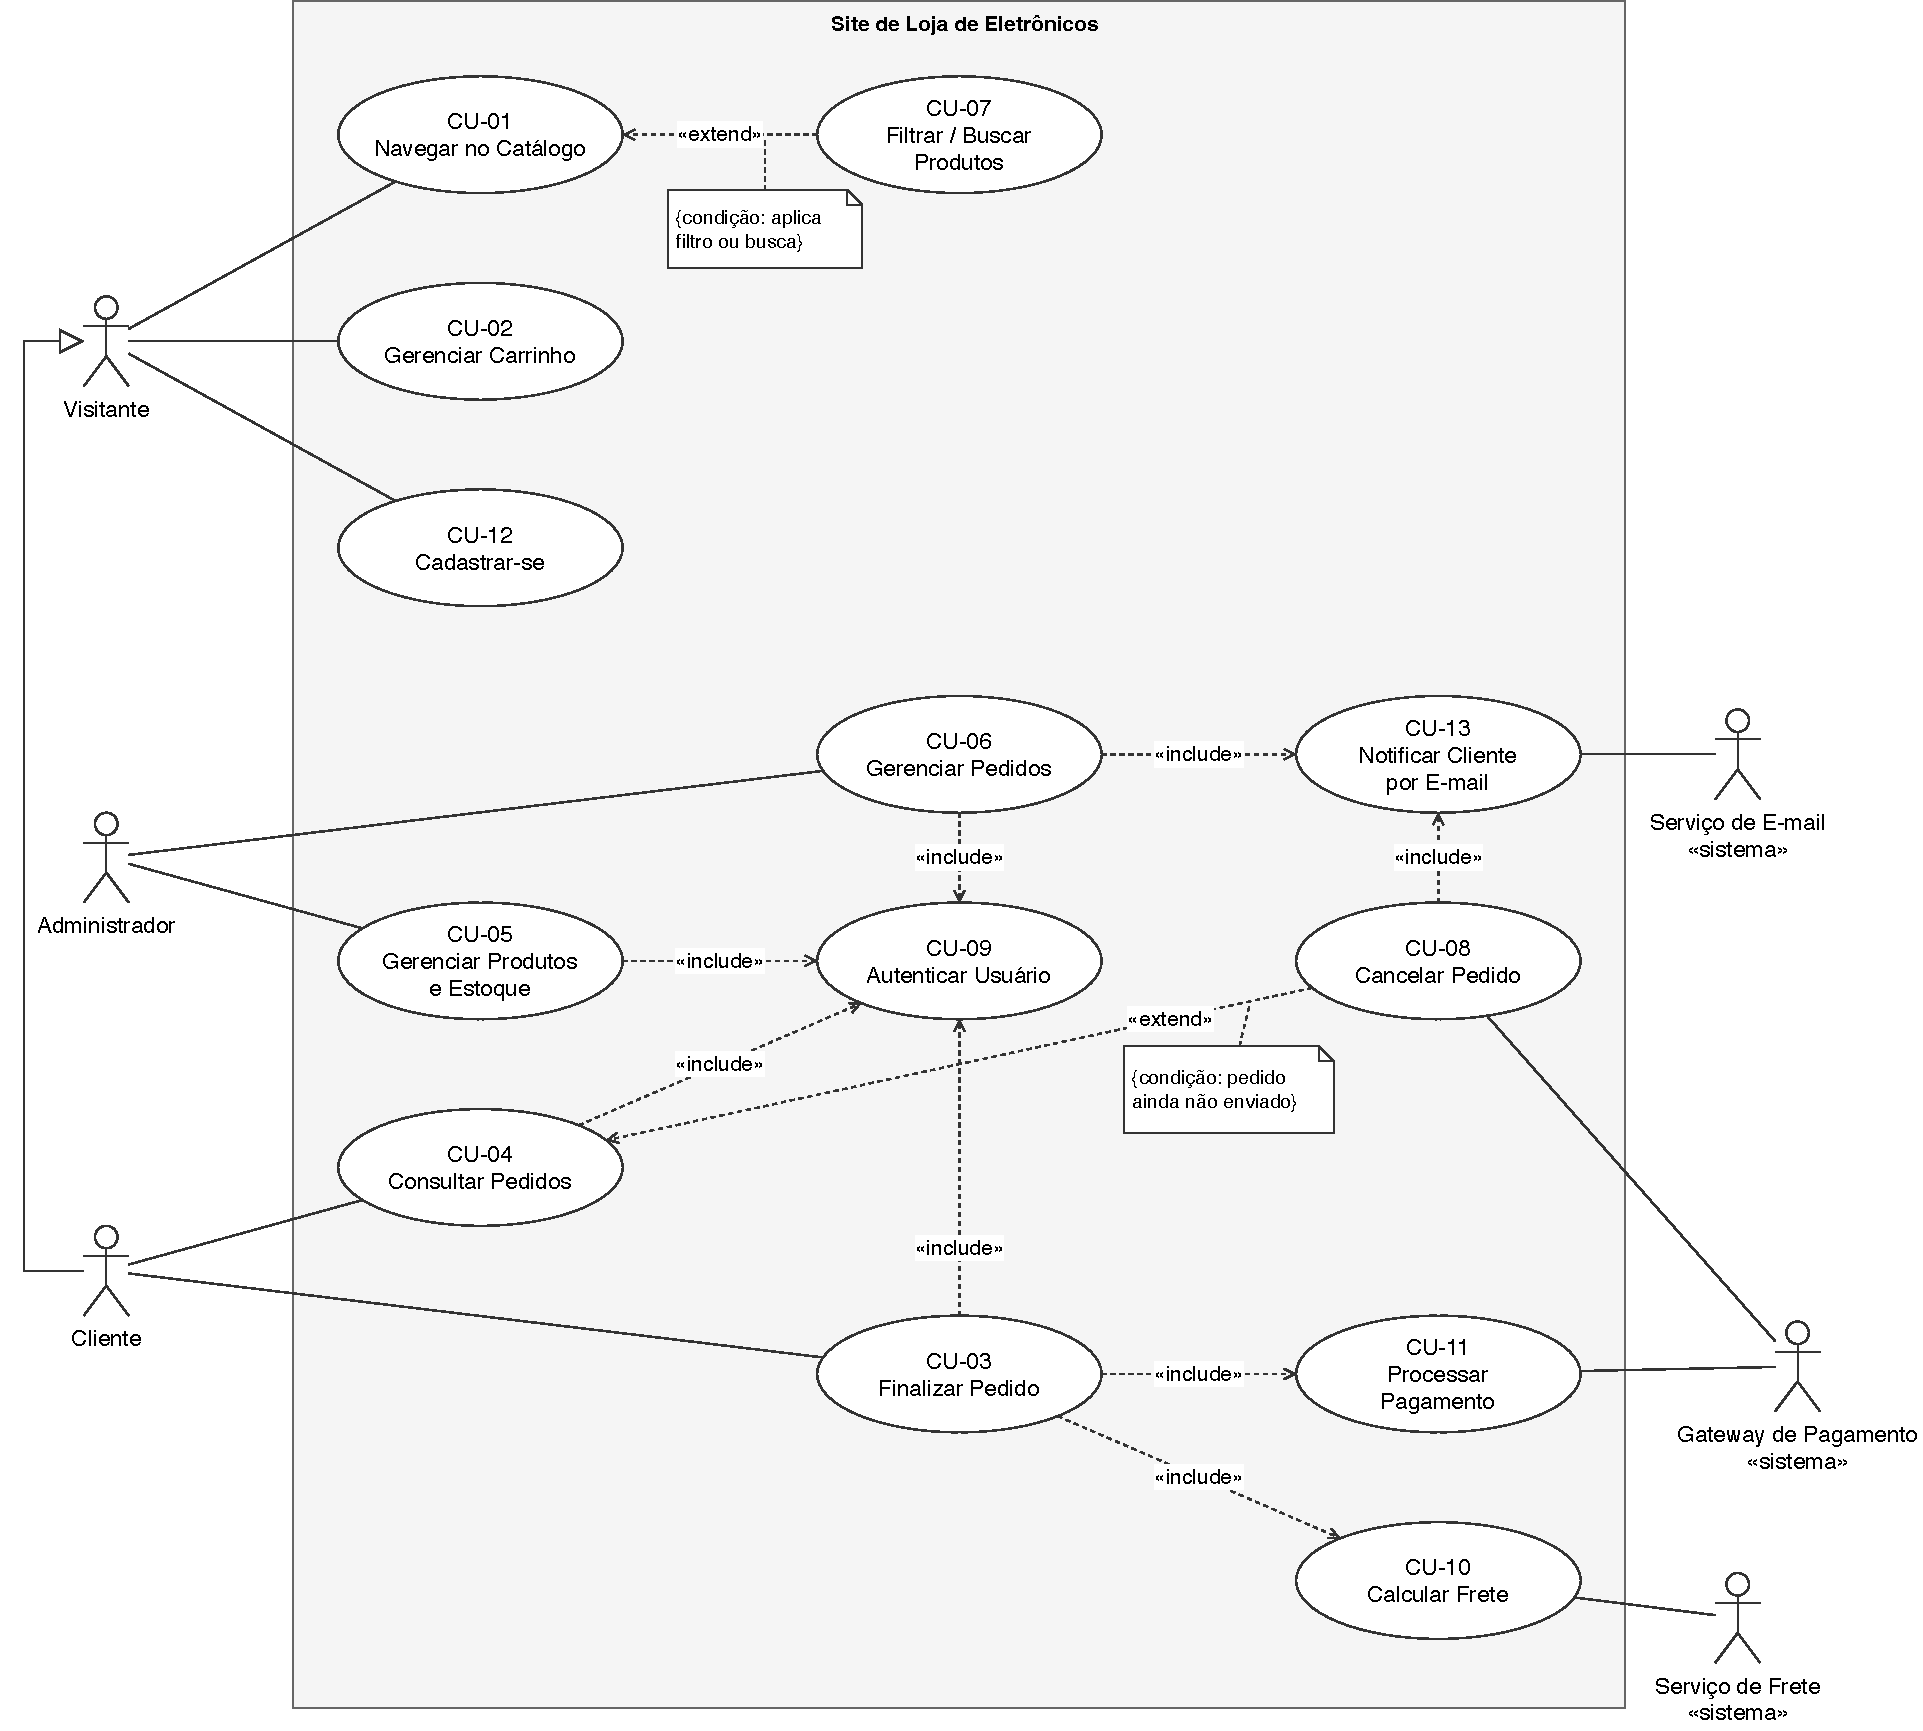
\includegraphics[trim=140.0bp 217.9bp 142.7bp 14.2bp, clip, width=185.0pt]{CU_CasosDeUso.pdf}};
  \hl{96.3}{69.3}{138.7}{88.4}{Destaque}
  \hl{162.8}{183.9}{205.1}{203.0}{Destaque}
  \hl{29.9}{69.3}{72.2}{88.4}{Navy}
  \hl{29.9}{212.6}{72.2}{231.7}{Navy}
  \pcu{218.0}{64.0}{211.0}{80.5}{Apoio}{CU-07 Filtrar / Buscar}
    {\textbf{Ator:} Visitante. \textbf{Pré:} lista do CU-01.}
    {1. Escolhe filtros ou digita um termo.\par 2. Sistema aplica os filtros.\par 3. Lista atualizada.}
    {\textbf{A1} Sem resultado: limpar.\par \textbf{E1} Faixa de preço inválida.}
  \pcu{218.0}{148.5}{211.0}{88.5}{Apoio}{CU-08 Cancelar Pedido}
    {\textbf{Atores:} Cliente e Gateway. \textbf{Pré:} pedido ainda não enviado.}
    {1. Pede o cancelamento e o motivo.\par 2. Confirma.\par 3. Sistema cancela e devolve o estoque.\par 4. Avisa o cliente (CU-13).}
    {\textbf{A1 · A2} Já pago: estorno; desiste.\par \textbf{E1 · E2} Já enviado; estorno pendente.}
\end{tela}\end{frame}

% --- Kayque ---
\begin{frame}[plain]\begin{tela}
  \fundo{2.4}{ESPECIFICAÇÃO · CU-09 · CU-10}{Autenticar e calcular o frete}
    {O login reutilizado e o primeiro caso com sistema externo (Tabelas 12 e 13)}
  \fill[white] \pto{25}{64} rectangle \pto{210}{237};
  \draw[Borda, line width=0.5pt] \pto{25}{64} rectangle \pto{210}{237};
  \node[anchor=north west, inner sep=0pt] at \pto{25.0}{64.0} {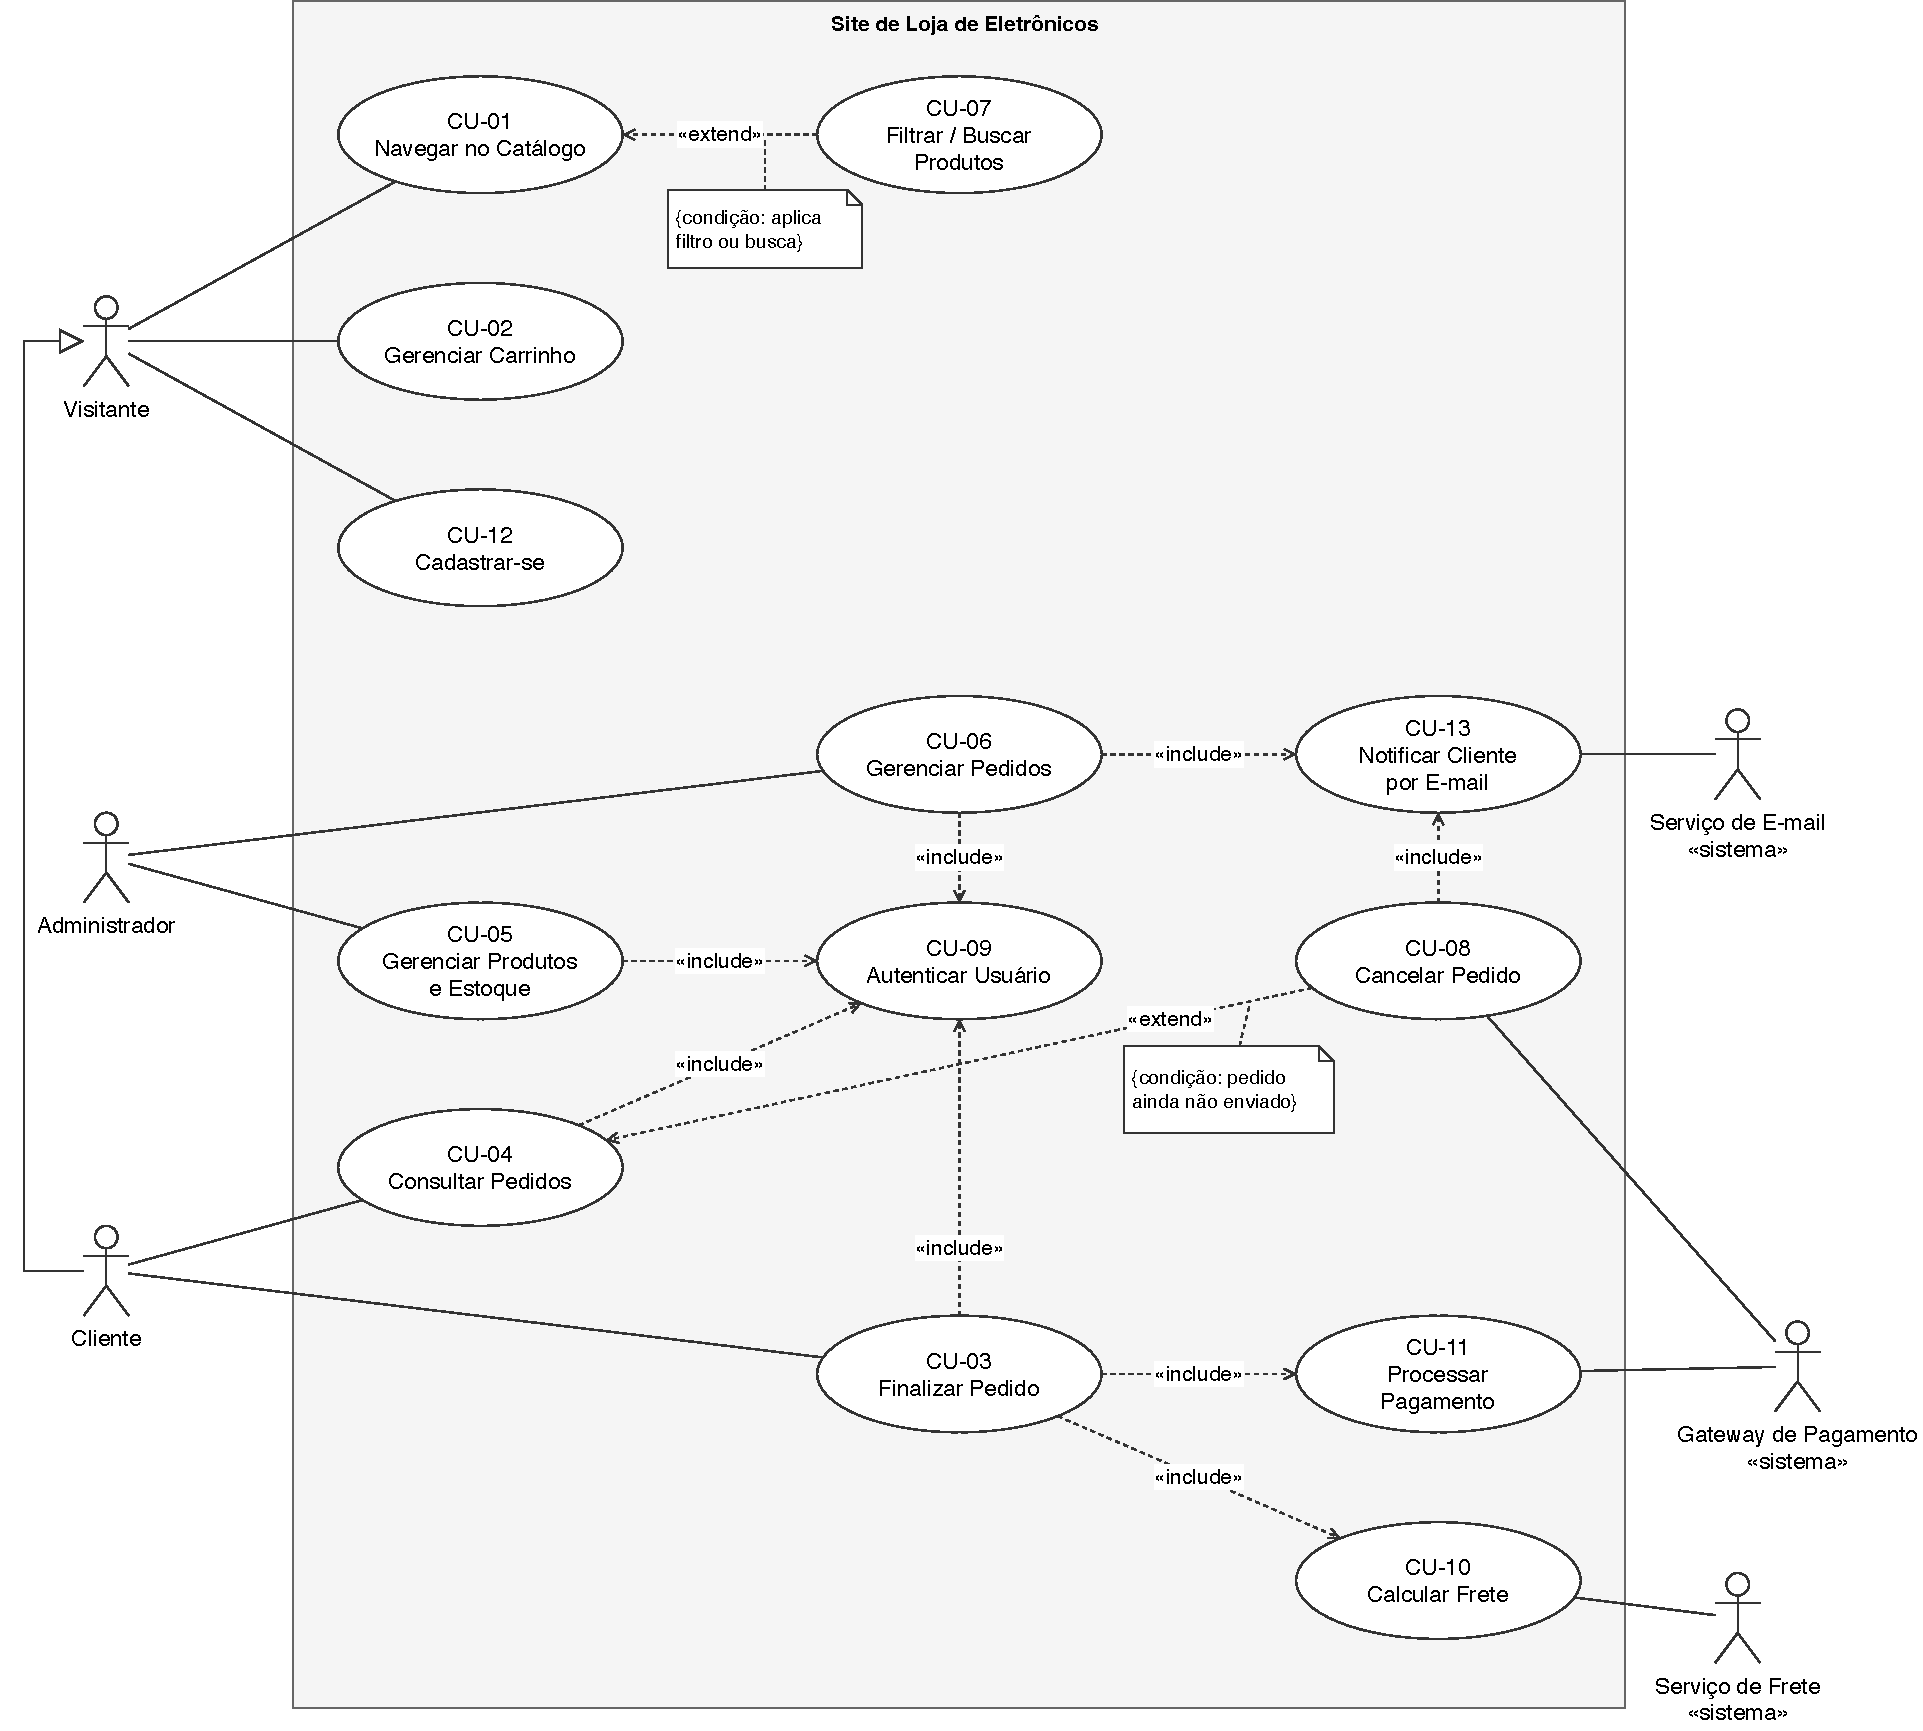
\includegraphics[trim=369.9bp 0.0bp 56.5bp 366.5bp, clip, width=185.0pt]{CU_CasosDeUso.pdf}};
  \hl{31.3}{87.4}{85.9}{112.0}{Destaque}
  \hl{117.0}{198.2}{171.6}{222.8}{Destaque}
  \hl{31.3}{161.2}{85.9}{185.9}{Navy}
  \pcu{218.0}{64.0}{211.0}{88.5}{Apoio}{CU-09 Autenticar Usuário}
    {\textbf{Atores:} Cliente e Administrador. \textbf{Pré:} conta cadastrada.}
    {1. Informa e-mail e senha.\par 2. Sistema valida.\par 3. Identifica o perfil e abre a sessão.\par 4. Volta ao ponto anterior.}
    {\textbf{A1} Sem conta: CU-12.\par \textbf{E1} Inválido: mensagem genérica.}
  \pcu{218.0}{156.5}{211.0}{80.5}{Apoio}{CU-10 Calcular Frete}
    {\textbf{Ator:} Serviço de Frete. \textbf{Pré:} CEP informado.}
    {1. Envia CEP, peso e medidas.\par 2. Serviço devolve as opções.\par 3. Exibe valor e prazo (CU-03).}
    {\textbf{E1} CEP inválido.\par \textbf{E2} Serviço fora do ar: não avança.}
\end{tela}\end{frame}

% --- Kayque ---
\begin{frame}[plain]\begin{tela}
  \fundo{2.4}{ESPECIFICAÇÃO · CU-11}{CU-11: o pagamento passa pelo gateway}
    {Cobrança, confirmação e prazo de Pix e boleto (Tabela 14)}
  \fill[white] \pto{25}{64} rectangle \pto{260}{237};
  \draw[Borda, line width=0.5pt] \pto{25}{64} rectangle \pto{260}{237};
  \node[anchor=north west, inner sep=0pt] at \pto{25.0}{64.0} {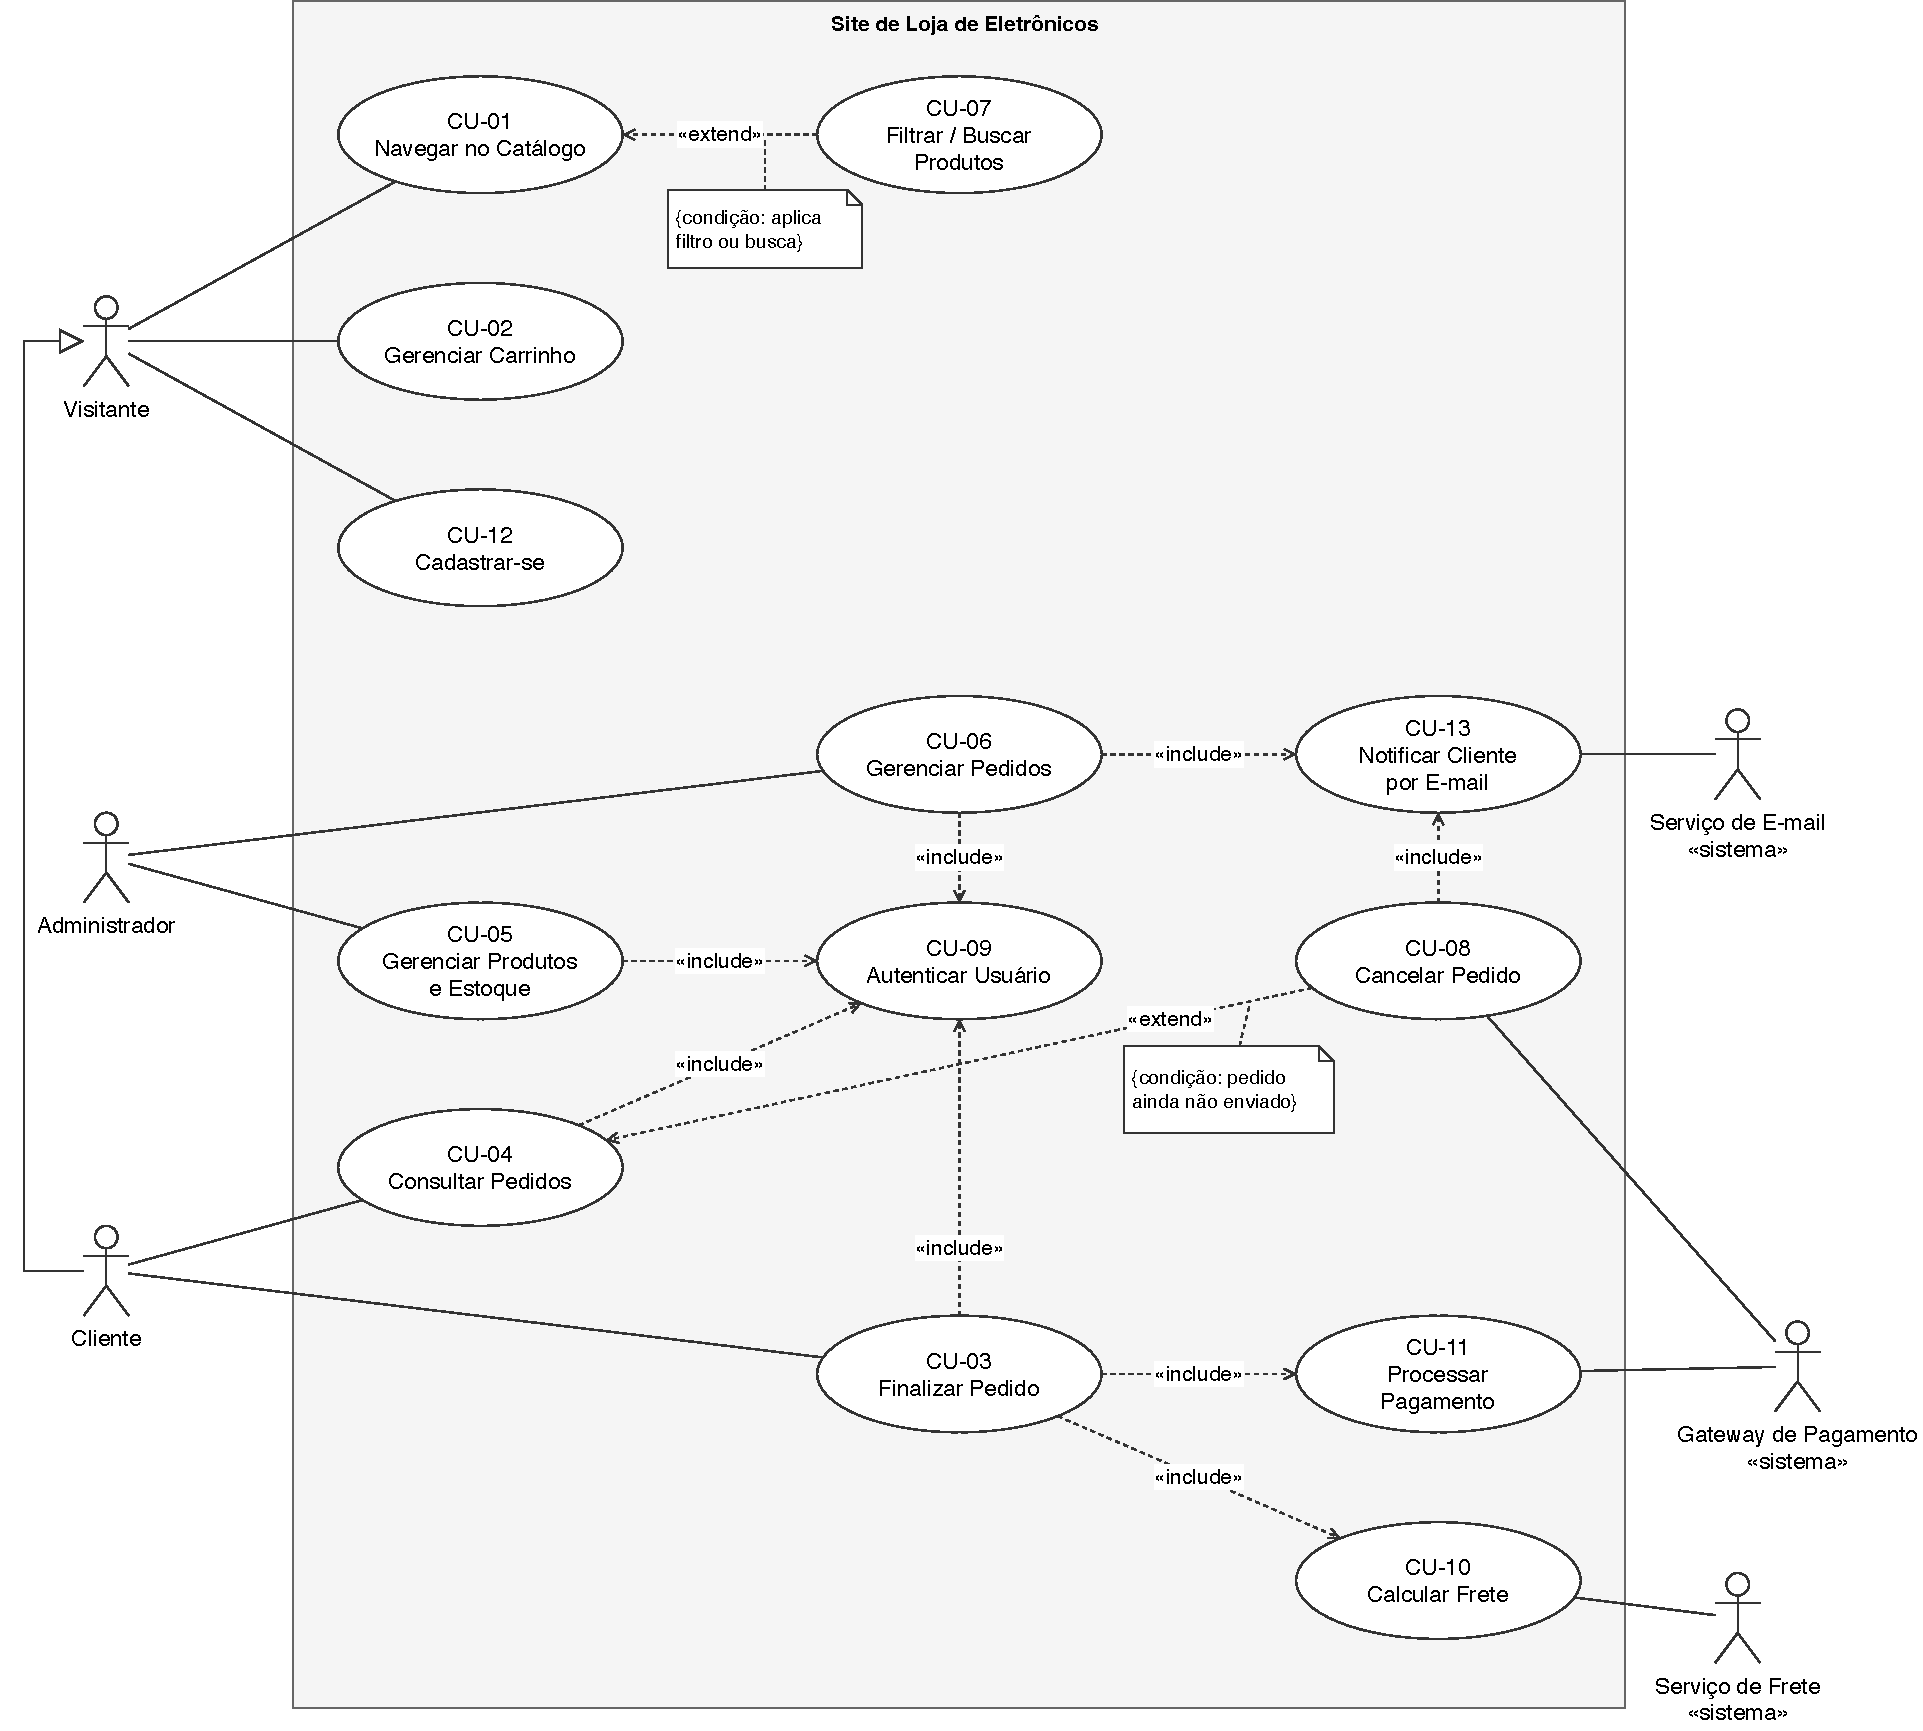
\includegraphics[trim=369.9bp 76.1bp 27.8bp 368.0bp, clip, width=235.0pt]{CU_CasosDeUso.pdf}};
  \hl{135.4}{180.1}{201.0}{209.6}{Destaque}
  \hl{32.6}{180.1}{98.1}{209.6}{Navy}
  \pcu{268.0}{64.0}{161.0}{173.0}{Apoio}{CU-11 Processar Pagamento}
    {\textbf{Ator:} Gateway de Pagamento. \textbf{Pré:} pedido criado.}
    {1. Envia a cobrança, sem guardar cartão.\par 2. Gateway aprova.\par 3. Sistema registra o resultado.\par 4. Pedido pago; estoque baixado.}
    {\textbf{A1} Pix ou boleto aguardam.\par \textbf{E1} Recusado: volta ao CU-03.\par \textbf{E2} Gateway fora: verificação.\par \textbf{E3} Prazo expira: cancela.}
\end{tela}\end{frame}

% --- Kayque ---
\begin{frame}[plain]\begin{tela}
  \fundo{2.4}{ESPECIFICAÇÃO · CU-12 · CU-13}{Cadastrar-se e avisar o cliente}
    {Como o Visitante vira Cliente, e como o cliente fica sabendo do pedido (Tabelas 15 e 16)}
  \fill[white] \pto{25}{64} rectangle \pto{210}{237};
  \draw[Borda, line width=0.5pt] \pto{25}{64} rectangle \pto{210}{237};
  \node[anchor=north west, inner sep=0pt] at \pto{25.0}{67.2} {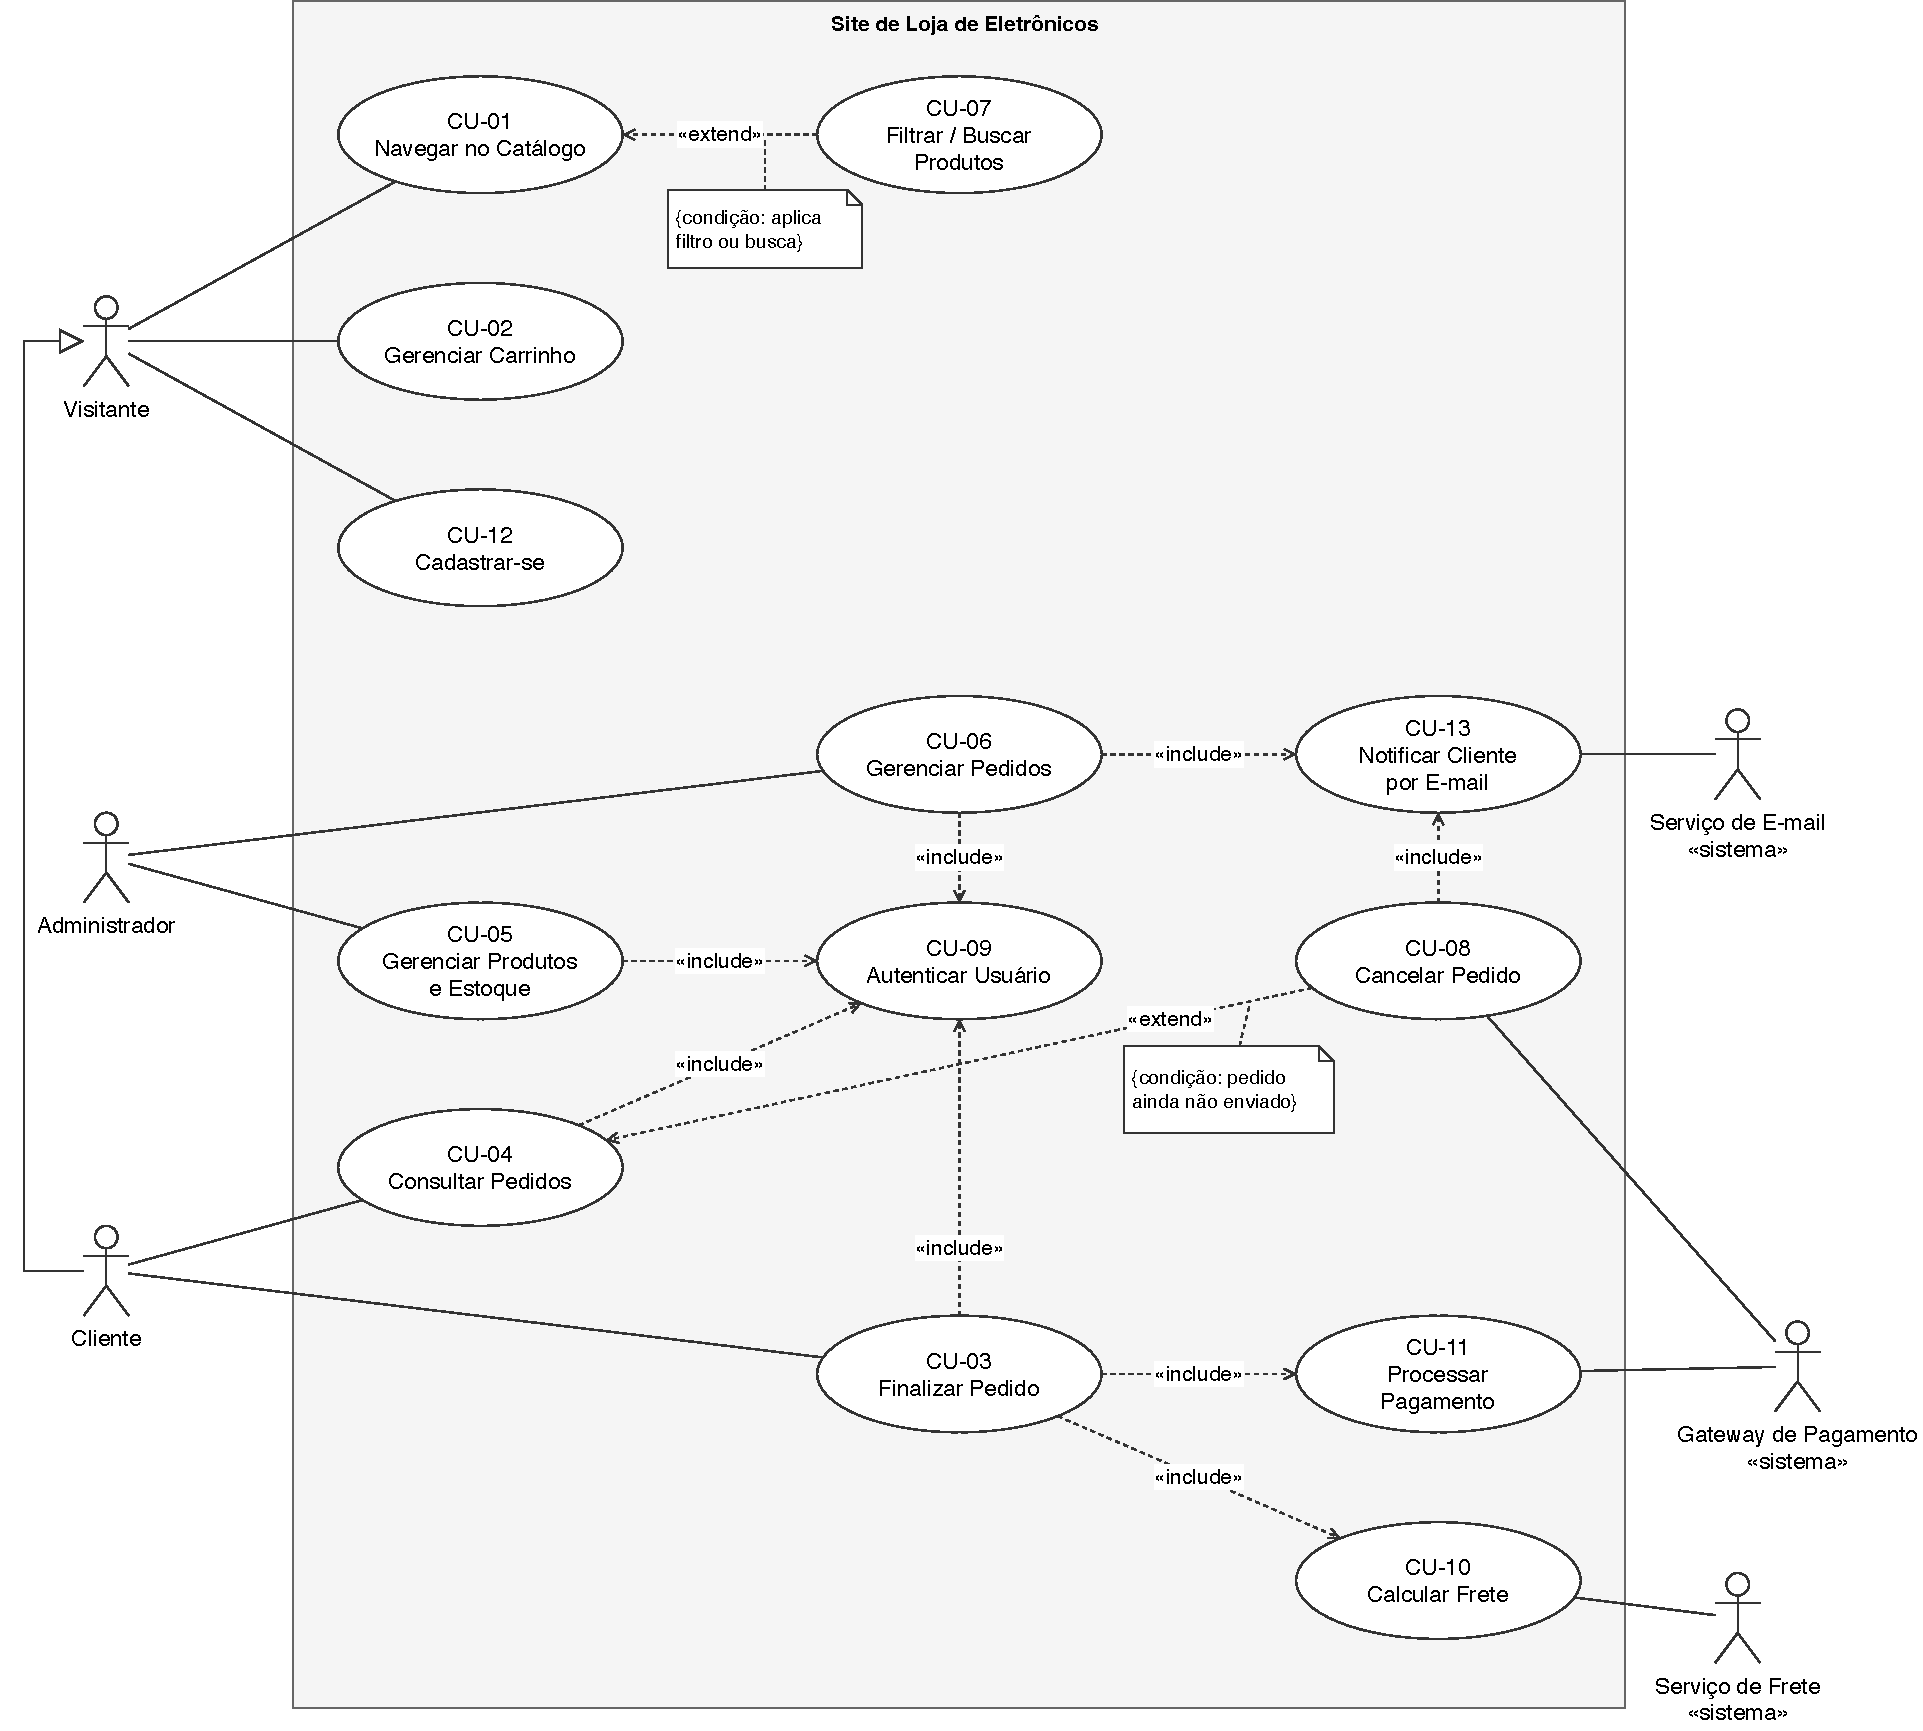
\includegraphics[trim=0.0bp 0.0bp 0.0bp 0.0bp, clip, width=185.0pt]{CU_CasosDeUso.pdf}};
  \hl{56.5}{113.5}{85.8}{126.8}{Destaque}
  \hl{148.6}{133.4}{178.0}{146.6}{Destaque}
  \hl{32.0}{95.0}{38.3}{105.6}{Navy}
  \hl{188.9}{134.7}{195.3}{145.3}{Navy}
  \pcu{218.0}{64.0}{211.0}{84.5}{Principal}{CU-12 Cadastrar-se}
    {\textbf{Ator:} Visitante. \textbf{Pré:} nenhuma.}
    {1. Informa dados e senha.\par 2. Sistema valida.\par 3. Cria a conta e autentica.}
    {\textbf{E1} CPF ou e-mail já usado.\par \textbf{E2} Dados inválidos.}
  \pcu{218.0}{152.5}{211.0}{84.5}{Apoio}{CU-13 Notificar Cliente por E-mail}
    {\textbf{Ator:} Serviço de E-mail. \textbf{Pré:} status alterado.}
    {1. Monta a mensagem.\par 2. Envia ao serviço.\par 3. Serviço entrega.\par 4. Registra o envio.}
    {\textbf{E1} Falha: tenta de novo, sem desfazer.}
\end{tela}\end{frame}

% =============================================================================
\section{Diagramas de Componentes}
% =============================================================================

% --- Luiz ---
\begin{frame}[plain]\begin{tela}
  \fundo{3}{COMPONENTES}{Uma aplicação web em cinco pacotes}
    {Diagrama geral (Figura 2) e dois detalhes internos: Frontend e Backend}
  \fill[white] \pto{25}{64} rectangle \pto{325}{237};
  \draw[Borda, line width=0.5pt] \pto{25}{64} rectangle \pto{325}{237};
  \node[anchor=north west, inner sep=0pt] at \pto{25.0}{77.0} {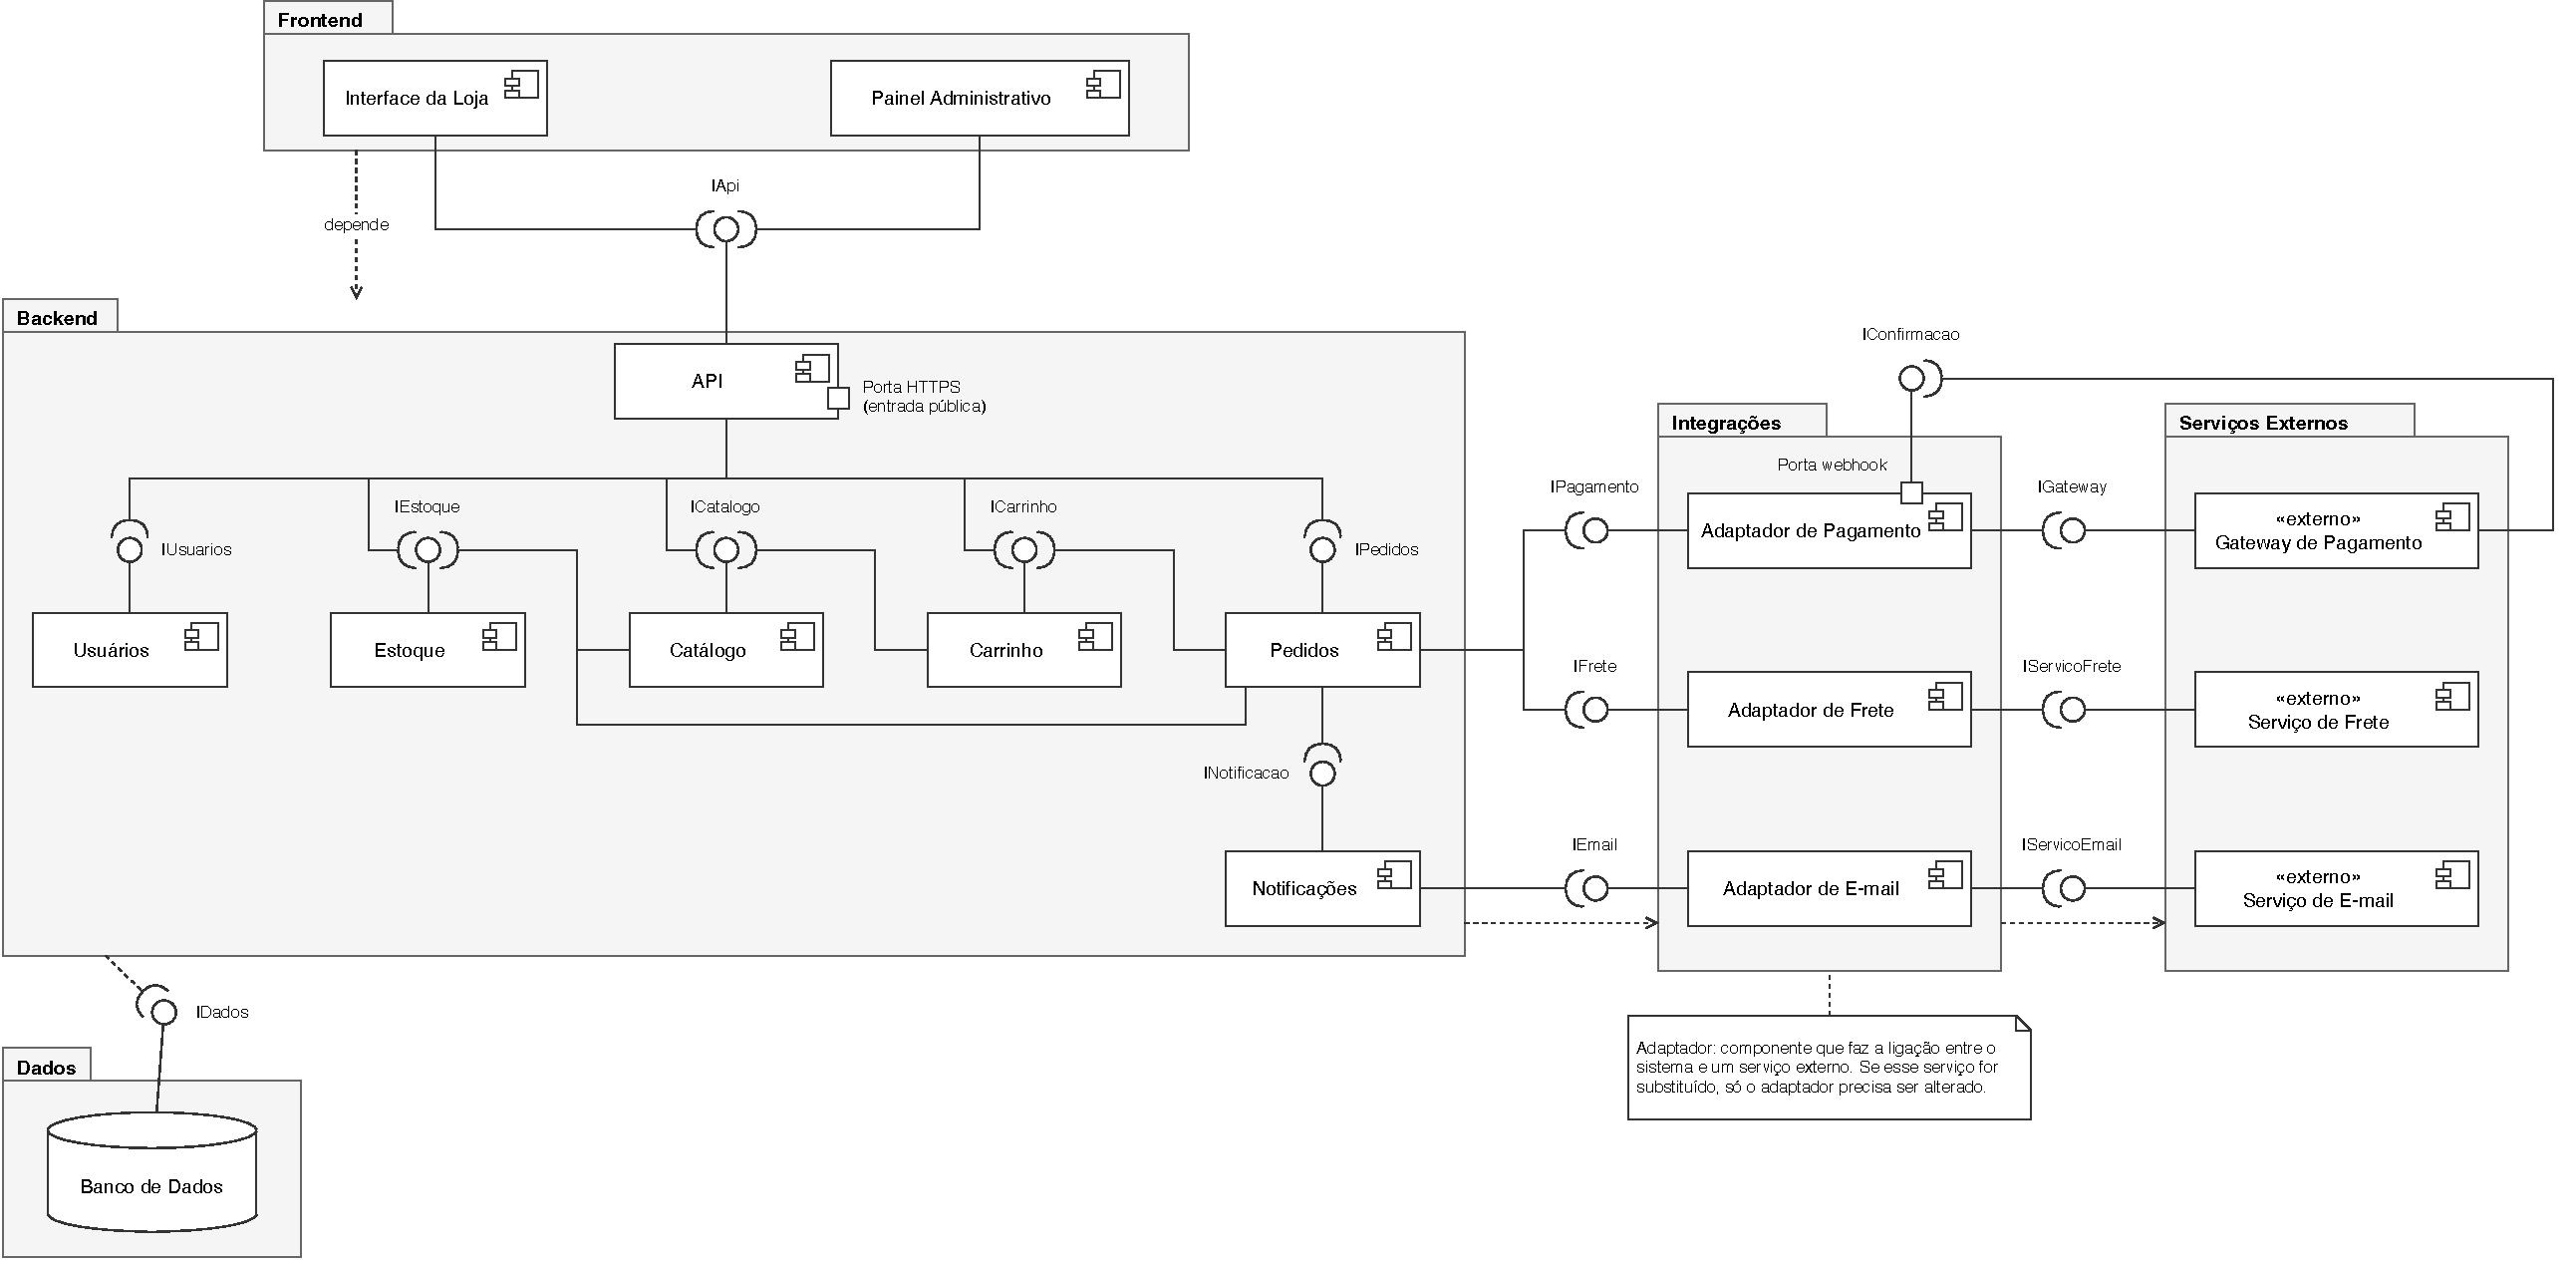
\includegraphics[trim=0.0bp 0.0bp 0.0bp 0.0bp, clip, width=300.0pt]{CMP_Geral.pdf}};
  \rot{107.4}{77.4}{PFront}{white}{Frontend}
  \rot{108.3}{110.4}{PBack}{white}{Backend}
  \rot{235.9}{124.2}{PInt}{Texto}{Integrações}
  \rot{294.9}{124.2}{PExt}{white}{Serviços Externos}
  \rot{55.0}{199.3}{PDados}{white}{Dados}
  \pcard{333}{64.0}{96}{55.0}{Navy}{Camadas}{Frontend, Backend, Integrações, Dados e Serviços Externos.}
  \pcard{333}{123.0}{96}{55.0}{PInt}{Adaptadores}{Trocar de serviço externo muda só o adaptador.}
  \pcard{333}{182.0}{96}{55.0}{PBack}{Dois níveis}{Geral e o detalhe do Frontend e do Backend.}
\end{tela}\end{frame}

% --- Luiz ---
\begin{frame}[plain]\begin{tela}
  \fundo{3.1}{LEITURA DO DIAGRAMA}{Como ler o diagrama de componentes}
    {Cada símbolo tem um significado; as cores identificam os pacotes}
  \fill[white] \pto{25}{64} rectangle \pto{290}{237};
  \draw[Borda, line width=0.5pt] \pto{25}{64} rectangle \pto{290}{237};
  \node[anchor=north west, inner sep=0pt] at \pto{25.0}{64.0} {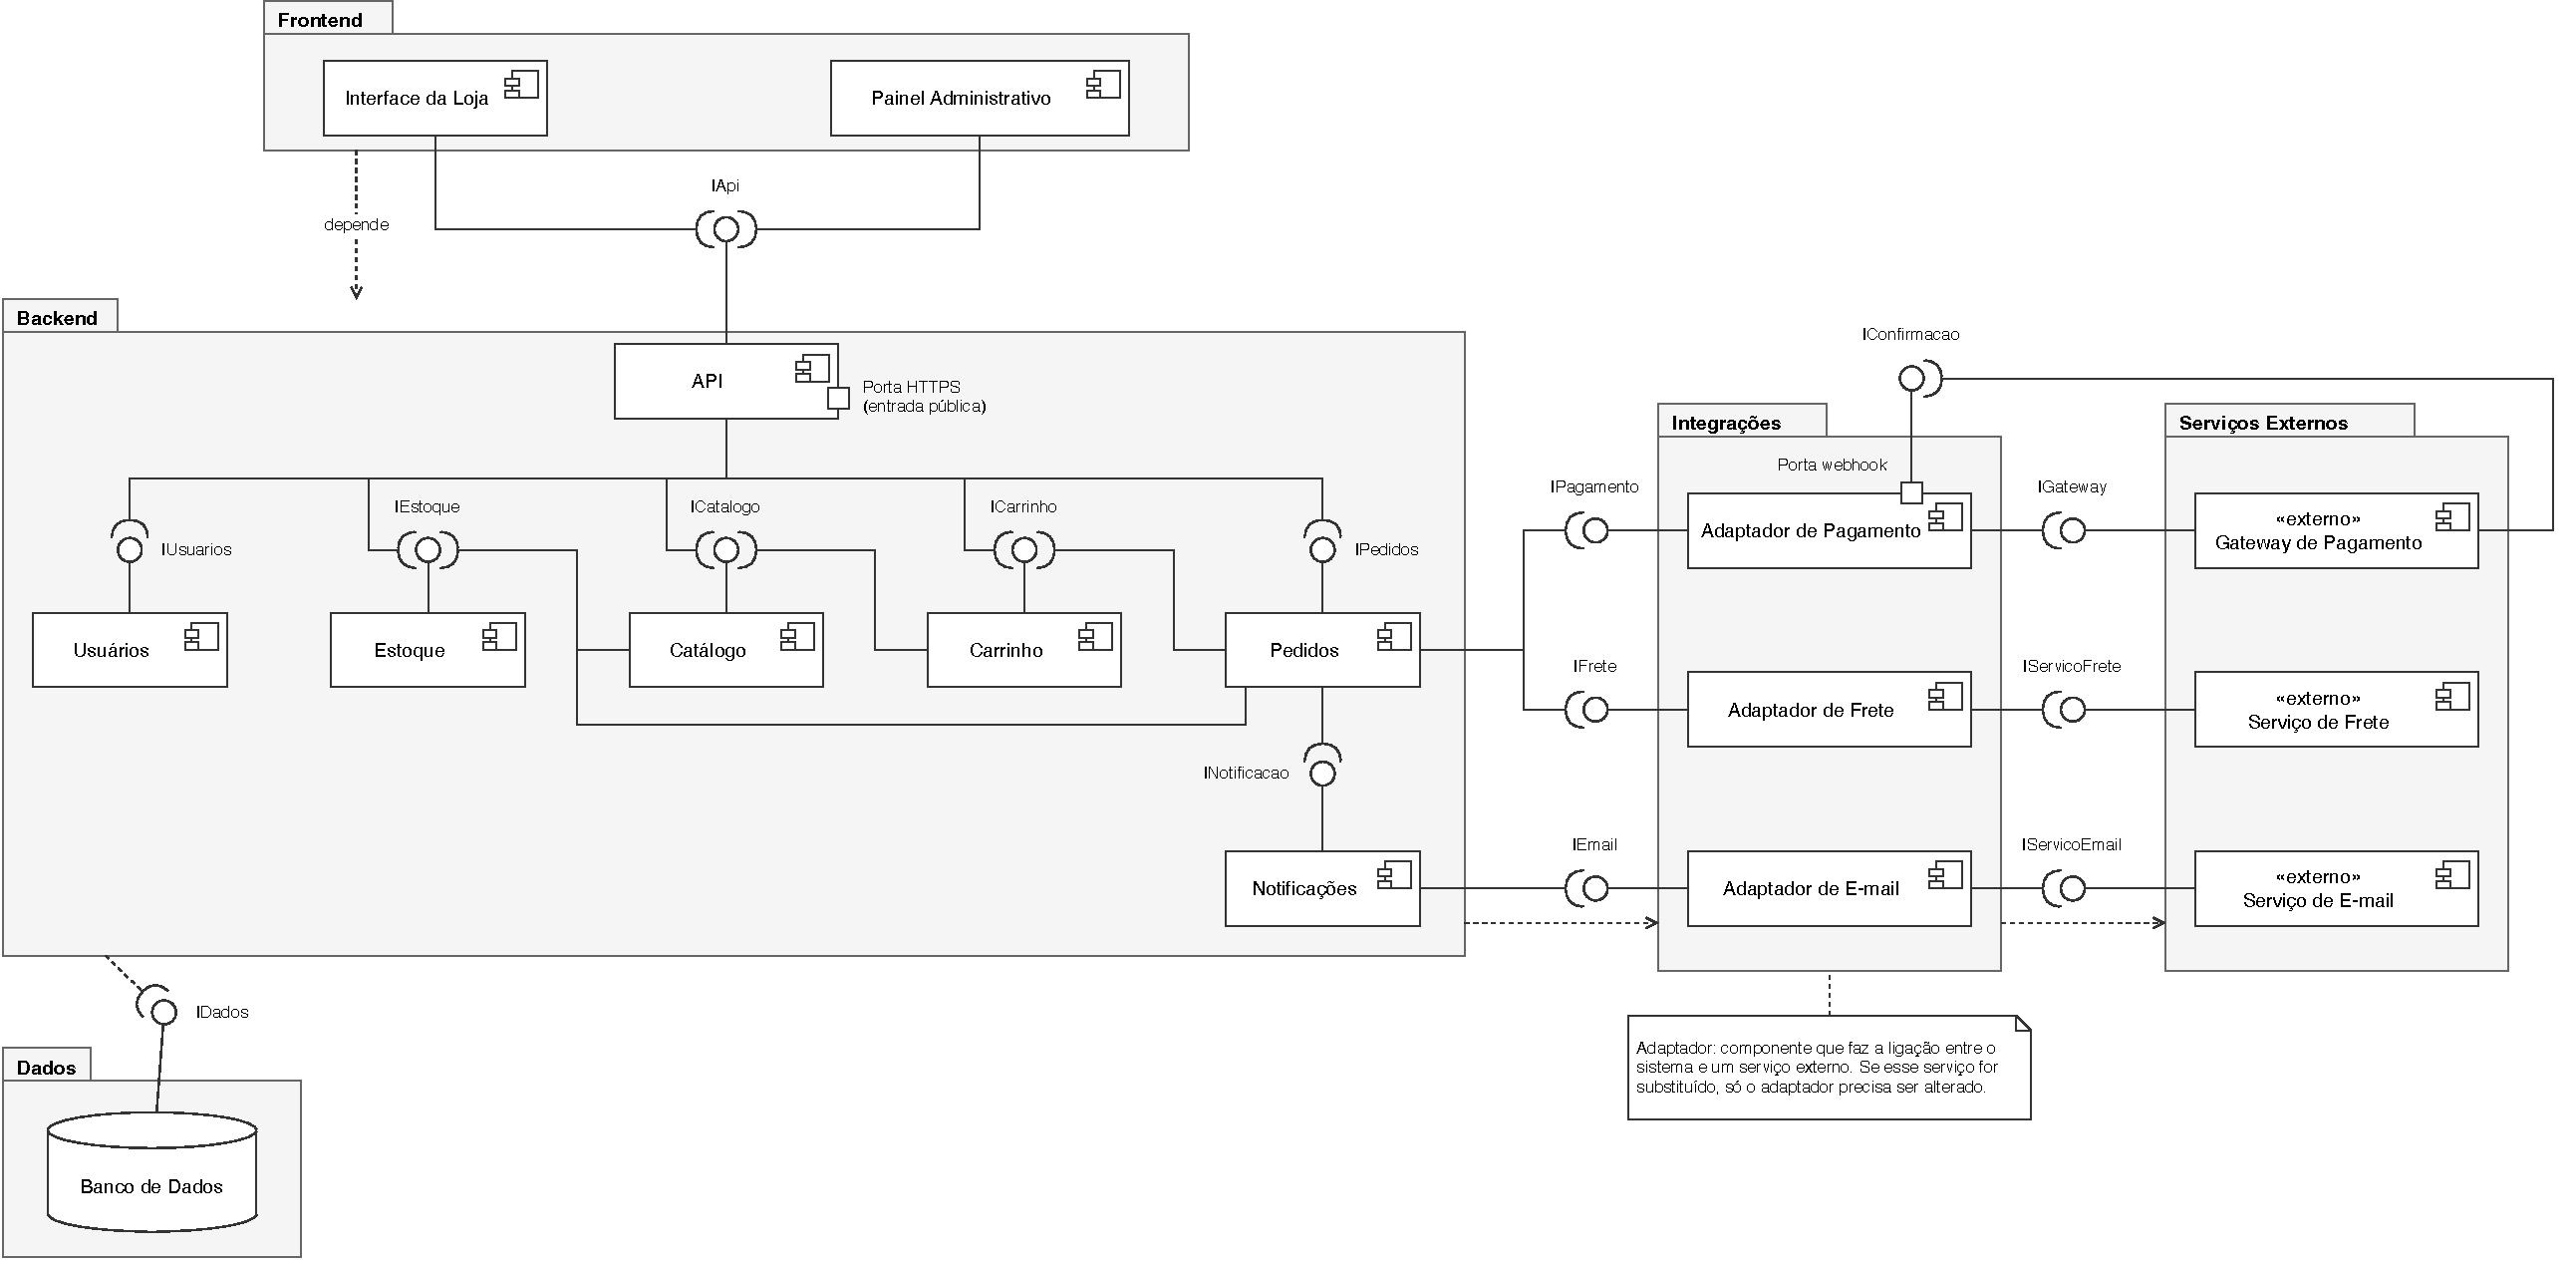
\includegraphics[trim=132.9bp 245.0bp 552.2bp 0.0bp, clip, width=265.0pt]{CMP_Geral.pdf}};
  \mk{96.5}{146.7}{1}
  \mk{128.8}{117.1}{2}
  \mk{57.4}{97.4}{3}
  \mk{166.1}{143.4}{4}
  \mk{32.0}{100.8}{5}
  \pnum{298}{64.0}{131}{31.4}{1}{\textbf{Componente:} retângulo com o ícone.}
  \pnum{298}{99.4}{131}{31.4}{2}{\textbf{Pirulito:} interface fornecida.}
  \pnum{298}{134.8}{131}{31.4}{3}{\textbf{Soquete:} interface requerida.}
  \pnum{298}{170.2}{131}{31.4}{4}{\textbf{Porta:} quadrado na borda.}
  \pnum{298}{205.6}{131}{31.4}{5}{\textbf{Seta tracejada:} dependência entre pacotes.}
\end{tela}\end{frame}

% --- Luiz ---
\begin{frame}[plain]\begin{tela}
  \fundo{3.1}{PERCURSO DE UM PEDIDO}{Finalizar Pedido atravessa todas as camadas}
    {O CU-03 visto pelo diagrama de componentes}
  \fill[white] \pto{25}{64} rectangle \pto{325}{237};
  \draw[Borda, line width=0.5pt] \pto{25}{64} rectangle \pto{325}{237};
  \node[anchor=north west, inner sep=0pt] at \pto{25.0}{77.0} {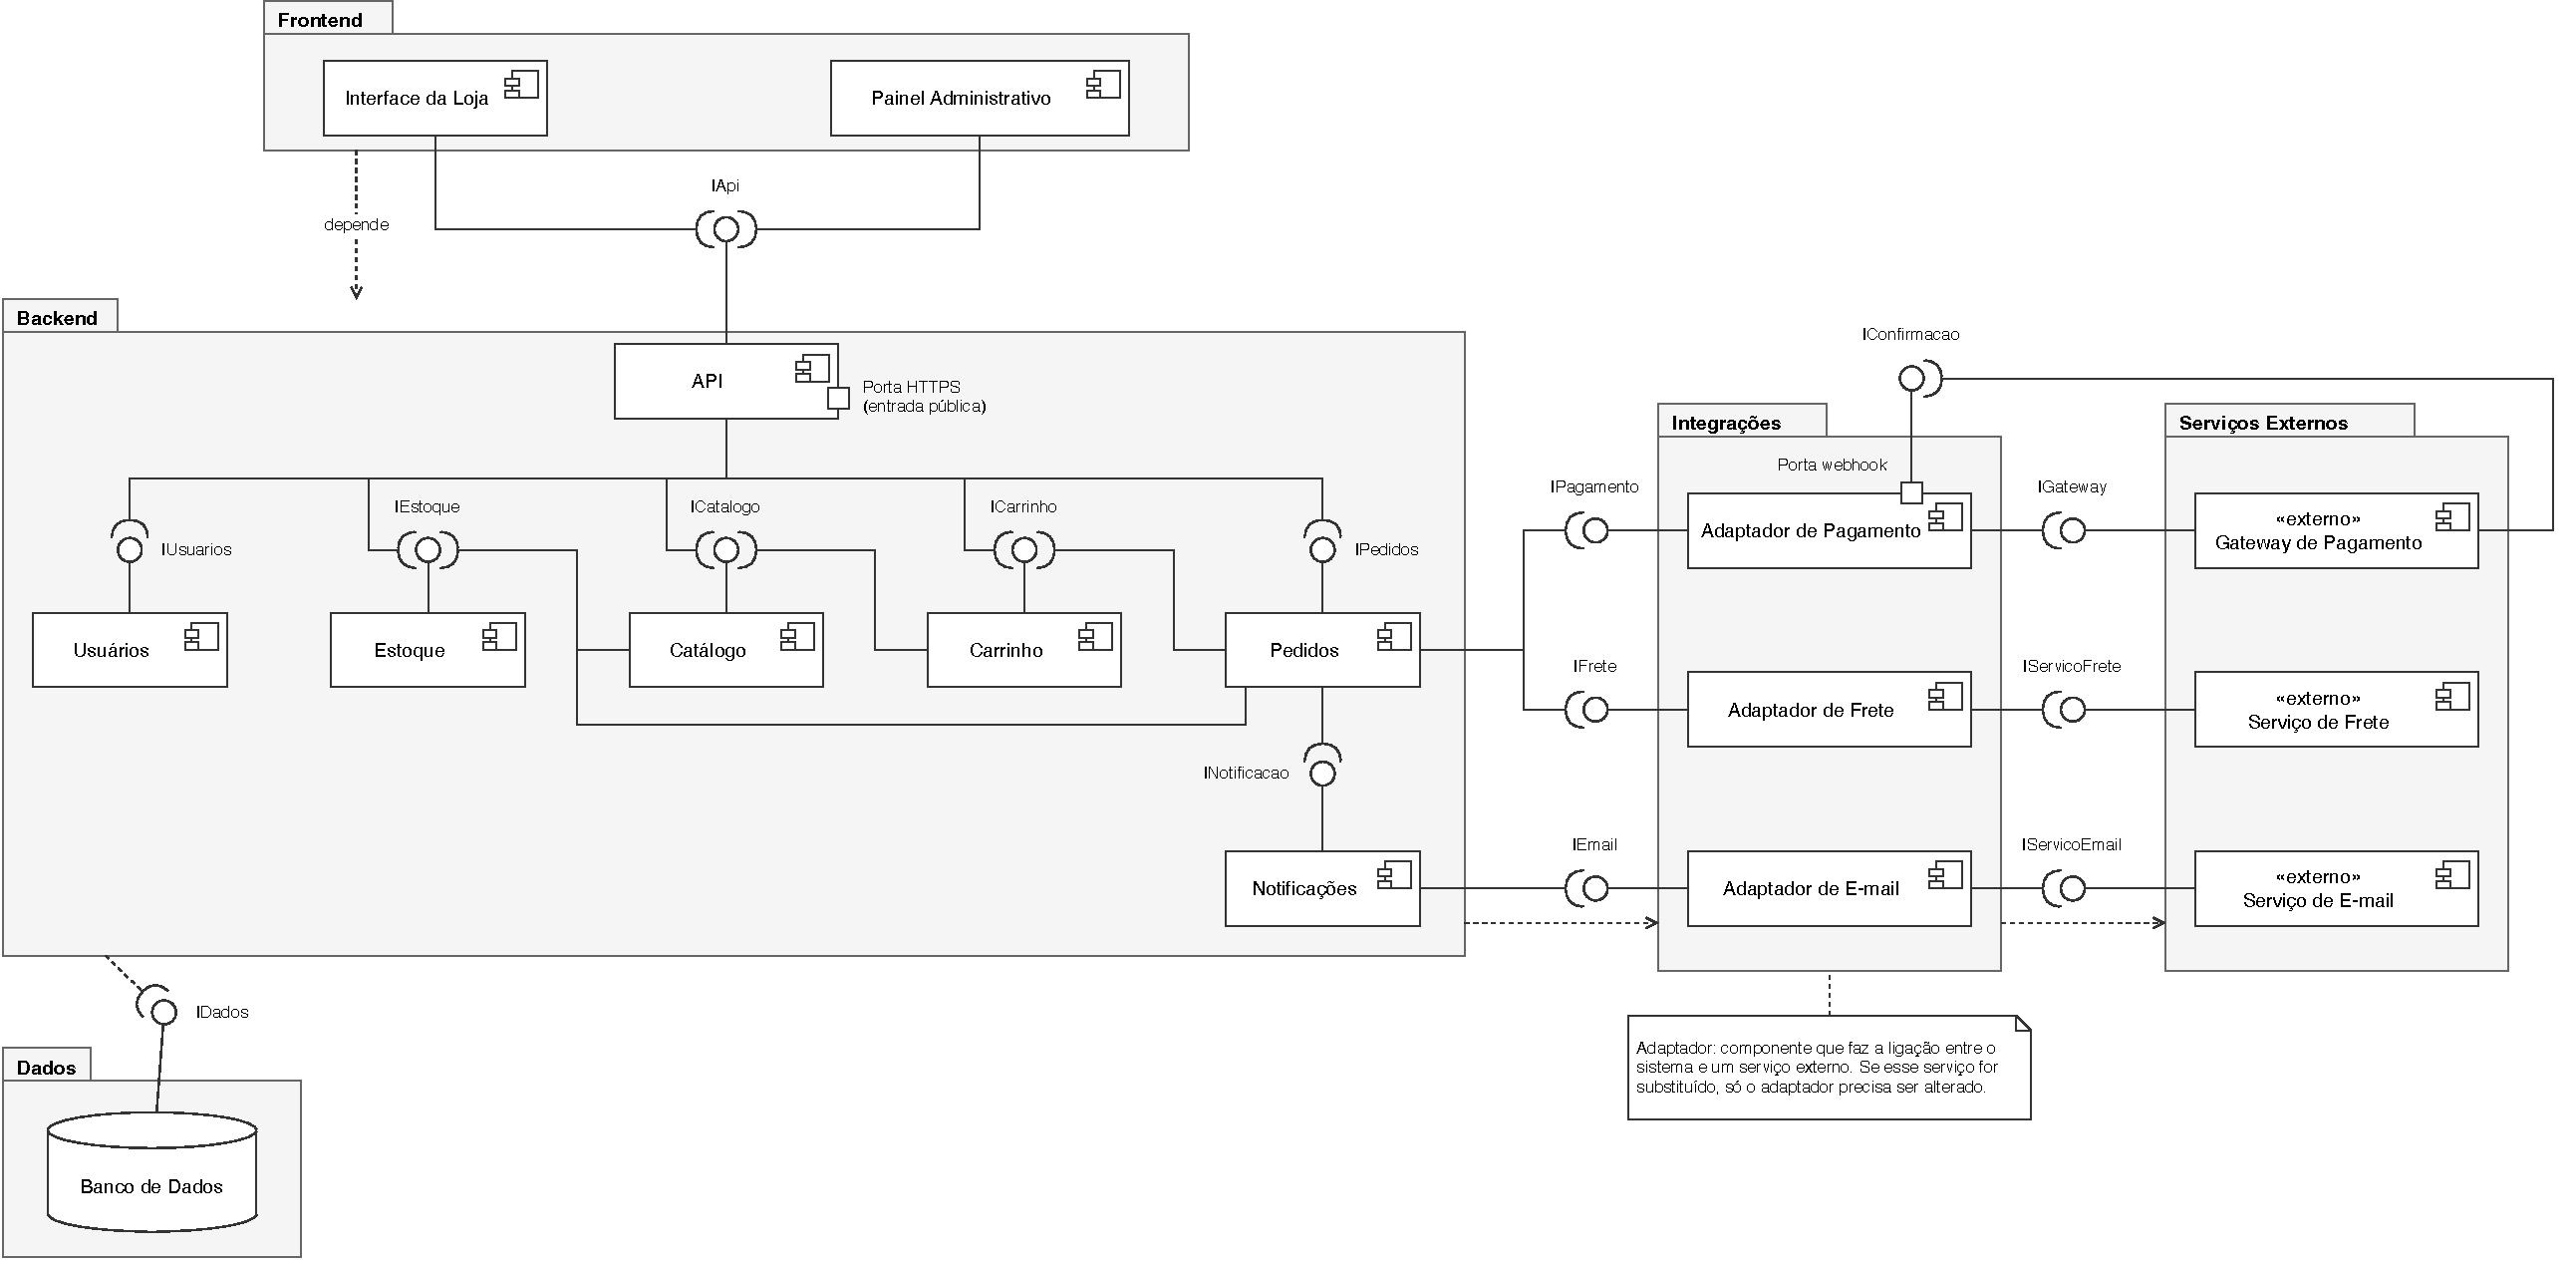
\includegraphics[trim=0.0bp 0.0bp 0.0bp 0.0bp, clip, width=300.0pt]{CMP_Geral.pdf}};
  \mk{87.5}{83.3}{1}
  \mk{189.1}{147.6}{2}
  \mk{218.4}{133.7}{3}
  \mk{243.1}{121.3}{4}
  \mk{189.1}{175.4}{5}
  \pnum{333}{64.0}{96}{31.4}{1}{Tela chama \texttt{IApi}.}
  \pnum{333}{99.4}{96}{31.4}{2}{Pedidos usa carrinho e estoque.}
  \pnum{333}{134.8}{96}{31.4}{3}{Adaptadores: frete e pagamento.}
  \pnum{333}{170.2}{96}{31.4}{4}{Webhook: \texttt{IConfirmacao} e \texttt{IPedidos}.}
  \pnum{333}{205.6}{96}{31.4}{5}{Aviso por e-mail; grava em \texttt{IDados}.}
\end{tela}\end{frame}

% --- Luiz ---
\begin{frame}[plain]\begin{tela}
  \fundo{3.2}{DECISÕES DE ARQUITETURA}{Seis decisões que dão forma à arquitetura}
    {Por que os componentes estão organizados assim (Seção 3.2)}
  \fill[white] \pto{25}{64} rectangle \pto{325}{237};
  \draw[Borda, line width=0.5pt] \pto{25}{64} rectangle \pto{325}{237};
  \node[anchor=north west, inner sep=0pt] at \pto{25.0}{77.0} {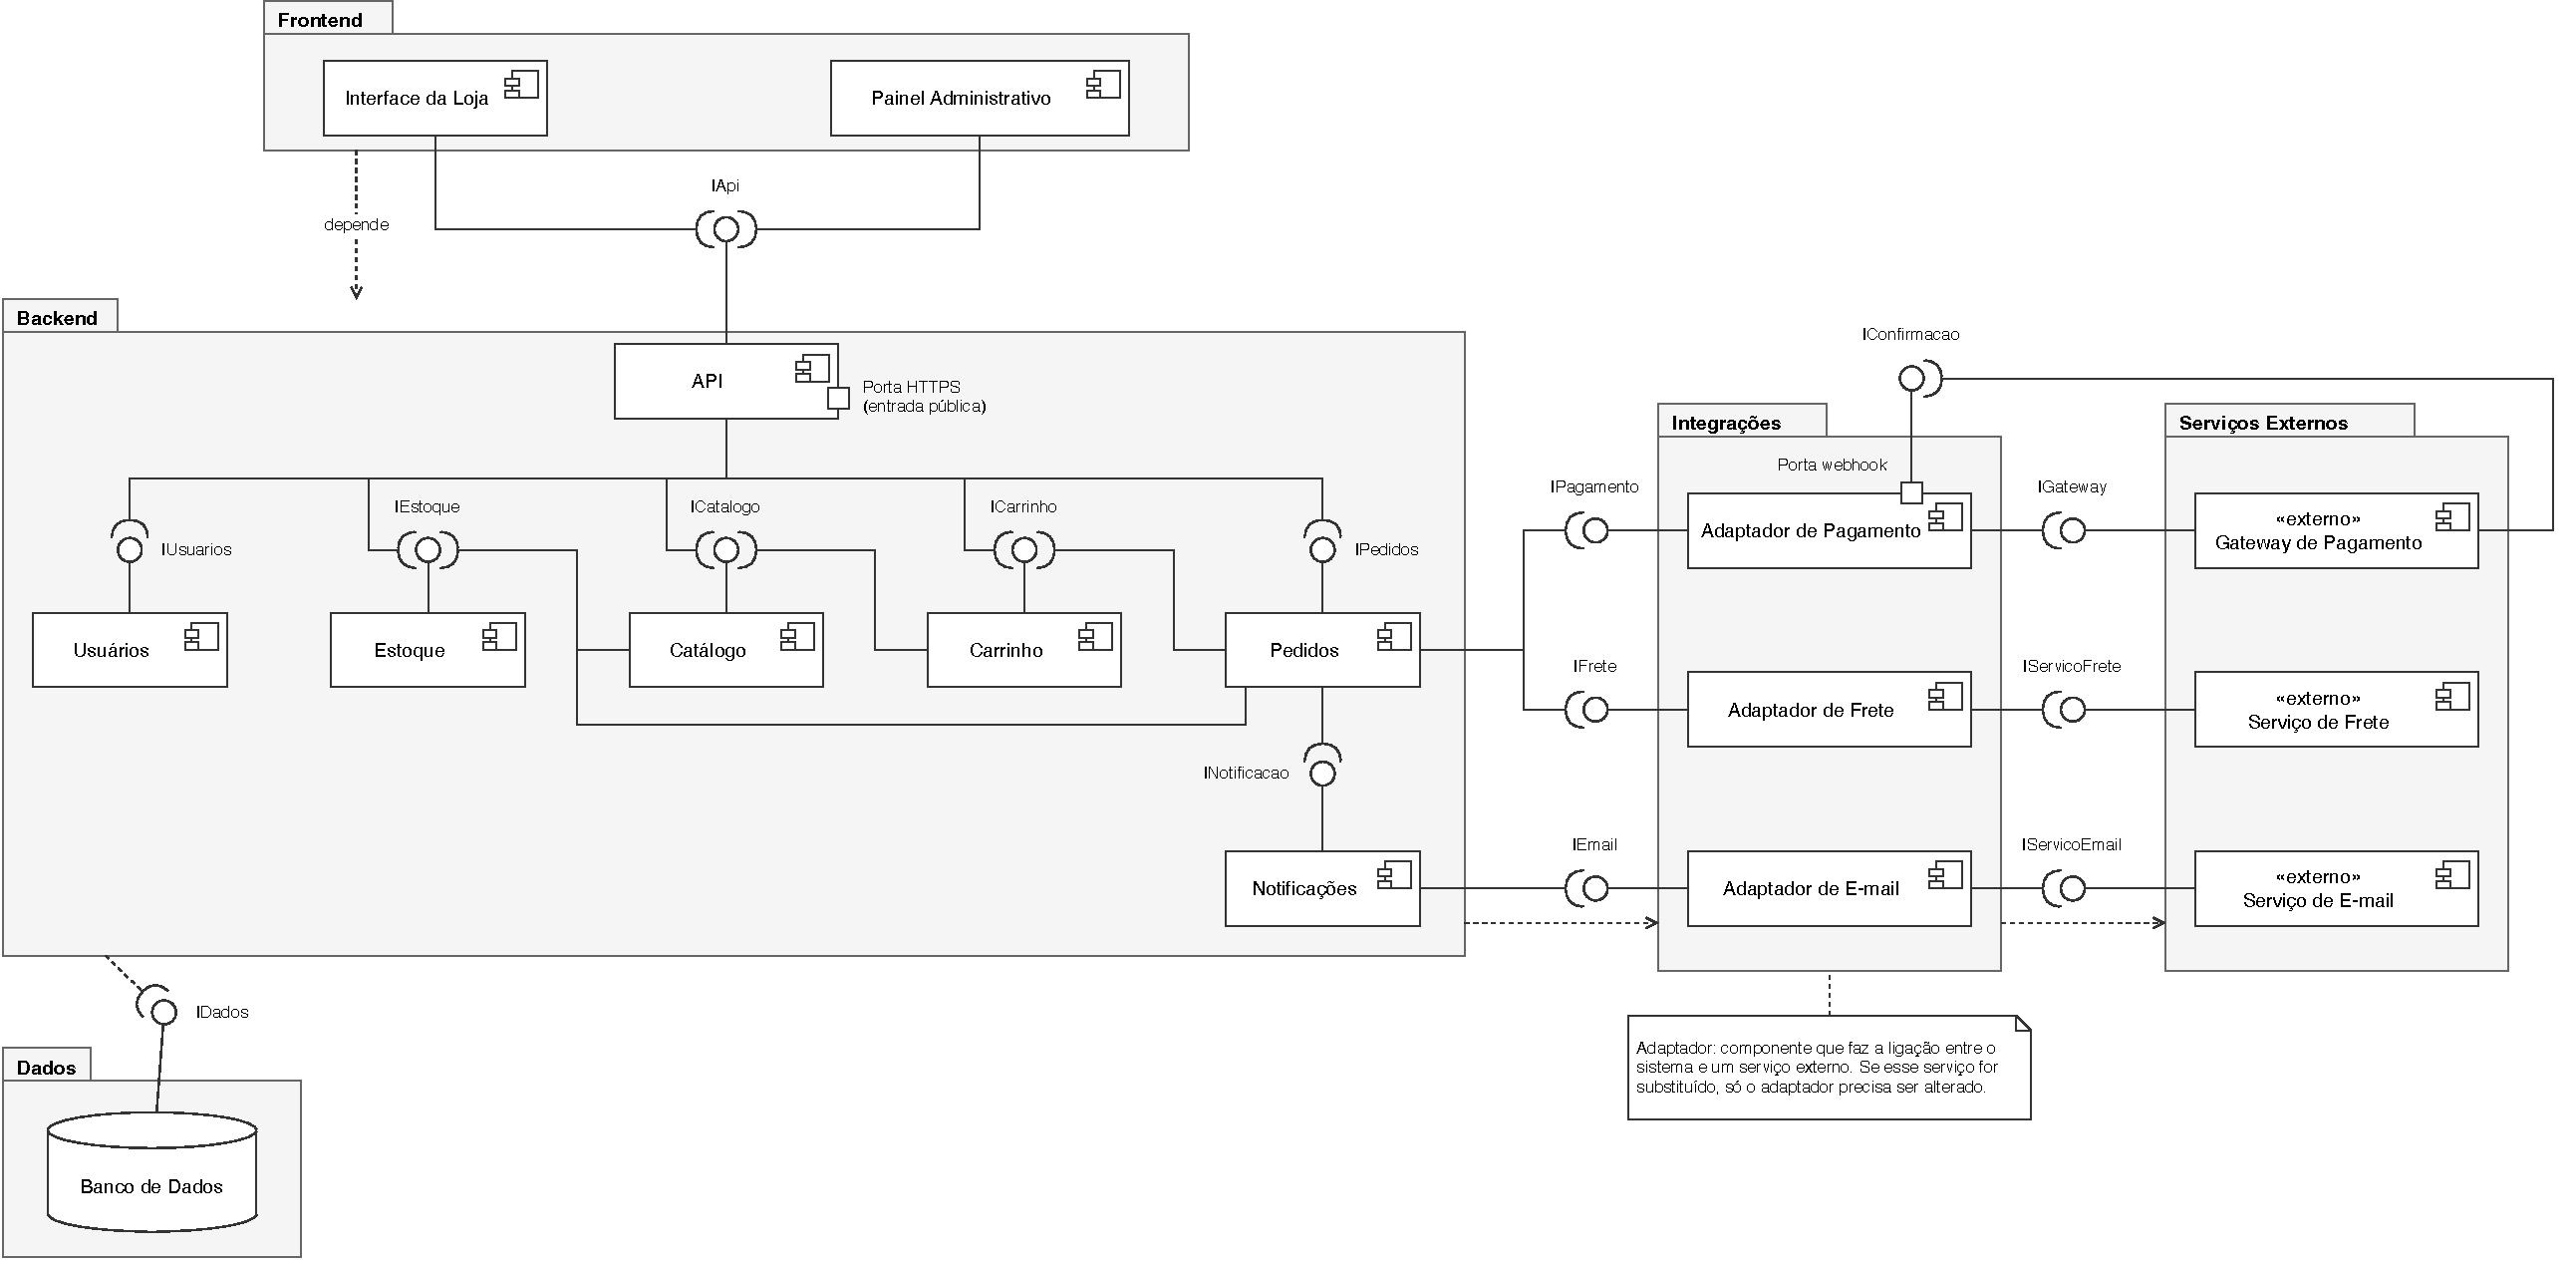
\includegraphics[trim=0.0bp 0.0bp 0.0bp 0.0bp, clip, width=300.0pt]{CMP_Geral.pdf}};
  \mk{32.0}{109.4}{1}
  \mk{121.4}{118.9}{2}
  \mk{215.0}{123.3}{3}
  \mk{243.1}{121.3}{4}
  \mk{53.7}{205.8}{5}
  \mk{52.6}{76.4}{6}
  \pnum{333}{64.0}{96}{25.5}{1}{Camadas, em um só sentido.}
  \pnum{333}{93.5}{96}{25.5}{2}{API é a única entrada.}
  \pnum{333}{123.0}{96}{25.5}{3}{Adaptadores isolam serviços.}
  \pnum{333}{152.5}{96}{25.5}{4}{Retorno por webhook.}
  \pnum{333}{182.0}{96}{25.5}{5}{Banco só via Repositórios.}
  \pnum{333}{211.5}{96}{25.5}{6}{Pacote no geral, componente no detalhe.}
\end{tela}\end{frame}

% --- Luiz ---
\begin{frame}[plain]\begin{tela}
  \fundo{3.3}{DICIONÁRIO · BACKEND}{Módulos do Backend e o que cada um fornece}
    {Cada módulo oferece a sua interface; a API usa todas (Tabelas 17 e 18)}
  \fill[white] \pto{25}{64} rectangle \pto{290}{237};
  \draw[Borda, line width=0.5pt] \pto{25}{64} rectangle \pto{290}{237};
  \node[anchor=north west, inner sep=0pt] at \pto{25.0}{64.0} {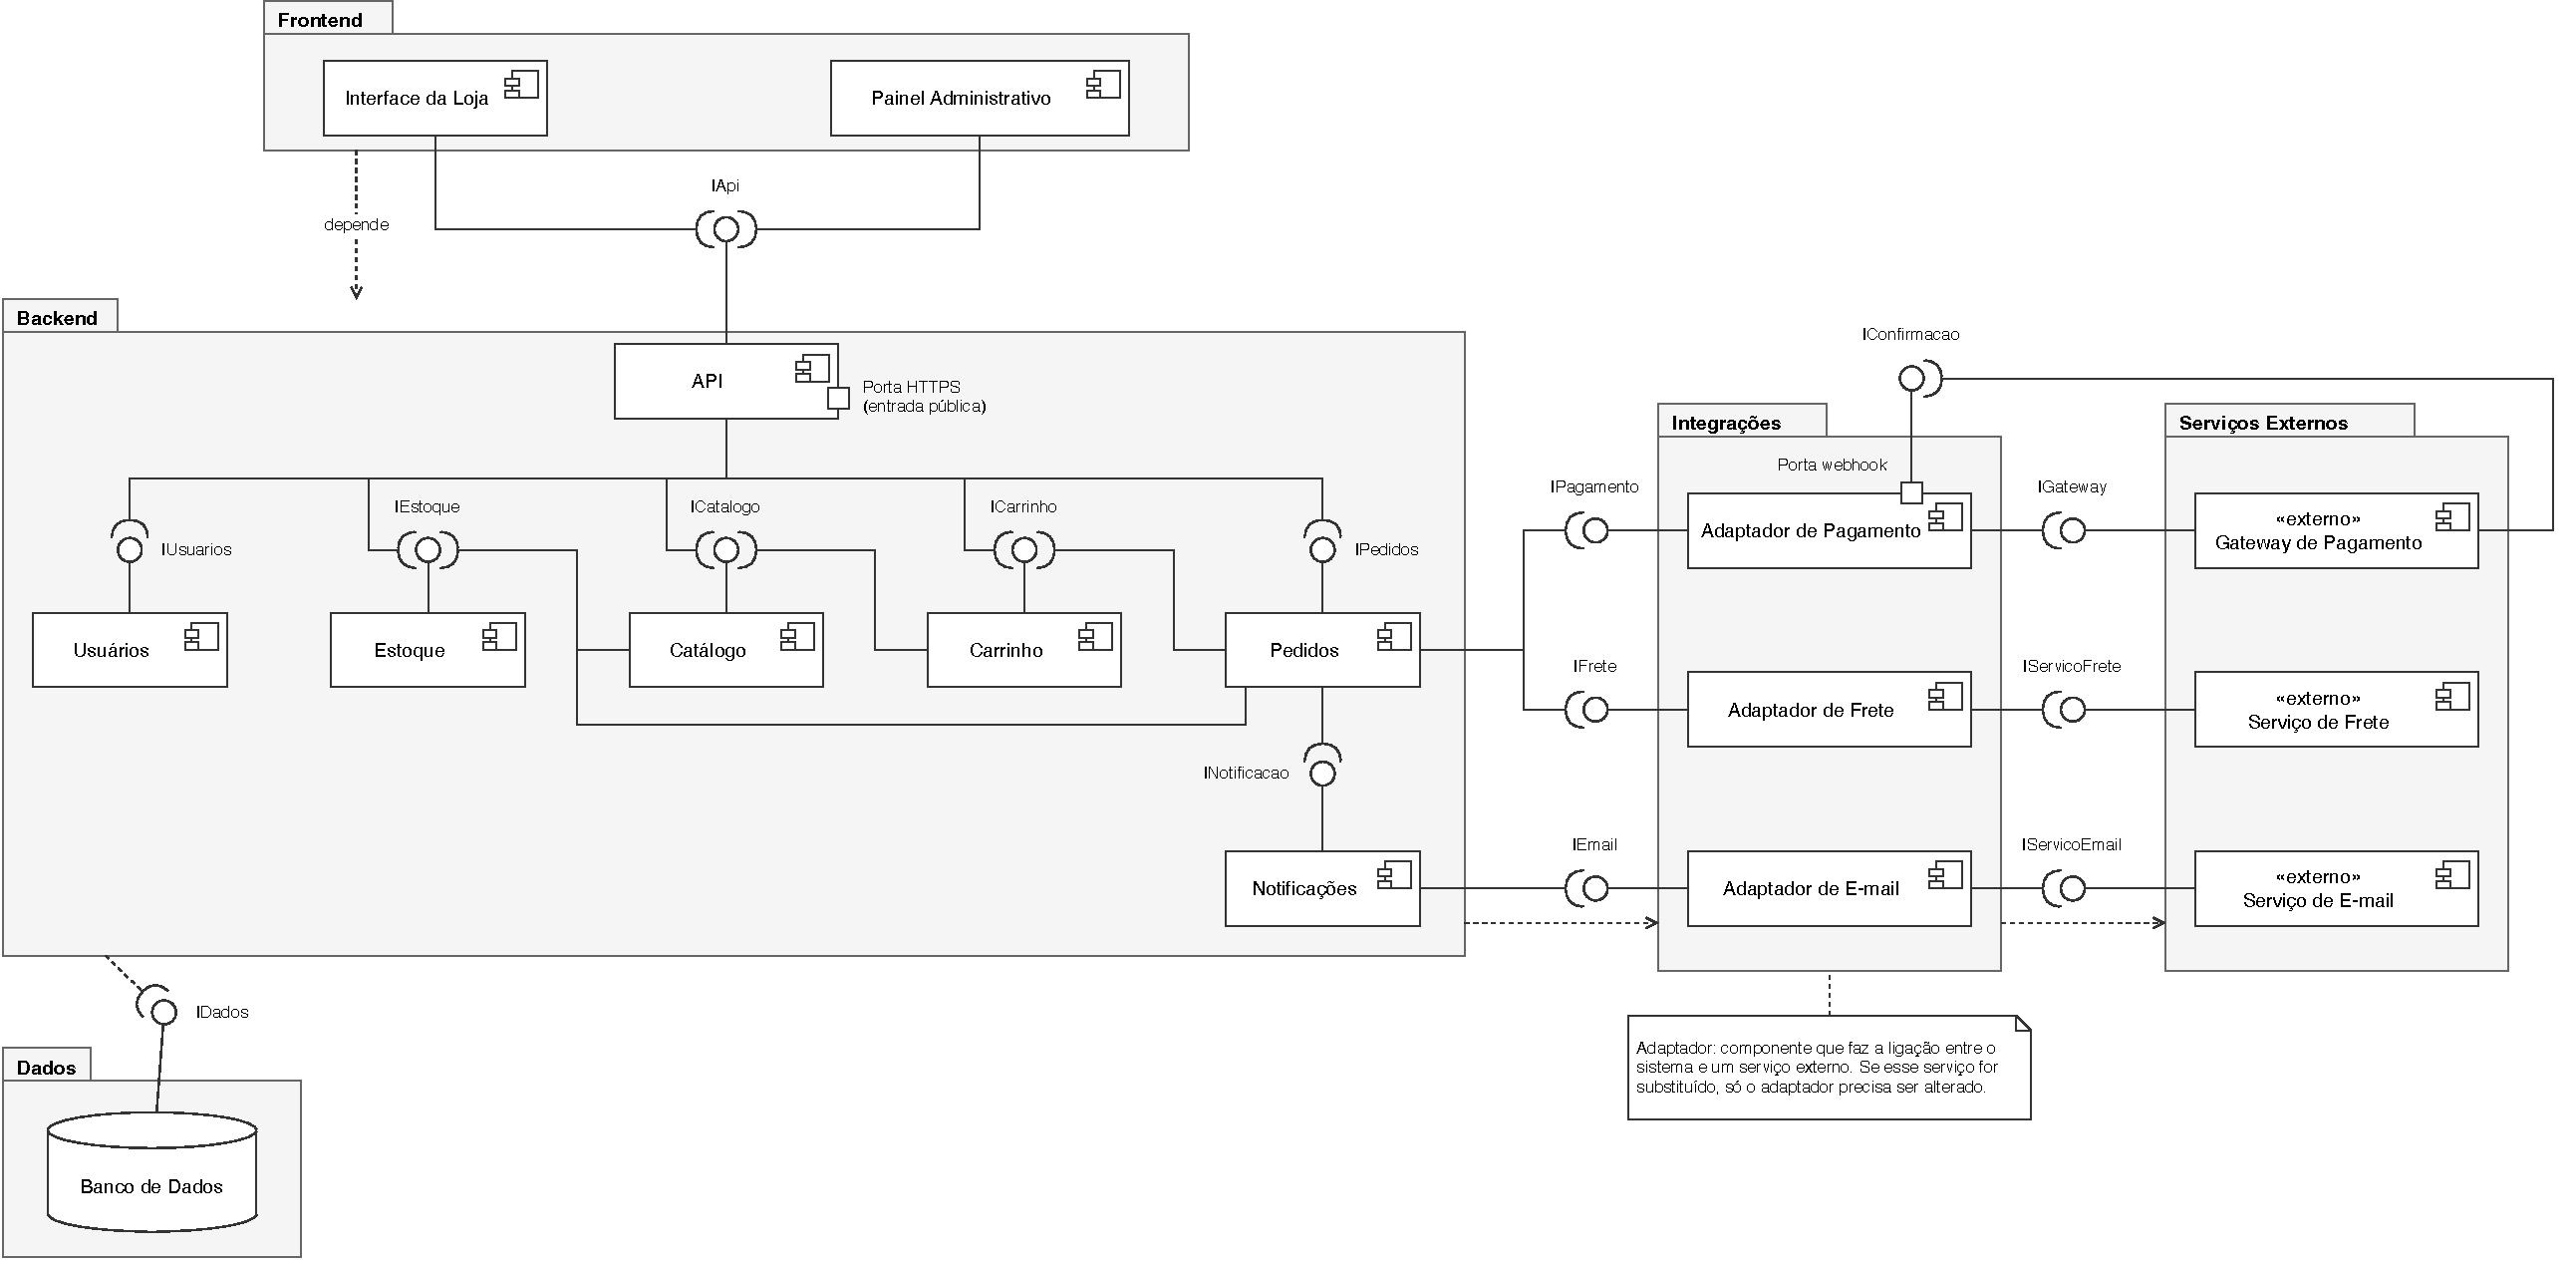
\includegraphics[trim=0.0bp 68.6bp 545.0bp 84.9bp, clip, width=265.0pt]{CMP_Geral.pdf}};
  \hl{132.4}{97.3}{177.2}{114.8}{PBack}
  \hl{244.5}{142.4}{283.9}{159.9}{Destaque}
  \pcard{298}{64.0}{131}{44.0}{PFront}{Frontend}{Telas da loja e do painel requerem \texttt{IApi}.}
  \pcard{298}{112.0}{131}{74.0}{PBack}{API e módulos}{A API fornece \texttt{IApi}; Usuários, Catálogo, Carrinho, Pedidos, Estoque e Notificações fornecem a sua.}
  \pcard{298}{190.0}{131}{47.0}{PDados}{Dados}{O Banco fornece \texttt{IDados}, usada pelos Repositórios.}
\end{tela}\end{frame}

% --- Luiz ---
\begin{frame}[plain]\begin{tela}
  \fundo{3.3}{DICIONÁRIO · INTEGRAÇÕES}{Adaptadores entre o sistema e os serviços externos}
    {Interfaces do lado do sistema e do lado do serviço (Tabelas 17 e 18)}
  \fill[white] \pto{25}{64} rectangle \pto{290}{237};
  \draw[Borda, line width=0.5pt] \pto{25}{64} rectangle \pto{290}{237};
  \node[anchor=north west, inner sep=0pt] at \pto{25.0}{64.0} {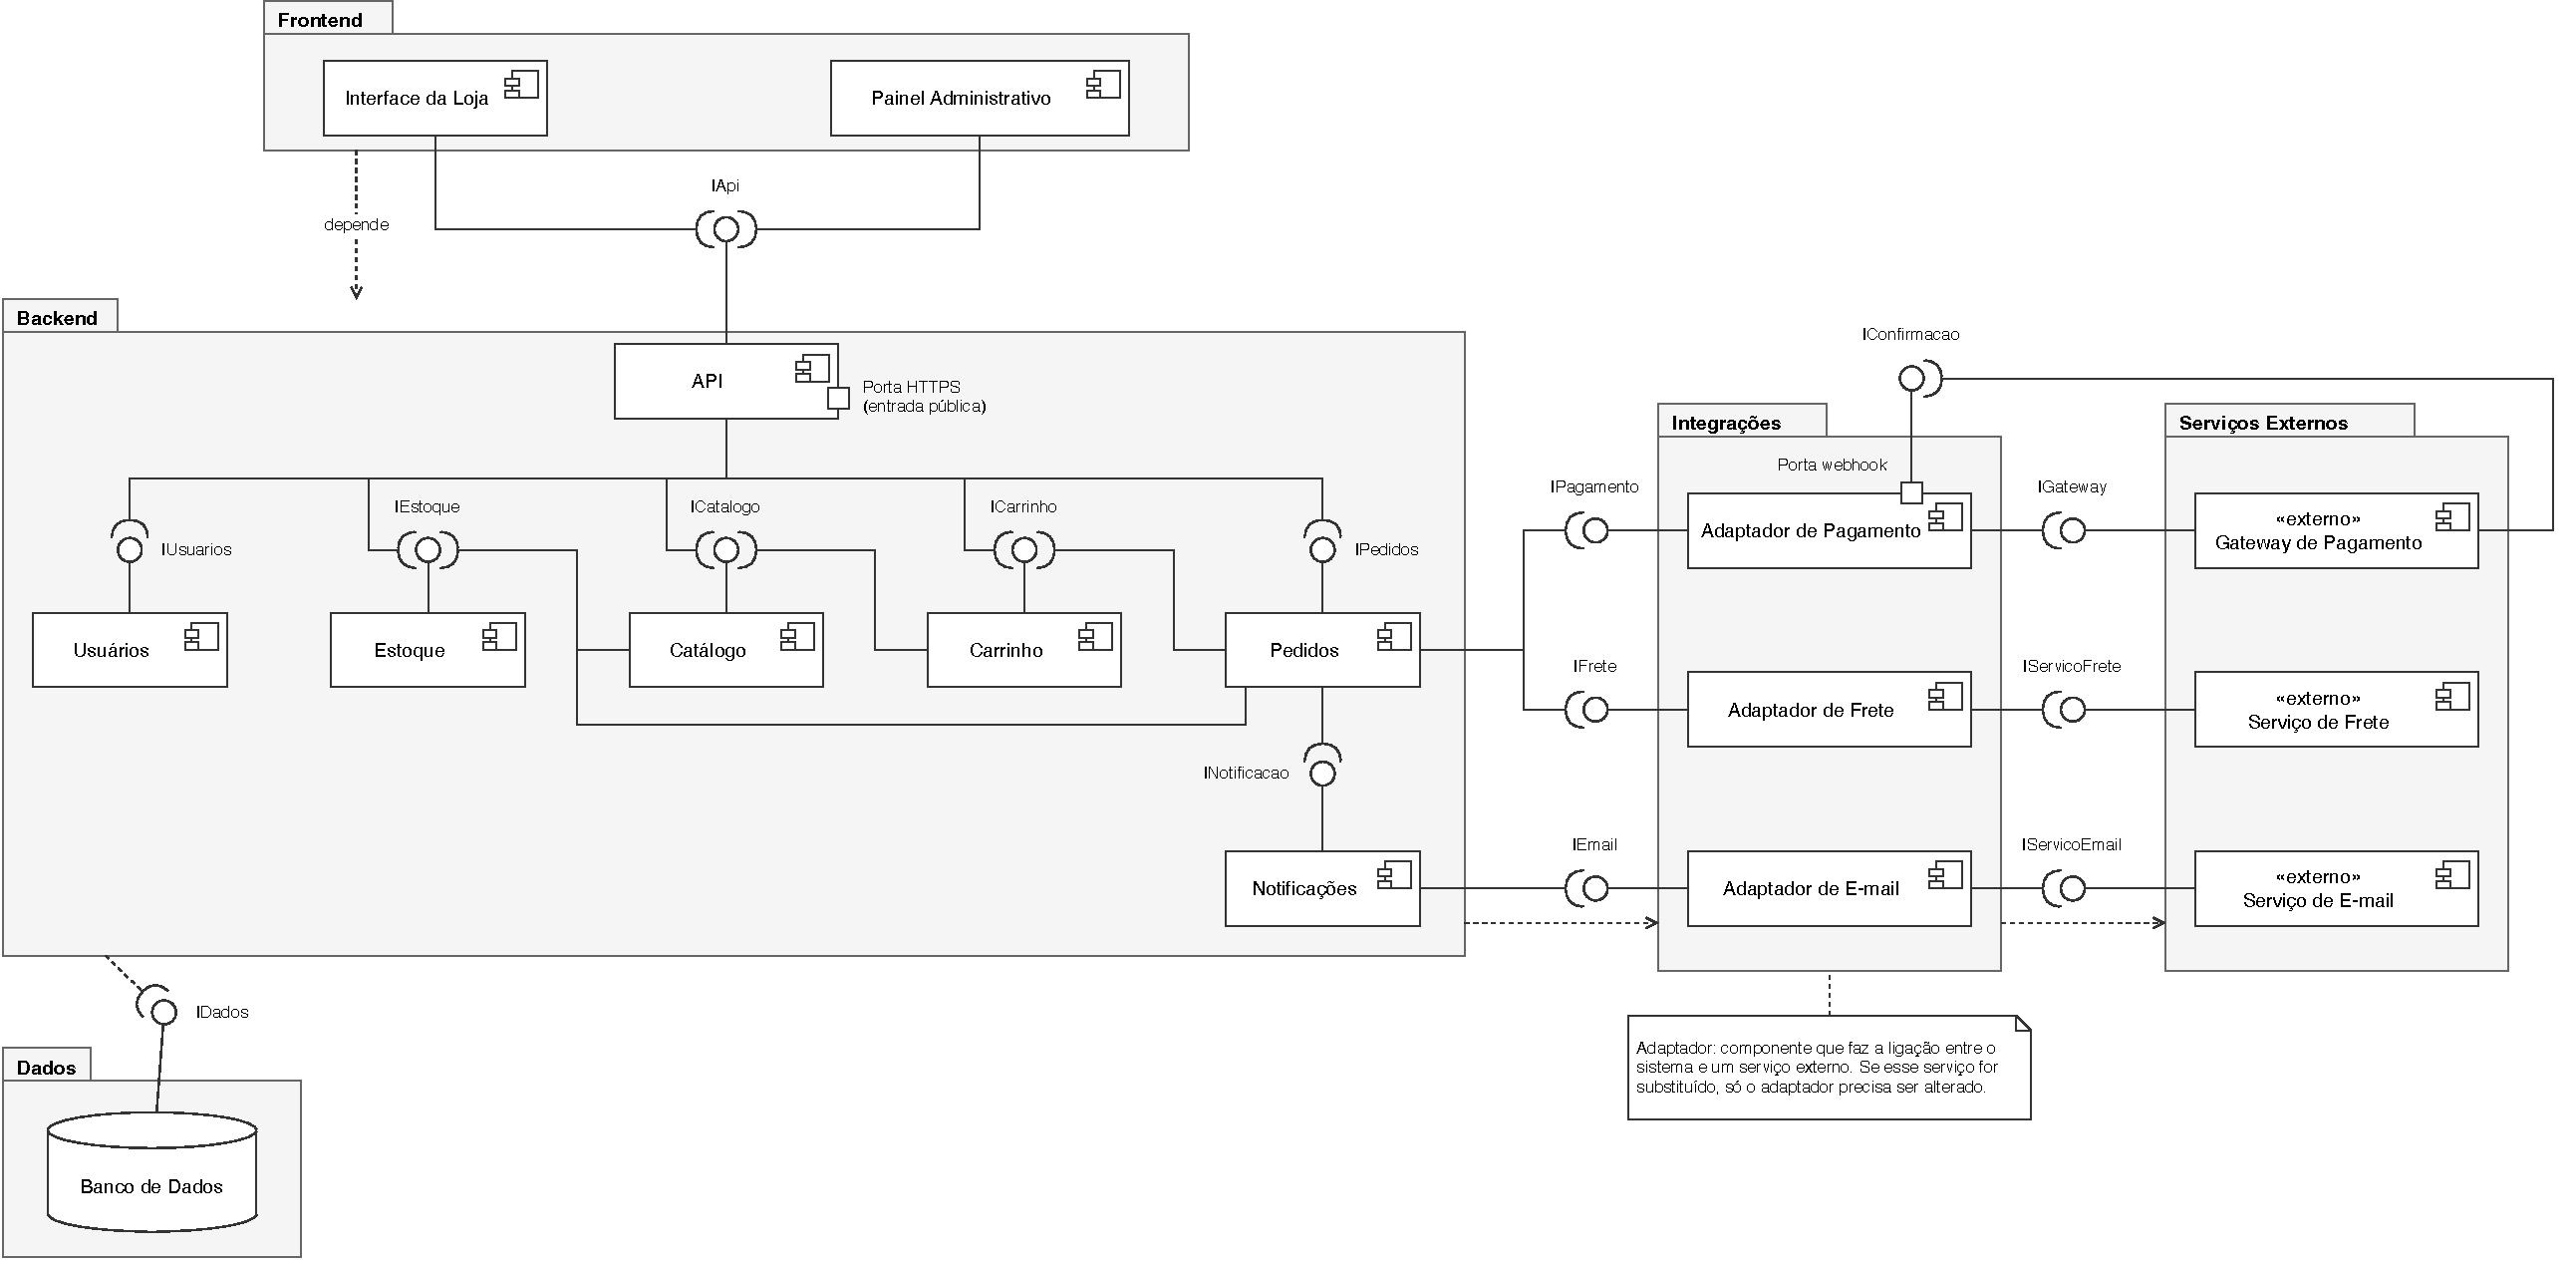
\includegraphics[trim=766.8bp 147.2bp 18.8bp 163.4bp, clip, width=265.0pt]{CMP_Geral.pdf}};
  \hl{43.8}{104.8}{129.1}{131.5}{Destaque}
  \pcard{298}{64.0}{131}{66.0}{PInt}{Adaptador de Pagamento}{Fornece \texttt{IPagamento} e \texttt{IConfirmacao}; requer \texttt{IGateway} e \texttt{IPedidos}.}
  \pcard{298}{134.0}{131}{41.0}{PInt}{Frete e E-mail}{Fornecem \texttt{IFrete} e \texttt{IEmail}.}
  \pcard{298}{179.0}{131}{58.0}{PExt}{Serviços Externos}{Terceiros: \texttt{IGateway}, \texttt{IServicoFrete}, \texttt{IServicoEmail}.}
\end{tela}\end{frame}

% --- Luiz ---
\begin{frame}[plain]\begin{tela}
  \fundo{3.3}{DEPENDÊNCIAS}{Por que cada dependência existe}
    {Cada seta tem um motivo registrado no documento (Tabela 19)}
  \fill[white] \pto{25}{64} rectangle \pto{290}{237};
  \draw[Borda, line width=0.5pt] \pto{25}{64} rectangle \pto{290}{237};
  \node[anchor=north west, inner sep=0pt] at \pto{25.0}{64.0} {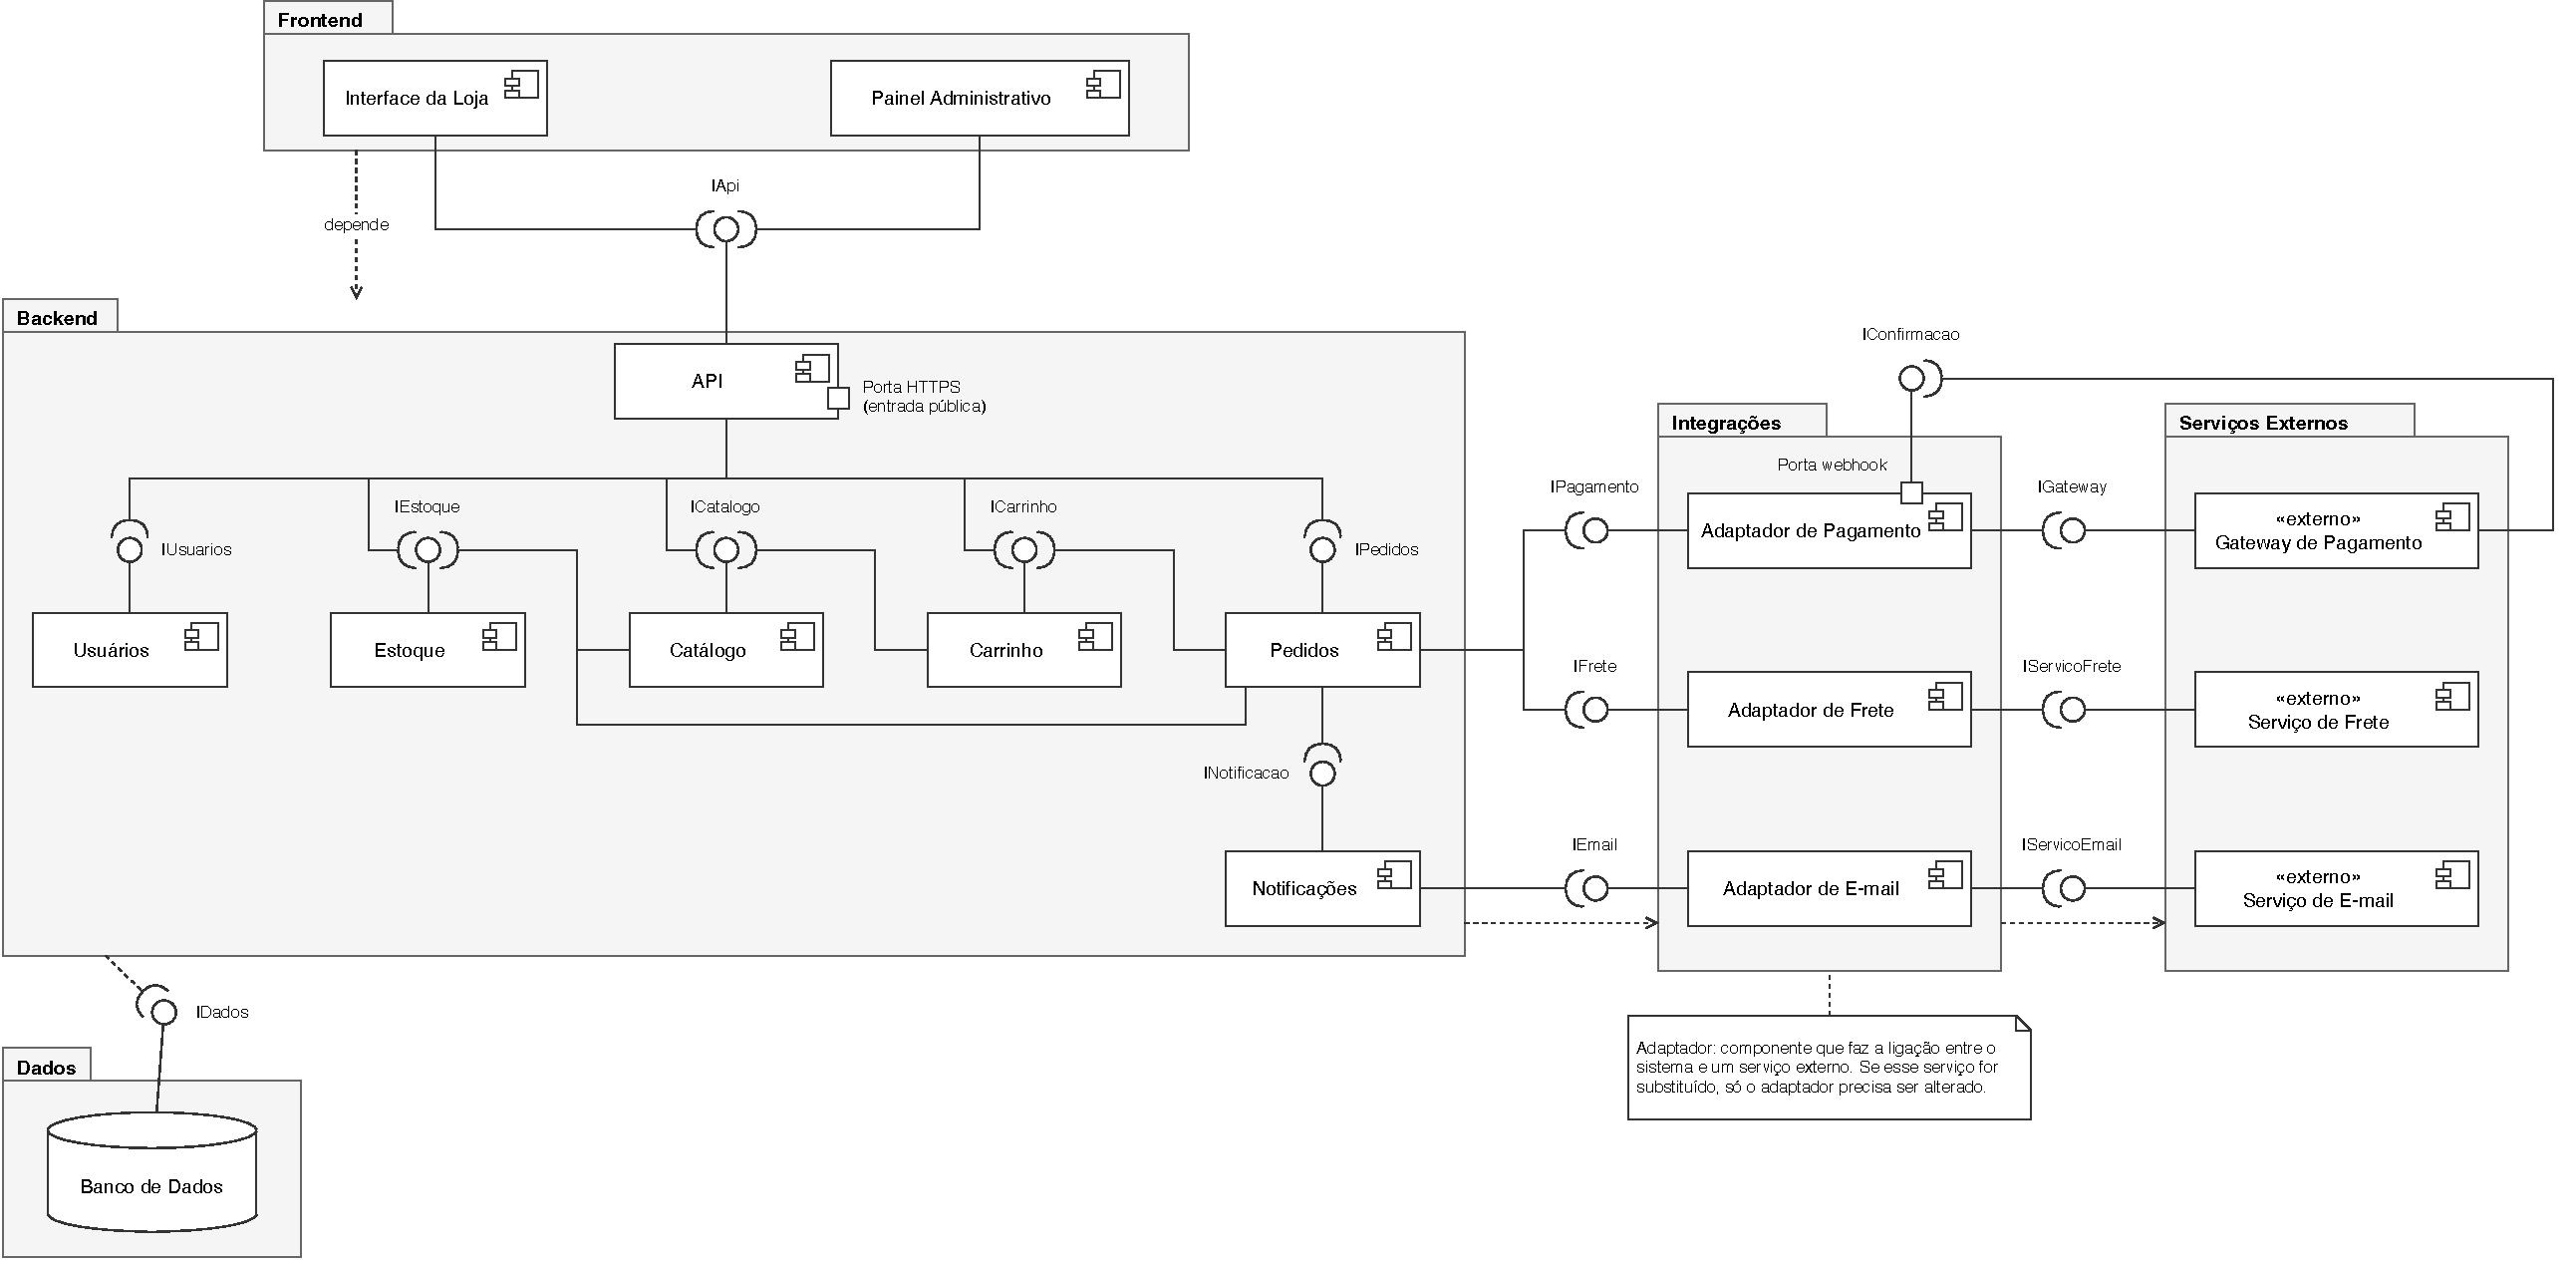
\includegraphics[trim=136.5bp 56.3bp 552.2bp 191.0bp, clip, width=265.0pt]{CMP_Geral.pdf}};
  \mk{98.7}{112.4}{1}
  \mk{167.6}{112.4}{2}
  \mk{236.6}{112.4}{3}
  \mk{236.6}{167.5}{4}
  \pnum{298}{64.0}{131}{40.2}{1}{Catálogo usa \texttt{IEstoque}: disponibilidade.}
  \pnum{298}{108.2}{131}{40.2}{2}{Carrinho usa \texttt{ICatalogo}: preço.}
  \pnum{298}{152.5}{131}{40.2}{3}{Pedidos usa carrinho, estoque, frete e pagamento.}
  \pnum{298}{196.8}{131}{40.2}{4}{Notificações usa \texttt{IEmail}: avisar.}
\end{tela}\end{frame}

% --- Yury ---
\begin{frame}[plain]\begin{tela}
  \fundo{3.4}{DETALHE INTERNO · FRONTEND}{Telas independentes e um único ponto de saída}
    {Cada tela atende casos de uso específicos (Figura 3 e Tabela 20)}
  \fill[white] \pto{25}{64} rectangle \pto{279.2937313432836}{237};
  \draw[Borda, line width=0.5pt] \pto{25}{64} rectangle \pto{279.2937313432836}{237};
  \node[anchor=north west, inner sep=0pt] at \pto{28.0}{64.0} {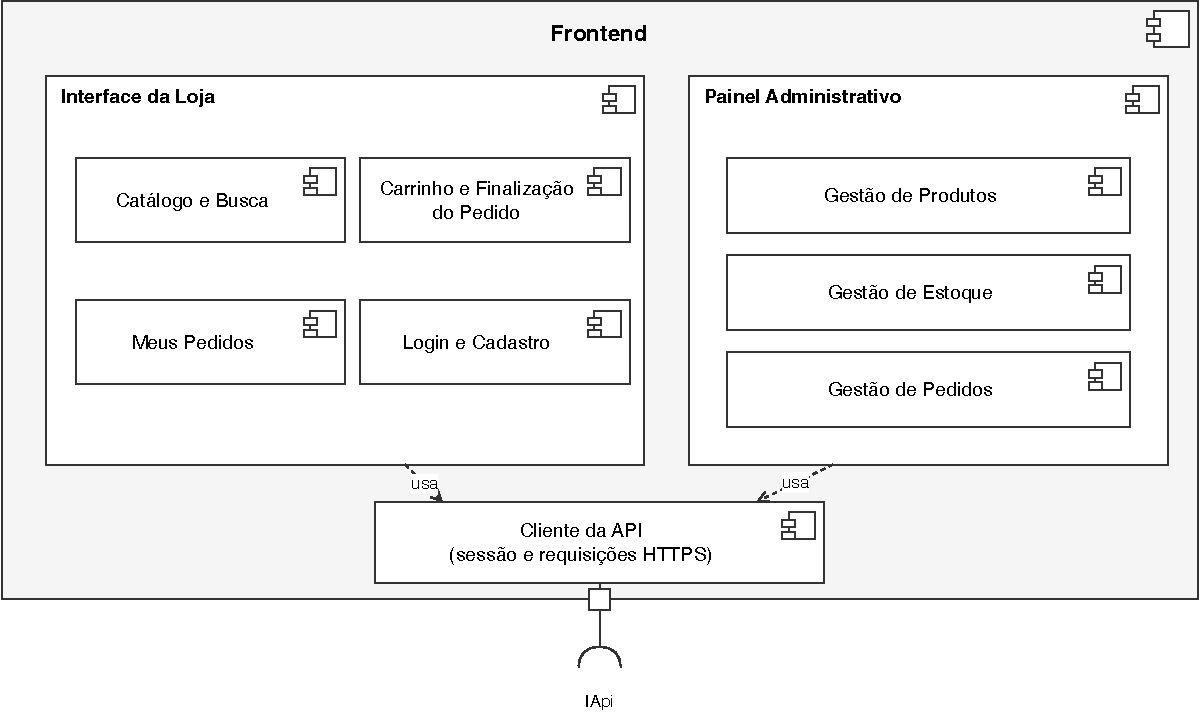
\includegraphics[trim=0.0bp 0.0bp 0.0bp 0.0bp, clip, width=248.3pt]{CMP_Frontend.pdf}};
  \hl{99.5}{183.0}{196.6}{204.0}{Destaque}
  \pcard{287.2937313432836}{64.0}{141.70626865671642}{74.0}{PFront}{Interface da Loja}{Catálogo e Busca (CU-01, 07), Carrinho e Finalização (CU-02, 03), Meus Pedidos (CU-04, 08), Login e Cadastro (CU-09, 12).}
  \pcard{287.2937313432836}{142.0}{141.70626865671642}{51.0}{PFront}{Painel Administrativo}{Login do Administrador (CU-09), Produtos e Estoque (CU-05), Pedidos (CU-06).}
  \pcard{287.2937313432836}{197.0}{141.70626865671642}{40.0}{Destaque}{Comunicação com a API}{Única que requer \texttt{IApi}; sessão e HTTPS.}
\end{tela}\end{frame}

% --- Yury ---
\begin{frame}[plain]\begin{tela}
  \fundo{3.5}{DETALHE INTERNO · BACKEND}{Três camadas e as mesmas portas do geral}
    {O componente API do geral se abre em controladores e segurança (Figura 4 e Tabela 21)}
  \fill[white] \pto{25}{64} rectangle \pto{269.97857421114134}{237};
  \draw[Borda, line width=0.5pt] \pto{25}{64} rectangle \pto{269.97857421114134}{237};
  \node[anchor=north west, inner sep=0pt] at \pto{28.0}{64.0} {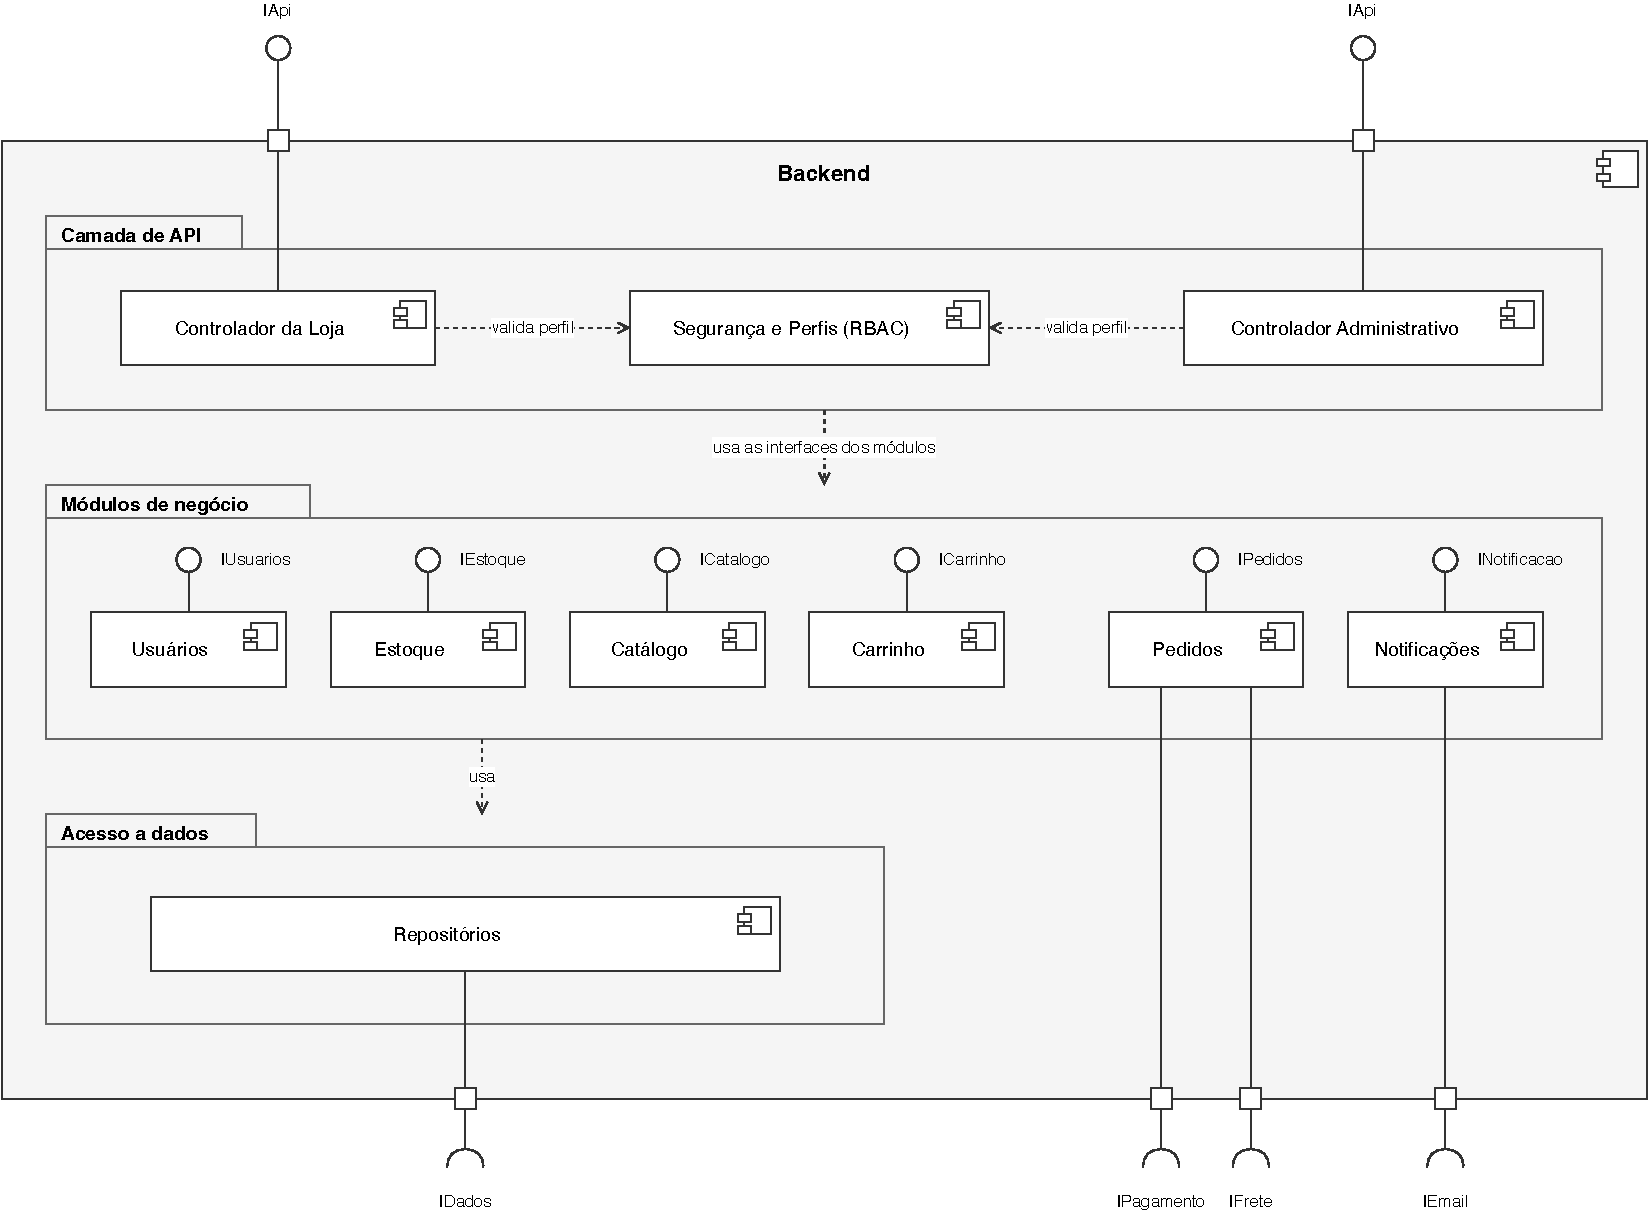
\includegraphics[trim=0.0bp 0.0bp 0.0bp 0.0bp, clip, width=239.0pt]{CMP_Backend.pdf}};
  \mk{32.0}{92.2}{1}
  \mk{32.0}{128.5}{2}
  \mk{32.0}{176.9}{3}
  \mk{63.0}{102.3}{4}
  \mk{88.2}{199.4}{5}
  \pnum{277.97857421114134}{64.0}{151.02142578885866}{31.4}{1}{\textbf{API:} controladores e Segurança e Perfis.}
  \pnum{277.97857421114134}{99.4}{151.02142578885866}{31.4}{2}{\textbf{Módulos:} usam as interfaces uns dos outros.}
  \pnum{277.97857421114134}{134.8}{151.02142578885866}{31.4}{3}{\textbf{Dados:} Repositórios requerem \texttt{IDados}.}
  \pnum{277.97857421114134}{170.2}{151.02142578885866}{31.4}{4}{\textbf{Topo:} duas portas \texttt{IApi}.}
  \pnum{277.97857421114134}{205.6}{151.02142578885866}{31.4}{5}{\textbf{Base:} saídas e a entrada \texttt{IPedidos}.}
\end{tela}\end{frame}

% =============================================================================
\section{Ferramenta e Apêndices}
% =============================================================================

% --- Yury ---
\begin{frame}[plain]\begin{tela}
  \fundo{4}{FERRAMENTA}{Ferramenta, símbolos e o que foi entregue}
    {Diagramas no draw.io, em notação UML 2.5 (Capítulo 4)}
  \cartao{25}{80}{128}{80}{Navy}{draw.io}{Os quatro diagramas foram feitos na ferramenta, com os símbolos da UML.}
  \cartao{163}{80}{128}{80}{Navy}{Lista de símbolos}{Tabelas 22 e 23: cada símbolo desenhado na própria ferramenta, com o significado.}
  \cartao{301}{80}{128}{80}{Navy}{Cores}{Só agrupam elementos; os diagramas continuam legíveis em preto e branco.}
  \faixa{170}{28}{Destaque}{Documento de projeto}
    {PDF com visão geral, 13 casos de uso especificados, diagrama geral, dois detalhes internos e dicionário de componentes.}
  \faixa{202}{26}{Navy}{Arquivos-fonte}
    {Os quatro diagramas em XML do draw.io, editáveis, junto do PDF no arquivo de entrega.}
\end{tela}\end{frame}

% --- Yury ---
\begin{frame}[plain]\begin{tela}
  \fundo{A · B}{APÊNDICES}{Dos requisitos aos componentes}
    {Os requisitos do Apêndice A dão origem aos casos de uso, que são atendidos pelos componentes}
  \tile{25}{80}{95}{72}{12}{Requisitos funcionais}{catálogo, carrinho, pedidos, admin}
  \tile{128}{80}{95}{72}{6}{Não funcionais}{HTTPS, perfil, responsivo}
  \tile{231}{80}{95}{72}{6}{Regras de negócio}{estoque, cancelamento, avisos}
  \tileD{334}{80}{95}{72}{B}{Glossário}{termos técnicos explicados}
  \node[anchor=north west, inner sep=0pt, text=Navy] at \pto{25}{162} {\fontsize{7.6pt}{9pt}\selectfont\bfseries Rastreabilidade de um requisito:};
  \chev{25}{176}{104}{40}{Claro}{Navy}{RF-06}{Finalizar pedido}
  \chev{125}{176}{104}{40}{Claro}{Navy}{CU-03}{Finalizar Pedido}
  \chev{225}{176}{104}{40}{PFront}{white}{Carrinho e Finalização}{tela do Frontend}
  \chev{325}{176}{104}{40}{PBack}{white}{Pedidos}{módulo do Backend}
\end{tela}\end{frame}

% --- Yury ---
\begin{frame}[plain]\begin{tela}
  \fundo{CONCLUSÃO}{COMO OS MODELOS SE CONECTAM}{Dois diagramas que contam a mesma história}
    {O que o sistema faz, para quem, e como as partes conversam}
  \painel{25}{80}{160}{148}{SÍNTESE}{Cada caso de uso tem onde acontecer na arquitetura}
    {Os atores secundários do diagrama de casos de uso viram adaptadores; cada dependência entre componentes tem um motivo registrado.}
  \cartao{195}{80}{234}{46}{Principal}{Casos de uso}{O que o sistema faz e para quem, com as regras de cada fluxo nas 13 tabelas.}
  \cartao{195}{131}{234}{46}{PBack}{Componentes: geral}{Como o sistema é dividido em pacotes e como as partes se ligam por interfaces.}
  \cartao{195}{182}{234}{46}{PFront}{Componentes: detalhes}{O interior do Frontend e do Backend, com as mesmas interfaces na borda.}
\end{tela}\end{frame}

% =============================================================================
\setLayout{blank}
\setBGColor{UFGBlue}
\begin{frame}[plain,noframenumbering]{}
    \fonteTela
    \centering
    \vspace{0.6cm}
    {\Huge \textbf{Obrigado!}}\par\vspace{0.4cm}
    {\Large Site de Loja de Eletrônicos (E-commerce)}\par\vspace{0.2cm}
    {\normalsize Modelagem de Software -- APS2 | UFG / INF (2026/2)}\par\vspace{1.5cm}
    {\large \textbf{Dúvidas e Discussão}}\par\vspace{0.5cm}
    
\includegraphics[width=0.42\textwidth]{lib/logos/ES-INF-full-white.png}
\end{frame}

\end{document}
